%%%%%%%%%%%%%%%%%%%%%%%%%%%%%%%%%%%%%%%%%%%%%%%%%%%%%%%%%%%%%%%%%%%%%%
% Lớp 11 | Hàm số mũ và hàm số lôgarít | Phương trình, bất phương trình mũ và lôgarít
% Dạng 1D6?4-5: Bất phương trình mũ, lôgarít đưa về cùng cơ số
% Số câu: 127  (sinh tự động bởi tach_cau.py; từ nay thầy sửa trực tiếp file này)
%%%%%%%%%%%%%%%%%%%%%%%%%%%%%%%%%%%%%%%%%%%%%%%%%%%%%%%%%%%%%%%%%%%%%%

%%%%%%%%%%%%%%%% TRẮC NGHIỆM 4 PHƯƠNG ÁN %%%%%%%%%%%%%%%%

% nguồn: Ok_Toan11_TracNghiem_Lan2
\begin{ex}%[1D6N4-5]%[ma:7f74f579]
	Tập nghiệm của phương trình ${5^{x-2}}\le \dfrac{1}{5}$  là
	 \choice
		 {$\left[1;+\infty \right)$}
		 {$\left(-\infty;0\right)$}
		{$\left[2;+\infty  \right)$}
		{\True $\left(-\infty;1\right]$} 
	 \loigiai{
		Ta  có ${5^{x-2}}\le \dfrac{1}{5}\Leftrightarrow x-2\le-1\Leftrightarrow x\le 1$.\\
		Tập  nghiệm của phương trình là $\left(-\infty;1\right]$.\\
	 }
\end{ex}

% nguồn: Ok_Toan11_TracNghiem_Lan2
\begin{ex}%[1D6N4-5]%[ma:e8aaa4aa]
	Tập nghiệm của  bất phương trình $3^x<2$ là
	\choice 
		{\True  $\left(-\infty;{{\log}_3}2\right)$}
		{$\left(-\infty;{{\log}_2}3\right)$} 
		{$\left({{\log}_3}2;+\infty \right)$} 
		{$\left({{\log}_2}3;+\infty  \right)$}
	\loigiai{Ta có $3^x<2\Leftrightarrow  x<{{\log}_3}2$.\\
	Do đó tập nghiệm $S=\left(-\infty;{{\log}_3}2\right)$.} 
\end{ex}

% nguồn: Ok_Toan11_TracNghiem_Lan2
\begin{ex}%[1D6N4-5]%[ma:6a5fb478]
	Tập  nghiệm của bất phương trình $\left(\dfrac{3}{4}\right)^{x-1}>\left(\dfrac{3}{4}\right)^{-x+3}$ là
	\choice 
		{ $\left(2;+\infty\right)$} 
		{\True$\left(-\infty;2\right)$} 
		{$\left[2;+\infty\right)$} 
		 {$\left(-\infty;2\right]$}
	 \loigiai{Vì $\dfrac{3}{4}<1$ nên $\left(\dfrac{3}{4}\right)^{x-1}>\left(\dfrac{3}{4}\right)^{-x+3} \Leftrightarrow x-1<-x+3 \Leftrightarrow 2x<4 \Leftrightarrow x<2$. \\
	Vậy tập nghiệm của bất phương trình  là $\left(-\infty;2\right)$.}
\end{ex}

% nguồn: Ok_Toan11_TracNghiem_Lan2
\begin{ex}%[1D6N4-5]%[ma:dc325df4]
	Tập các nghiệm của bất  phương trình $2^x>6$ là
	\choice 
		{\True $\left({{\log}_2}6;+\infty  \right)$}
		 {$\left(-\infty;3\right)$}
		{$\left(3;+\infty \right)$} 
		 {$\left(-\infty;{{\log}_2}6\right)$}
	 \loigiai{$2^x>6\Leftrightarrow x>{{\log}_2}6\Leftrightarrow x\in \left({{\log}_2}6;+\infty \right)$.}
\end{ex}

% nguồn: Ok_Toan11_TracNghiem_Lan2
\begin{ex}%[1D6N4-5]%[ma:5b3e68a9]
	Tập nghiệm của  phương trình: ${2^{x+1}}{{.3}^x}\le 72$ là
	 \choice
		{$\left(2;+\infty \right)$} 
		{$\left(-\infty;2\right)$} 
		{\True  $\left(-\infty;2\right]$}
		{$\left[2;+\infty \right)$} 
	\loigiai{Ta có: ${2^{x+1}}{{.3}^x}\le 72\Leftrightarrow {2^x}{{.3}^x}.2\le 72\Leftrightarrow {6^x}\le  36\Leftrightarrow x\le 2$.\\
		Vậy  tập nghiệm của bất phương trình là $\left(-\infty;2\right]$.
	} 
\end{ex}

% nguồn: Ok_Toan11_TracNghiem_Lan2
\begin{ex}%[1D6N4-5]%[ma:a5b6749d]
	Tập nghiệm của bất phương  trình $4^x\ge 2$ là
	\choice 
		{$\left(\dfrac{1}{4};+\infty  \right)$}
		{$\left[\dfrac{1}{4};+\infty \right)$} 
		{\True $\left[\dfrac{1}{2};+\infty  \right)$}
		 {$\left(\dfrac{1}{2};+\infty \right)$}
	 \loigiai{Ta có:\\
		$4^x\ge 2\Leftrightarrow  {2^{2x}}\ge {2^1}\Leftrightarrow 2x\ge 1\Leftrightarrow x\ge \dfrac{1}{2}$.\\
	 Vậy $S=\left[\dfrac{1}{2};+\infty \right)$.}
\end{ex}

% nguồn: Ok_Toan11_TracNghiem_Lan2
\begin{ex}%[1D6N4-5]%[ma:28014913]
	Tập nghiệm của bất  phương trình ${5^{2x+3}}>\dfrac{1}{25}$ là
	 \choice
		 {\True $\left(-\dfrac{5}{2};+\infty \right)$}
		{$\left(-\infty;-\dfrac{5}{2}  \right)$}
		{$\left(0;+\infty  \right)$}
		{$\left(-\dfrac{1}{2};+\infty  \right)$}
	\loigiai{Ta  có: ${5^{2x+3}}>\dfrac{1}{25}\Leftrightarrow {5^{2x+3}}>{5^{-2}}\Leftrightarrow 2x+3>-2\Leftrightarrow x>-\dfrac{5}{2}$.\\
	Vậy tập nghiệm của bất phương trình đã  cho là$S=\left(-\dfrac{5}{2};+\infty \right)$.}
\end{ex}

% nguồn: Ok_Toan11_TracNghiem_Lan2
\begin{ex}%[1D6N4-5]%[ma:34d9b29d]
	Tập  nghiệm của bất phương trình $\left(\dfrac{1}{2}\right)^{x^2-x}>2^{x-4}$ là
	 \choice
		{  $\left(-2;+\infty\right)$}
		 {$\left(-\infty;-2\right) \cup \left(2;+\infty\right)$}
		 {$\left(2;+\infty\right)$}
		{\True  $\left(-2;2\right)$}
	\loigiai{$\left(\dfrac{1}{2}\right)^{x^2-x}>2^{x-4} \Leftrightarrow 2^{-(x^2-x)} >2^{x-4} \Leftrightarrow -x^2+x>x-4 \Leftrightarrow -x^2+4>0  \Leftrightarrow -2<x<2$.\\
	Vậy  tập nghiệm của bất phương trình là $\left(-2;2\right)$.}
\end{ex}

% nguồn: Ok_Toan11_TracNghiem_Lan2
\begin{ex}%[1D6N4-5]%[ma:ef99a3e1]
	Nghiệm của phương trình $3^x<5$  là
	 \choice
		 {$x>{{\log}_3}5$}
		 {$x>{{\log}_3}3$}
		 {\True $x<{{\log}_3}5$}
		 {$x<{{\log}_3}3$}
	\loigiai{Ta có $3^x<5\Leftrightarrow  x<{{\log}_3}5$.}
\end{ex}

% nguồn: Ok_Toan11_TracNghiem_Lan2
\begin{ex}%[1D6N4-5]%[ma:9ad24d13]
	Tập nghiệm của bất phương trình ${2^{2x}}<{2^{x+4}}$ là 
	\choice 
		{\True  $\left(-\infty;4\right)$}
		{$\left(0;4\right)$} 
		{$\left(0;16\right)$} 
		{$\left(4;+\infty \right)$} 
	\loigiai{Ta có  ${2^{2x}}<{2^{x+4}}\Leftrightarrow 2x<x+4\Leftrightarrow x<4$.\\
	Tập nghiệm của bất phương trình $S=\left(-\infty;4\right)$.} 
\end{ex}

% nguồn: Ok_Toan11_TracNghiem_Lan2
\begin{ex}%[1D6N4-5]%[ma:5f133b1c]
	Tập nghiệm  của bất phương trình $2^x\le 4$ là
	 \choice
		{\True $\left(-\infty;2\right]$} 
		 {$\left[0;2\right]$}
		{$\left(-\infty;2\right)$} 
		 {$\left(0;2\right)$}
	\loigiai{Ta có $2^x\le  4\Leftrightarrow x\le 2$.\\
	Tập nghiệm của  bất phương trình là $\left(-\infty;2\right]$.}
\end{ex}

% nguồn: Ok_Toan11_TracNghiem_Lan2
\begin{ex}%[1D6N4-5]%[ma:f273348b]
	Tập  nghiệm của bất phương trình $3^x>9$ là
	\choice 
		{\True $\left(2;+\infty \right)$} 
		{$\left(0;2\right)$} 
		{$\left(0;+\infty  \right)$}
		 {$\left(-2;+\infty \right)$}
	 \loigiai{Ta có $3^x>9\Leftrightarrow {3^x}>3^2\Leftrightarrow x>2\Leftrightarrow x\in \left(2;+\infty \right)$.\\
	Tập nghiệm của bất  phương trình $3^x>9$ là $\left(2;+\infty \right)$.}
\end{ex}

% nguồn: Ok_TracNghiemLop11_Lan1
\begin{ex}%[1D6N4-5]%[ma:ff54f09d]
	 Tập nghiệm $S$ của bất phương trình $\log_2(x-1)>0$ là
	 \choice
		{\True $S=\left(2;+\infty\right)$} 
		{$S=\left(1;+\infty\right)$} 
		 {$S=\varnothing$}
		 {$S=\mathbb{R}$}
	\loigiai{ 
		Ta có $\log_2(x-1)>0\Rightarrow x-1>1\Rightarrow  x>2$.
	 }
\end{ex}

% nguồn: Ok_TracNghiemLop11_Lan1
\begin{ex}%[1D6N4-5]%[ma:215d6478]
	Tập nghiệm của bất  phương trình $2^x < 5$ là
	 \choice
		{\True $\left(-\infty;\log_2  5\right)$}
		 {$\left(\log_25;+\infty\right)$}
		{$\left(-\infty;\log_5  2\right)$}
		{$\left(\log_52;+\infty\right)$} 
	 \loigiai{
		Ta có $2^x <  5\Leftrightarrow x<\log_2 5$.\\
		Tập nghiệm của bất phương trình $2^x <  5$ là $S=\left(-\infty;\log_2 5\right)$.
	 }
\end{ex}

% nguồn: Ok_Toan11_TracNghiem_Lan2
\begin{ex}%[1D6H4-5]%[ma:f647329a]
	Tập nghiệm $  S$ của bất phương trình $\log_2\left(11-5x\right)-3\log_8\left(x-1\right)\ge 0$ là
	\choice 
		{$ S=\left(1;\dfrac{5}{3}\right]$} 
		{\True  $ S=\left(1;2\right]$}
		{$  S=\left[2;\dfrac{11}{5}\right)$}
		{$ S=\left[\dfrac{5}{3};\dfrac{11}{5}\right)$} 
	 \loigiai{
		Điều kiện  $\heva{&11-5x>0\\&x-1>0}\Leftrightarrow\heva{&x<\dfrac{11}{5}\\&x>1}\Leftrightarrow 1<x<\dfrac{11}{5}$.\\
		 Bất phương trình tương đương
		 \allowdisplaybreaks
		\begin{eqnarray*}
			 \log_2\left(11-5x\right)-3\log_8\left(x-1\right)\ge 0&\Leftrightarrow&{\log_2}\left(11-5x\right)-3\log_{2^3}\left(x-1\right)\ge 0\\
			 &\Leftrightarrow&{\log_2}\left(11-5x\right)-\log_2\left(x-1\right)\ge 0\\
			&\Leftrightarrow&{\log_2}\left(11-5x\right)\ge{\log_2}\left(x-1\right)\\ 
			&\Leftrightarrow&11-5x\ge  x-1\\
			&\Leftrightarrow&x\le2. 
		\end{eqnarray*}
		Kết hợp điều  kiện $\Rightarrow 1 < x\le 2$.\\
		 Vậy tập nghiệm của bất phương trình là $ S=\left(1;2\right]$.
	 }
\end{ex}

% nguồn: Ok_Toan11_TracNghiem_Lan2
\begin{ex}%[1D6H4-5]%[ma:b89af054]
	Tập nghiệm $S$ của bất phương  trình $5^{x+2}\ge \left(\dfrac{1}{25}\right)^{-x}$ là
	 \choice
		{  $S=\left(1;+\infty\right)$}
		 {\True $\left(-\infty;2\right]$}
		{$\left[2;+\infty\right)$} 
		{$\left(-\infty;2\right)$} 
	\loigiai{\allowdisplaybreaks 
	\begin{align*}
		5^{x+2}\ge \left(\dfrac{1}{25}\right)^{-x} &\Leftrightarrow  5^{x+2}\ge \left(5^{-2}\right)^{-x}\\
		&\Leftrightarrow 5^{x+2}\ge  5^{2x}\\
		&\Leftrightarrow x+2 \ge 2x  \\
		&\Leftrightarrow  -x \ge -2\\
		&\Leftrightarrow x  \le 2.
	\end{align*}
	Vậy tập nghiệm của  bất phương trình là $\left(-\infty;2\right]$.}
\end{ex}

% nguồn: Ok_Toan11_TracNghiem_Lan2
\begin{ex}%[1D6H4-5]%[ma:9f362843]
	Bất phương trình $\log_2\left(3x-2\right) >\log_2\left(6-5x\right)$ có tập  nghiệm là
	 \choice
		 {$\left(\dfrac{1}{2};\,3\right)$}
		 {$\left(-\,3;\,1\right)$}
		{$\left(0;\,+\infty\right)$} 
		{\True $\left(1;\,\dfrac{6}{5}\right)$} 
	 \loigiai{
		Ta  có $\log_2\left(3x-2\right) >\log_2\left(6-5x\right)\Leftrightarrow \heva{&3x-2 > 0\\&
		6-5x >  0\\
		&3x-2  > 6-5x}\Leftrightarrow \heva{&x >\dfrac{2}{3}\\
		 &x <\dfrac{6}{5}\\
		&x > 1}\Leftrightarrow 1  < x <\dfrac{6}{5}.$\\
	Vậy tập  nghiệm của bất phương trình là $ S=\left(1;\dfrac{6}{5}\right).$}
\end{ex}

% nguồn: Ok_Toan11_TracNghiem_Lan2
\begin{ex}%[1D6H4-5]%[ma:5efa8ffd]
	Tìm tập nghiệm $S$ của bất phương trình $\log_{\frac{1}{3}}\left(1-x\right) >\log_{\frac{1}{3}}\left(2x+3\right)$. 
	\choice 
		 {$ S=\left(-\infty;-\dfrac{2}{3}\right)$}
		{$  S=\left(-\dfrac{2}{3};+\infty\right)$}
		 {\True $ S=\left(-\dfrac{2}{3};1\right)$}
		{$ S=\left(1;+\infty\right)$} 
	 \loigiai{
		Bất phương trình tương đương với $\left\{\begin{array}{l}
		1-x >  0\\
		1-x  < 2x+3
	\end{array}\right.$$\Leftrightarrow\left\{\begin{array}{l}
	 x < 1\\
	 x >-\dfrac{2}{3}
	\end{array}\right.$$\Leftrightarrow-\dfrac{2}{3}< x < 1$.\\
	Vậy  tập nghiệm của bất phương trình là
	$S=\left(-\dfrac{2}{3};1\right)$. 
	} 
\end{ex}

% nguồn: Ok_Toan11_TracNghiem_Lan2
\begin{ex}%[1D6H4-5]%[ma:88930c10]
	Bất phương trình  $\left(\dfrac{2}{3}\right)^{x^2-3x}<\left(\dfrac{9}{4}\right)^{x-1}$ tương đương với bất phương trình nào sau đây?
	\choice 
		 {$x^2-5x-2<0$}
		 {$x^2-5x+2<0$}
		{\True  $-x^2+x+2<0$}
		 {$-x^2-x-2<0$}
	 \loigiai{\allowdisplaybreaks
		\begin{align*}
			 \left(\dfrac{2}{3}\right)^{x^2-3x}<\left(\dfrac{9}{4}\right)^{x-1} &\Leftrightarrow \left(\dfrac{2}{3}\right)^{x^2-3x}<\left( \left(\dfrac{2}{3}\right)^{-2}\right)^{x-1}\\
			 &\Leftrightarrow \left(\dfrac{2}{3}\right)^{x^2-3x}<\left(\dfrac{2}{3}\right)^{-2(x-1)}\\
			&\Leftrightarrow x^2-3x >  -2(x-1)\\
			&\Leftrightarrow x^2-3x>-2x+2\\ 
			&\Leftrightarrow x^2-x-2>0\\ 
			&\Leftrightarrow  -x^2+x+2<0.
	\end{align*}}
\end{ex}

% nguồn: Ok_Toan11_TracNghiem_Lan2
\begin{ex}%[1D6H4-5]%[ma:27a274c0]
	Tập  nghiệm của bất phương trình $\log_2\left(2x^2-x\right)\le{\log_{\sqrt 2}}x$ là
	 \choice
		{$\left[\dfrac{1}{2};1\right]$} 
		{$ (0;1)$} 
		 {$\left[0;1\right]$}
		{\True  $\left(\dfrac{1}{2};1\right]$}
	 \loigiai{
		Điều kiện $\heva{&2x^2-x > 0\\&x > 0}\Leftrightarrow x>\dfrac{1}{2}$.\\ 
		$\log_2\left(2x^2-x\right)\le{\log_{\sqrt 2}}x$ $\Leftrightarrow{\log_2}\left(2x^2-x\right)\le{\log_2}{x^2}$ $\Leftrightarrow 2x^2-x\le{x^2}\Leftrightarrow{x^2}-x\le 0\Leftrightarrow 0 < x\le 1$.\\ 
		Vậy tập nghiệm của bất phương trình là  $\left(\dfrac{1}{2};1\right]$.
	 }
\end{ex}

% nguồn: Ok_Toan11_TracNghiem_Lan2
\begin{ex}%[1D6H4-5]%[ma:f8f00898]
	Tập nghiệm của bất  phương trình $\log_{\frac{1}{2}}\left(3x-2\right) >\log_{\frac{1}{2}}\left(4-x\right)$ là
	 \choice
		 {$ S=\left(\dfrac{2}{3};3\right)$}
		{$ S=\left(-\infty;\dfrac{3}{2}\right)$} 
		 {\True $ S=\left(\dfrac{2}{3};\dfrac{3}{2}\right)$}
		 {$ S=\left(\dfrac{3}{2};4\right)$}
	\loigiai{ 
		Điều kiện $\heva{&3x-2>0\\&4-x>0}\Leftrightarrow  \heva{&x>\dfrac{2}{3}\\&x<4}\Leftrightarrow \dfrac{2}{3}<x<4$.\\
		Trong điều kiện  trên, ta có
		$$\log_{\frac{1}{2}}\left(3x-2\right) >\log_{\frac{1}{2}}\left(4-x\right)\Leftrightarrow  3x-2 < 4-x\Leftrightarrow x <\dfrac{3}{2}.$$
		So với  điều kiện ta được $\dfrac{2}{3}< x <\dfrac{3}{2}$.\\
		Vậy  tập nghiệm của bất phương trình $ S=\left(\dfrac{2}{3};\dfrac{3}{2}\right)$.
	} 
\end{ex}

% nguồn: Ok_Toan11_TracNghiem_Lan2
\begin{ex}%[1D6H4-5]%[ma:2111cd4e]
	Bất phương trình $\log_2\left(\log_{\frac{1}{3}}\dfrac{3x-7}{x+3}\right)\ge 0$ có tập nghiệm  là $\left(a;b\right]$. Tính giá trị $P=3a-b$.
	\choice 
		 {\True $P=4\cdot $}
		{$P=5\cdot $} 
		{$P=7\cdot $} 
		{$P=10\cdot  $}
	 \loigiai{
		Điều kiện $0 <\dfrac{3x-7}{x+3}< 1\Leftrightarrow\dfrac{7}{3}< x <  5$.\\
		Khi đó ta  có
		 \allowdisplaybreaks
		\begin{eqnarray*}
			&&{\log_2}\left(\log_{\tfrac{1}{3}}\dfrac{3x-7}{x+3}\right)\ge 0\\ 
			&\Leftrightarrow&{\log_{\frac{1}{3}}}\dfrac{3x-7}{x+3}\ge  1\\
			 &\Leftrightarrow&\dfrac{3x-7}{x+3}\le\dfrac{1}{3}\\
			 &\Leftrightarrow&\dfrac{3x-7}{x+3}-\dfrac{1}{3}\le 0\\
			&\Leftrightarrow&\dfrac{8x-24}{3x+9}\le 0\\ 
			&\Leftrightarrow&-3 < x\le  3.
		\end{eqnarray*}
		Kết hợp với điều  kiện, ta có $\dfrac{7}{3}< x\le 3\Rightarrow\heva{&a=\dfrac{7}{3}\\&b=3}\Rightarrow P=3a-b=4$.
	 }
\end{ex}

% nguồn: Ok_Toan11_TracNghiem_Lan2
\begin{ex}%[1D6H4-5]%[ma:3d7d4597]
	Số nghiệm nguyên của bất phương trình $\left(\dfrac{1}{5}\right)^{-3x^2}<5^{5x+2}$  là
	\choice 
		{$3$} 
		{$1$} 
		 {\True$2$}
		 {$4$}
	\loigiai{\begin{align*}
	\left(\dfrac{1}{5}\right)^{-3x^2}<5^{5x+2}  &\Leftrightarrow \left(5^{-1}\right)^{-3x^2}<5^{5x+2}\\ &\Leftrightarrow 5^{3x^2}<5^{5x+2} \\
	&\Leftrightarrow 3x^2<5x+2  \\
	&\Leftrightarrow  3x^2-5x-2<0\\
	&\Leftrightarrow -\dfrac{1}{3}<x<2. 
\end{align*}
Mà $x  \in \mathbb{Z}$ nên $x \in \left\{0;1\right\}$.\\
Vậy số nghiệm nguyên của bất phương  trình là $2$.
 }
\end{ex}

% nguồn: Ok_Toan11_TracNghiem_Lan2
\begin{ex}%[1D6H4-5]%[ma:0a4a73aa]
	Tập nghiệm  của bất phương trình $\log_{\frac{1}{3}}\left(x^2-6x+5\right)+\log_3\left(x-1\right)\le 0$ là
	 \choice
		{$  S=\left(5;6\right]$}
		 {$ S=\left(1;+\infty\right)$}
		{$ S=\left[1;6\right]$} 
		{\True $ S=\left[6;+\infty\right)$} 
	 \loigiai{
		Bất  phương trình
		\allowdisplaybreaks 
		\begin{eqnarray*}
			 &&\log_{\frac{1}{3}}\left(x^2-6x+5\right)+\log_3\left(x-1\right)\le 0\\
			&\Leftrightarrow&-\log_3\left(x^2-6x+5\right)+\log_3\left(x-1\right)\le 0\\ &\Leftrightarrow&\log_3\left(x^2-6x+5\right)\ge\log_3\left(x-1\right)\\ 
			&\Leftrightarrow& \heva{&x^2-6x+5\ge x-1\\&x-1>0}\\ 
			 &\Leftrightarrow& \heva{&x^2-7x+6\ge0\\&x>1}\\
			 &\Leftrightarrow& \heva{&\hoac{&x\le1\\&x\ge6}\\&x>1}\\
			&\Leftrightarrow& x\ge6. 
		\end{eqnarray*}
	Tập nghiệm của bất  phương trình $ S=\left[6;+\infty\right)$.}
\end{ex}

% nguồn: Ok_Toan11_TracNghiem_Lan2
\begin{ex}%[1D6H4-5]%[ma:69e8133a]
	 Bất phương trình $ 1+\log_2(x-2) >\log_2(x^2-3x+2)$ có tập nghiệm là
	\choice 
		{$S=\left(3;+\infty\right)$} 
		 {\True $S=\left(2;3\right)$}
		 {$S=\left(2;+\infty\right)$}
		 {$S=\left(1;3\right)$}
	\loigiai{ 
		Điều kiện  $\heva{&x-2>0\\&x^2-3x+2>0}\Leftrightarrow\heva{&x>2\\&\hoac{&x<1\\&x>2}}\Leftrightarrow x>2.$\\
		Bất phương  trình đã cho tương đương\\
		 $\log_22\left(x-2\right) >\log_2\left(x^2-3x+2\right)
		\Leftrightarrow 2x-4  >x^2-3x+2
		\Leftrightarrow{x^2}-5x+6 < 0 
		\Leftrightarrow 2 <  x < 3$.\\
		So điều  kiện, ta được $2<x<3$.\\
		Vậy tập nghiệm  của bất phương trình là $S=\left(2;3\right)$.
	} 
\end{ex}

% nguồn: Ok_Toan11_TracNghiem_Lan2
\begin{ex}%[1D6H4-5]%[ma:a09e3466]
	Tập nghiệm của bất phương trình  $3^{x+2}<9^{2x+7}$ là
	 \choice
		{  $\left(-\infty;-4\right)$}
		{\True  $\left(-4;+\infty\right)$}
		{$\left(-\infty;-5\right)$} 
		{$\left(-5;+\infty\right)$} 
	\loigiai{ 
		 \allowdisplaybreaks
		\begin{align*}
			3^{x+2}<9^{2x+7}  &\Leftrightarrow 3^{x+2} < \left(3^2\right)^{2x+7}\\
			& \Leftrightarrow  3^{x+2}<3^{2(2x+7)} \\
			&\Leftrightarrow  x+2<2(2x+7) \\
			 &\Leftrightarrow x+2<4x+14 \\
			&\Leftrightarrow -3x<12 \\ 
			 &\Leftrightarrow x>-4.
		\end{align*}
		Vậy tập  nghiệm của bất phương trình là $\left(-4;+\infty\right)$.
	} 
\end{ex}

% nguồn: Ok_Toan11_TracNghiem_Lan2
\begin{ex}%[1D6H4-5]%[ma:dac10363]
	Bất  phương trình $\log_{\frac{1}{2}}\left(2x-3\right) <\log_{\frac{1}{2}}\left(5-2x\right)$ có tập nghiệm là $\left(a;b\right)$. Tính giá trị $S=a+b$.
	\choice 
		 {$S=\dfrac{11}{2}$}
		{$S=\dfrac{7}{2}$} 
		{$S=\dfrac{13}{2}$} 
		{\True $S=\dfrac{9}{2}$} 
	\loigiai{ 
		Ta có $\log_{\frac{1}{2}}\left(2x-3\right) <\log_{\frac{1}{2}}\left(5-2x\right)\Leftrightarrow 
		\heva{&5-2x>0\\&2x-3>5-2x}\Leftrightarrow \heva{&x<\dfrac{5}{2}\\&x>2}\Leftrightarrow  2<x<\dfrac{5}{2}$.\\
		Suy ra tập nghiệm của  bất phương trình là $\left(2;\dfrac{5}{2}\right)$.\\
		Khi đó:  $a=2;b=\dfrac{5}{2}$. Vậy $S=2+\dfrac{5}{2}=\dfrac{9}{2}$.
	 }
\end{ex}

% nguồn: Ok_Toan11_TracNghiem_Lan2
\begin{ex}%[1D6H4-5]%[ma:64e258ec]
	Tập nghiệm của bất  phương trình $\log_{\frac{1}{3}}\left(x-1\right)+\log_3\left(11-2x\right)\ge 0$ là
	 \choice
		{\True $ S=\left(1;4\right]$} 
		 {$ S=\left(3;\dfrac{11}{2}\right)$}
		{$ S=\left(-\infty;4\right]$} 
		 {$ S=\left(1;4\right)$}
	\loigiai{ 
		Điều kiện xác định $\heva{&11-2x>0\\&x-1>0}\Leftrightarrow\heva{&x<\dfrac{11}{2}\\&x>1}\Leftrightarrow  1<x<\dfrac{11}{2}$.\\
		Ta có 
		\allowdisplaybreaks 
		\begin{eqnarray*}
			 &&\log_{\frac{1}{3}}\left(x-1\right)+\log_3\left(11-2x\right)\ge 0\\
			&\Leftrightarrow&\log_{3^{-1}}\left(x-1\right)+\log_3\left(11-2x\right)\ge 0\\ 
			&\Leftrightarrow&-\log_3\left(x-1\right)+\log_3\left(11-2x\right)\ge 0\\ 
			&\Leftrightarrow&\log_3\left(11-2x\right)\ge \log_3\left(x-1\right)\\ 
			&\Leftrightarrow&11-2x\ge  x-1\\
			 &\Leftrightarrow&x\le4.
		\end{eqnarray*}
		Kết hợp với điều kiện  ta có $1<x\le4$.\\
		Vậy tập nghiệm của bất phương trình  là $ S=\left(1;4\right]$.
	 }
\end{ex}

% nguồn: Ok_Toan11_TracNghiem_Lan2
\begin{ex}%[1D6H4-5]%[ma:adc20023]
	Bất phương trình $\log_4\left(x^2-4x\right) >\log_2\left(8-x\right)$ có  bao nhiêu nghiệm nguyên?
	\choice 
		 {vô số}
		{\True $  2$}
		{$ 3$} 
		{$  1$}
	\loigiai{ 
		Điều kiện $\heva{&8-x>0\\&x^2-4x>0}\Leftrightarrow  \hoac{&4<x<8\\&x<0.}$\\
		Bất phương trình tương  đương
		$$x^2-4x  >x^2-16x+64\Leftrightarrow 12x > 64\Leftrightarrow x >\dfrac{16}{3}.$$
		Đối chiếu điều kiện ta được $\dfrac{16}{3}< x <  8$ suy ra có 2 nghiệm nguyên.
	 }
\end{ex}

% nguồn: Ok_Toan11_TracNghiem_Lan2
\begin{ex}%[1D6H4-5]%[ma:4989ee1f]
	Tập nghiệm của  bất phương trình $\log_{\frac{\pi}{6}}\left(x-2\right) >\log_{\frac{\pi}{6}}\left(7-2x\right)$ là
	\choice 
		{$\left(3;+\infty\right)$} 
		 {\True $\left(2;3\right)$}
		{$\left(-\infty;3\right)$} 
		{$\left(3;\dfrac{7}{2}\right)$} 
	 \loigiai{
		Ta có $\log_{\frac{\pi}{6}}\left(x-2\right) >\log_{\frac{\pi}{6}}\left(7-2x\right)\Leftrightarrow\heva{&x-2>0\\&x-2<7-2x}\Leftrightarrow\heva{&x>2\\&3x<9}\Leftrightarrow  2 < x < 3$.\\
		Vậy tập nghiệm của bất phương trình là  $S=\left(2;3\right)$.
	 }
\end{ex}

% nguồn: Ok_Toan11_TracNghiem_Lan2
\begin{ex}%[1D6H4-5]%[ma:e519b613]
	Tập nghiệm $S$ của bất  phương trình $\log_{0{,}5}\left(8-3x\right)+\log_2\left(x^2-x\right)\le 0$ là
	\choice 
		{$\left[-4;2\right]$} 
		 {$ S=\left[-4;1\right)\cup\left(2;\dfrac{8}{3}\right]$}
		{$S=\left(0;1\right)$} 
		 {\True $S=\left[-4;0\right)\cup\left(1;2\right]$}
	\loigiai{ 
		Điều  kiện $\heva{&8-3x>0\\&x^2-x>0}\Leftrightarrow\heva{&x<\dfrac{8}{3}\\&\hoac{&x<0\\&x>1}}\Leftrightarrow\hoac{&1<x<\dfrac{8}{3}\\&x<0.}\quad(1)$\\
		 Ta có
		\allowdisplaybreaks 
		\begin{eqnarray*}
			&&\log_{0{,}5}\left(8-3x\right)+\log_2\left(x^2-x\right)\le  0\\
			&\Leftrightarrow&{\log_{\frac{1}{2}}}\left(8-3x\right)-\log_{\frac{1}{2}}\left(x^2-x\right)\le 0\\ 
			&\Leftrightarrow&{\log_{\frac{1}{2}}}\left(8-3x\right)\le\log_{\frac{1}{2}}\left(x^2-x\right) 
			 \\
			 &\Leftrightarrow&x^2-x\le8-3x\\
			&\Leftrightarrow&x^2+2x-8\le0\\ 
			&\Leftrightarrow&-4\le x\le  2.\quad(2)
		\end{eqnarray*}
	Từ $(1)$ và $(2)$ ta có tập nghiệm của bất phương trình  trên là $S=\left[-4;0\right)\cup\left(1;2\right]$.}
\end{ex}

% nguồn: Ok_Toan11_TracNghiem_Lan2
\begin{ex}%[1D6H4-5]%[ma:84ffea25]
	Tập nghiệm của bất  phương trình $5^{x+2}>\left(\dfrac{1}{5}\right)^{2-2x}$ là
	 \choice
		{ \True  $\left(-\infty;4\right)$}
		 {$\left(0;+\infty\right)$}
		 {$\left(4;+\infty\right)$}
		{$\left(-\infty;-4\right)$} 
	 \loigiai{\allowdisplaybreaks
	\begin{align*}
		5^{x+2}>\left(\dfrac{1}{5}\right)^{2-2x} &\Leftrightarrow  5^{x+2}> \left(5^{-1}\right)^{2-2x}\\
		&\Leftrightarrow 5^{x+2}>5^{-1(2-2x)}\\ 
		&\Leftrightarrow x+2>-2+2x\\ 
		 &\Leftrightarrow -x>-4 \\
		&\Leftrightarrow  x<4.
	\end{align*}
	Vậy tập nghiệm của bất phương trình  là $\left(-\infty;4\right)$.}
\end{ex}

% nguồn: Ok_Toan11_TracNghiem_Lan2
\begin{ex}%[1D6H4-5]%[ma:3da87b93]
	Tập nghiệm của bất phương trình $\log_{\frac{1}{2}}\left(x+1\right)+\log_2\left(5-2x\right)\ge  0$ là
	\choice 
		 {$\left(-1;\dfrac{4}{3}\right)$}
		{$\left(-\infty;\dfrac{4}{3}\right]$} 
		 {$\left[\dfrac{4}{3};\dfrac{5}{2}\right)$}
		{\True  $\left(-1;\dfrac{4}{3}\right]$}
	\loigiai{ 
		Điều kiện $-1 <  x <\dfrac{5}{2}$.\\
		Với điều kiện trên bất phương trình 
		\allowdisplaybreaks 
		\begin{eqnarray*}
			&&\log_{\frac{1}{2}}\left(x+1\right)+\log_2\left(5-2x\right)\ge 0\\ 
			&\Leftrightarrow&\log_2\left(5-2x\right)\ge{\log_2}\left(x+1\right)\\ 
			&\Leftrightarrow& 5-2x\ge  x+1\\
			&\Leftrightarrow& x\le\dfrac{4}{3}. 
		\end{eqnarray*}
		Kết hợp với điều kiện  ta được $-1 < x\le\dfrac{4}{3}$.\\
		Vậy tập nghiệm của bất phương trình là $S=\left(-1;\dfrac{4}{3}\right]$. 
	 }
\end{ex}

% nguồn: Ok_Toan11_TracNghiem_Lan2
\begin{ex}%[1D6H4-5]%[ma:eeb884ea]
	Tập nghiệm $  S$ của bất phương trình $\log_{\frac{1}{5}}\left(x+1\right) <\log_{\frac{1}{5}}\left(2x-1\right)$ là
	 \choice
		{\True $  S=\left(\dfrac{1}{2};2\right)$}
		 {$ S=\left(-\infty;2\right)$}
		{$  S=\left(2;+\infty\right)$}
		{$ S=\left(-1;2\right)$} 
	 \loigiai{
		Điều  kiện xác định của bất phương trình: $ x >\dfrac{1}{2}$.\\
		$$\log_{\frac{1}{5}}\left(x+1\right) <\log_{\frac{1}{5}}\left(2x-1\right)\Leftrightarrow x+1 > 2x-1\Leftrightarrow x < 2.$$ 
		Kết hợp ĐKXĐ ta  có, tập nghiệm của bất phương trình là $ S=\left(\dfrac{1}{2};2\right)$.
	} 
\end{ex}

% nguồn: Ok_Toan11_TracNghiem_Lan2
\begin{ex}%[1D6H4-5]%[ma:7650c8c9]
	Tập nghiệm của bất phương trình $\log\left(2x\right) <\log\left(x+6\right)$là 
	\choice 
		{$\left(6;+\infty\right)$} 
		{\True $ (0;6)$} 
		 {$[0;6)$}
		{$\left(-\infty;6\right)$} 
	\loigiai{ 
		Điều  kiện xác định $ x > 0.$\\
		Bất phương trình $\Leftrightarrow 2x < x+6\Leftrightarrow x < 6$.\\ 
		Vậy tập nghiệm  của bất phương trình là $S=\left(0;6\right)$.
	 }
\end{ex}

% nguồn: Ok_Toan11_TracNghiem_Lan2
\begin{ex}%[1D6H4-5]%[ma:ca8b2dcb]
	Bất phương trình  $\log_{\frac{2}{3}}\left(2x^2-x+1\right) < 0$ có tập nghiệm là
	\choice 
		 {$S=\left(0;\dfrac{3}{2}\right)$}
		{\True $S=\left(-\infty;0\right)\cup\left(\dfrac{1}{2};+\infty\right)$} 
		{$S=\left(-\infty;1\right)\cup\left(\dfrac{3}{2};+\infty\right)$} 
		{$S=\left(-1;\dfrac{3}{2}\right)$} 
	 \loigiai{
		Ta có  $\log_{\frac{2}{3}}\left(2x^2-x+1\right) < 0\Leftrightarrow 2x^2-x+1 > 1\Leftrightarrow\hoac{&x<0\\&x>\dfrac{1}{2}.}$\\
		Vậy tập  nghiệm của bất phương trình là $S=\left(-\infty;0\right)\cup\left(\dfrac{1}{2};+\infty\right)$.
	} 
\end{ex}

% nguồn: Ok_TracNghiemLop11_Lan1
\begin{ex}%[1D6H4-5]%[ma:321161e6]
	Một nghiệm của  bất phương trình $\left(\dfrac{1}{\sqrt{3}}\right)^{251x}>\left(\dfrac{1}{\sqrt{3}}\right)^{2024}$ là số nào trong các số sau?
	\choice 
		 {$10$}
		{\True $8$} 
		 {$11$}
		 {$9$}
	 \loigiai{
		Ta có $\left(\dfrac{1}{\sqrt{3}}\right)^{251x}>\left(\dfrac{1}{\sqrt{3}}\right)^{2024}\Leftrightarrow 251x<2024\Leftrightarrow x<\dfrac{2024}{251}\approx  8{,}06$.\\
		Do đó phương trình  có một nghiệm là $x=8$
	} 
\end{ex}

% nguồn: Ok_TracNghiemLop11_Lan1
\begin{ex}%[1D6H4-5]%[ma:f3fe8620]
	Biết tập nghiệm của bất  phương trình $2^x < 3-\dfrac{2}{2^x}$ là $\left(a; b\right)$. Giá trị $5a+3b$ bằng
	\choice 
		 {$2$}
		 {$1$}
		{\True $3$} 
		{$0$} 
	\loigiai{Đặt $t=2^2$, $t>0$. Khi đó  bất phương trình viết lại $$t<3-\dfrac{2}{t}\Leftrightarrow t^2-3t+2<0\Leftrightarrow 1<t<2\Leftrightarrow 0<x<1.$$
		Khi đó $a=0$, $b=1$. Vậy $5a+3b=3$. 
	} 
\end{ex}

% nguồn: Ok_TracNghiemLop11_Lan1
\begin{ex}%[1D6H4-5]%[ma:f0bab88b]
	Tập nghiệm của  bất phương trình $2^{x^2-7} < 4$ là
	\choice 
		 {\True$(-3;3)$}
		{$(0;3)$} 
		{$(-\infty;3)$} 
		{$(3;  +\infty;3)$}
	 \loigiai{
		Ta có $2^{x^2-7} <  4
		\Leftrightarrow 2^{x^2-7} < 2^2 \Leftrightarrow x^2-7 < 2 \Leftrightarrow x^2  < 9 \Leftrightarrow -3 < x < 3$.
	 }
\end{ex}

% nguồn: Ok_TracNghiemLop11_Lan1
\begin{ex}%[1D6H4-5]%[ma:9c679b71]
	Tập nghiệm $S$ của bất  phương trình $5^{x+2} < \left(\dfrac{1}{25} \right)^{-x}$ là
	\choice 
		 {$S=\left(-\infty;2\right)$}
		{$S=\left(-\infty;1\right)$} 
		{$S=\left(1;+\infty \right)$} 
		 {\True $S=\left(2;+\infty \right)$}
	\loigiai{Tập xác  định $\mathscr{D}=\mathbb{R}$.\\
	 }
\end{ex}

% nguồn: Ok_Toan11_TracNghiem_Lan2
\begin{ex}%[1D6V4-5]%[ma:0a27774b]
	Có  bao nhiêu số nguyên $x$ thỏa mãn $\left(2^{x^2}-4^x\right)\left[\log_3\left(x+25\right)-3\right]\le 0$?
	 \choice
		{$  24$}
		 {\True $ 26$}
		{$  25$}
		{Vô  số}
	\loigiai{ 
		Điều kiện $x  >-25$.\\
		Đặt  $f(x)=\left(2^{x^2}-4^x\right)\left[\log_3\left(x+25\right)-3\right]$.
		\begin{itemize}
			\item  $2^{x^2}-4^x=0\Leftrightarrow{2^{x^2}}=2^{2x}\Leftrightarrow{x^2}=2x\Leftrightarrow\hoac{&x=0\\&x=2.}$
			\item  $\log_3\left(x+25\right)-3=0\Leftrightarrow{\log_3}\left(x+25\right)=3\Leftrightarrow x+25=3^3\Leftrightarrow x=2.$
		\end{itemize}
		 Bảng xét dấu\\
		\begin{center}
			
\begin{tikzpicture}
					\tkzTabInit[nocadre=false,lgt=2,espcl=2,deltacl=0.6] 
						{$x$ /0.6,$f  (x)$ /0.6}
						 {$-25$,$0$,$2$,$+\infty$}
					 \tkzTabLine{,-,$0$,+,$0$,+,}
				\end{tikzpicture}
		\end{center}
		Từ bảng  xét dấu, $f(x)\le 0\Leftrightarrow \hoac{&-25<x\le0\\&x=2.}$\\
	Vậy có $26$ số nguyên $x$ thỏa yêu  cầu.}
\end{ex}

% nguồn: Ok_Toan11_TracNghiem_Lan2
\begin{ex}%[1D6V4-5]%[ma:194eac9b]
	Có bao nhiêu số nguyên  $x$ thỏa mãn
	 $\left[\log_2(x^2+1)-\log_2(x+21)\right](16-2^{x-1}) > 0$?
	\choice 
		{Vô số} 
		 {\True $17$}
		{$16$} 
		{$18$} 
	\loigiai{ 
		Điều kiện: $x+21>0  \Leftrightarrow x>-21$.\\
		Đặt $f(x) = \left[\log_2(x^2  +1)-\log_2(x+21)\right](16-2^{x-1})$.\\
		Ta có: $\log_2(x^2+1) - \log_2(x+21)  = 0 \Leftrightarrow \log_2(x^2 + 1) = \log_2(x+21)$\\
		$\Leftrightarrow \begin{cases} x>-21 \\ x^2+1=x+21
	\end{cases} \Leftrightarrow \begin{cases} x>-21 \\ x^2-x-20=0
	\end{cases} \Leftrightarrow \begin{cases} x>-21 \\ \left[\begin{array}{l} x=5 \\ x=-4
	\end{array} \right.
	\end{cases} \Leftrightarrow \left[\begin{array}{l} x=5 \\ x=-4.
	\end{array} \right.$\\
	$16-2^{x-1} = 0 \Leftrightarrow 2^{x-1} = 16  \Leftrightarrow 2^{x-1} = 2^4 \Leftrightarrow x-1=4 \Leftrightarrow x=5$.\\
	Bảng  xét dấu:
	\begin{center}
		
\begin{tikzpicture}[>=stealth,scale=1]
				 \tkzTabInit[lgt=2,espcl=2]
					 {$x$/0.8,$f (x)$/0.8}
					 {$-21$,$-4$,$5$,$+\infty$}
				\tkzTabLine{,+,0,-,0,-,} 
			\end{tikzpicture}
	\end{center}
	Từ bảng xét dấu  ta có: $f(x)>0 \Leftrightarrow -21<x<-4$.\\
	Vì $x \in \mathbb{Z}  \Rightarrow x \in \{-20;-19;-18;\ldots;-4\}$.\\
	Vậy, có $17$  số nguyên $x$ thỏa mãn yêu cầu bài toán.
} 
\end{ex}

% nguồn: Ok_Toan11_TracNghiem_Lan2
\begin{ex}%[1D6V4-5]%[ma:dda7fb5b]
	Bất phương trình $\left(x^3-9x\right)\ln\left(x+5\right)\le 0$  có bao nhiêu nghiệm nguyên dương?
	 \choice
		{\True $3$} 
		{$7$} 
		{$6$} 
		{Vô số} 
	 \loigiai{
		Điều kiện  $ x >-5$.\\
		Đặt $  f(x)=\left(x^3-9x\right)\ln\left(x+5\right)$.\\
		$  f(x)=0\Leftrightarrow \hoac{&x^3-9x=0\\&\ln(x+5=0)} \Leftrightarrow \hoac{&x=-3\\&x=0\\&x=3\\&x=-4.}$\\
		 Bảng xét dấu:
		\begin{center}
			
\begin{tikzpicture}
					 \tkzTabInit[nocadre=false,lgt=2,espcl=2,deltacl=0.6]
						{$x$  /0.6,$f (x)$ /0.6}
						 {$-5$,$-4$,$-3$,$0$,$3$,$+\infty$}
					 \tkzTabLine{,+,$0$,-,$0$,+,$0$,-,$0$,+,}
				\end{tikzpicture}
		\end{center}
		Dựa vào bảng xét dấu ta thấy  $ f(x)\le 0\Leftrightarrow \hoac{&-4\le x\le -3\\&0\le x\le 3.}$\\
	Vì $x\in\mathbb{Z}\Rightarrow x\in\{1;2;3\}$.} 
\end{ex}

% nguồn: Ok_Toan11_TracNghiem_Lan2
\begin{ex}%[1D6V4-5]%[ma:83a5bbce]
	Số nghiệm nguyên của bất phương trình $\log_x\left[\log_2(4^x-6)\right]\le 1$ là 
	\choice 
		{$1$} 
		 {\True 0}
		{$4$} 
		{Vô  số}
	 \loigiai{
		 Điều kiện\\
		$\heva{&x>0,x\ne1\\&4^x-6>0\\&\log_2(4^x-6)>0}\Leftrightarrow\heva{&x>0,x\ne1\\&x>\log_46\\&4^x-6>1}\Leftrightarrow\heva{&x>0,x\ne1\\&x>\log_46\\&x>\log_47}\Leftrightarrow x>\log_47$.\\ 
		Ta  có:\\
		 $
		\log_x\left[\log_2(4^x-6)\right]\le 1\Leftrightarrow{\log_2}(4^x-6)\le x 
		\Leftrightarrow{4^x}-6\le{2^x}\Leftrightarrow{4^x}-2^x-6\le 0 
		 \Leftrightarrow{2^x}\le 3\Leftrightarrow x\le{\log_2}3.
		 $\\
		Kết  hợp với điều kiện, ta có $\log_47 < x\le{\log_2}3$.\\
		Vậy  bất phương trình không có nghiệm nguyên.
	 }
\end{ex}

% nguồn: Ok_Toan11_TracNghiem_Lan2
\begin{ex}%[1D6V4-5]%[ma:c9b6495d]
	Có bao nhiêu số nguyên dương $a$ sao cho ứng với mỗi $a$  có đúng hai số nguyên $b$ thỏa mãn $\left(5^b-1\right)\left(a\cdot 2^b-5\right) < 0$?
	\choice 
		 {$20$}
		{\True  $21$}
		{$22$} 
		{$19$} 
	\loigiai{ 
		Trường hợp 1: $\heva{&5^b-1> 0\\ &a\cdot2^b-5< 0} \Leftrightarrow\heva{&b > 0\\&b < \log_2\left(\dfrac{5}{a}\right)} \Leftrightarrow 0< b <  \log_2\left(\dfrac{5}{a}\right)$. \\
		Có đúng hai số nguyên $b$ thỏa mãn thì $2< \log_2\left(\dfrac{5}{a}\right) \leq 3\Leftrightarrow \dfrac{5}{8} \leq a < \dfrac{5}{4} \Rightarrow a=1$ (có $1$ giá trị  $a$).\\
		Trường hợp  2: $\heva{&5^b-1< 0\\
		&a.2^b-5> 0}  \Leftrightarrow\heva{&b < 0\\
		 &b > \log_2\left(\dfrac{5}{a}\right) }\Leftrightarrow \log_2\left(\dfrac{5}{a}\right) < b < 0.$ \\
		Để có đúng hai  số nguyên $b$ thỏa mãn thì $-3\leq \log_2\left(\dfrac{5}{a}\right) <-2\Leftrightarrow \dfrac{1}{8} \leq \dfrac{5}{a} < \dfrac{1}{4} \Leftrightarrow 20< a \leq 40$. \\
		$\Rightarrow a \in\{21; 22; \ldots; 40\}$ (có $20$  giá trị $a$).\\
		Vậy có tất cả  $21$ giá trị $a$ thỏa mãn yêu cầu bài toán.
	} 
\end{ex}

% nguồn: Ok_Toan11_TracNghiem_Lan2
\begin{ex}%[1D6V4-5]%[ma:a7a8dd63]
	Có bao nhiêu số nguyên dương $a$ sao cho ứng  với mỗi $a$ có đúng hai số nguyên $b$ thoả mãn $\left(3^b-3\right)\left(a\cdot2^b-16\right) < 0$?
	 \choice
		 {$34$}
		{$32$} 
		{$31$} 
		{\True  $33$}
	 \loigiai{
		Do  $a \in \mathbb{Z}^{+}$ nên ta có $\left(3^b-3\right)\left(a\cdot2^b-16\right) < 0$
		 $$
		\Leftrightarrow \hoac{&\heva{&3  ^ {b}-3 < 0\\&a \cdot 2 ^ {b}-1 6 > 0}\\&\heva{&3 ^ {b}-3 > 0\\&a \cdot 2 ^ {b}-1 6 < 0}}
		\Leftrightarrow \hoac{& 
		\heva{&b < 1\\&2^b > \dfrac{16}{a}} (I)\\  &
		 \heva{&b > 1\\&2^b < \dfrac{16}{a}.} (II)
		 }
		$$ 
		Trường hợp 1:  Nếu $b$ thoả mãn $2^b > \dfrac{16}{a}$. Khi đó hệ (II) vô nghiệm.\\
		Để có đúng hai giá trị $b$ thoả mãn yêu cầu bài toán khi và chỉ khi $b=\{0; -1\}$ thoả  mãn (I).
		 $$
		\Leftrightarrow\heva{&\dfrac {1}{2} >  \dfrac {1 6}{a}\\&2 ^ {-2} \leq \dfrac {1 6}{a}}
		\Leftrightarrow 
		\heva{&a > 32\\&a  \leq 64} \Rightarrow a\in\{33; 34; \ldots; 64\}.
		$$ 
		Trường hợp 2: Nếu $b$ thoả  mãn $2^b < \dfrac{16}{a}$. Khi đó hệ (I) vô nghiệm\\
		Để có đúng  hai giá trị $b$ thoả mãn yêu cầu bài toán khi và chỉ khi $b=\{2; 3\}$ thoả mãn (I)
		$$\Leftrightarrow\heva{&\dfrac{16}{a}  > 8\\
		&16\geq  \dfrac{16}{a}
		 } \Leftrightarrow\heva{&a < 2\\
		&a \geq 1}\Rightarrow a=1.$$ 
		Vậy có $33$ giá trị $a$ thoả mãn yêu cầu bài toán. 
	} 
\end{ex}

% nguồn: Ok_Toan11_TracNghiem_Lan2
\begin{ex}%[1D6V4-5]%[ma:3bb0c034]
	Có bao nhiêu số nguyên $x$  thỏa mãn
	$\left(2^{x^2}-4^x\right) \left[\log_3  (x+25)-3\right]\leq 0$?
	\choice 
		 {$24$}
		 {Vô số}
		{$25$} 
		{\True  $26$}
	\loigiai{ 
		Điều kiện: $x >  -25$.\\
		Ta có $\left(2^{x^2} - 4^x\right)\left[\log_3 (x+25)-3\right] = 0 \Leftrightarrow \left[\begin{array}{l} x^2 = 2x \\ x+25 = 27
	\end{array} \right. \Leftrightarrow \left[\begin{array}{l} x=0 \\ x=2.
	\end{array} \right.$\\
	Ta  có bảng xét dấu $f(x) = \left(2^{x^2} - 4^x\right)\left[\log_3 (x+25)-3\right]$
	\begin{center}
		
\begin{tikzpicture}[>=stealth,scale=1]
				\tkzTabInit[lgt=2,espcl=2] 
					 {$x$/0.8,$f (x)$/0.8}
					{$-\infty$,$-25$,$0$,$2$,$+\infty$} 
				 \tkzTabLine{,h,d,-,0,+,0,+,}
			\end{tikzpicture}
	\end{center}
	Suy ra: $f(x) \leq 0 \Leftrightarrow \left[\begin{array}{l} -25 < x \leq 0 \\ x=2.
	\end{array} \right.$\\
	Vì $x \in \mathbb{Z}$ nên ta có $x \in  \{-24;-23;\ldots;-1;0;2\}$. Vậy có $26$ giá trị $x$ nguyên thỏa bài toán.
} 
\end{ex}

% nguồn: Ok_Toan11_TracNghiem_Lan2
\begin{ex}%[1D6V4-5]%[ma:a24f25ea]
	Có bao nhiêu số  nguyên dương $a$ sao cho ứng với mỗi $a$ có đúng hai số nguyên $b$ thỏa mãn $\left(4^b-1\right)\left(a\cdot3^b-10\right) < 0$?\\
	 \choice
		{182} 
		 {179}
		 {180}
		{\True 181} 
	\loigiai{ 
		Ta có $a \geq 1, b \in \mathbb{Z}$.\\ 
		$\left(4^b-1\right)\left(a \cdot  3^b-10\right)=0\Leftrightarrow \hoac{&b=0\\
		 &b=\log_3\left(\dfrac{10}{a}\right).
		}$  \\
		Trường hợp 1: $\dfrac{10}{a} > 1\Leftrightarrow a < 10$. 
		\begin{center}
			\begin{tikzpicture}
					 \tkzTabInit[nocadre=false,lgt=2,espcl=2,deltacl=0.5]{$b$/1,VT/1}
						{$-\infty$,$0$,$\log_3 \dfrac{10}{a}$,$+\infty$} 
					\tkzTabLine{,+,$0$,-,$0$,+} 
				\end{tikzpicture}
		\end{center}
		Tập nghiệm bất phương trình $S=\left(0;  \log_3\left(\dfrac{10}{a}\right)\right)$.\\
		Yêu cầu bài toán $\Leftrightarrow  2< \log_3\left(\dfrac{10}{a}\right) \leq 3\Leftrightarrow\heva{&a < \dfrac{10}{9} \\
		 &a \geq \dfrac{10}{27}
		} \Leftrightarrow  a=1$.\\
		Trường hợp 2:  $0< \dfrac{10}{a} < 1\Leftrightarrow a > 10$. \\
		Tập nghiệm bất  phương trình $S=\left(\log_3\left(\dfrac{10}{a}\right); 0\right)$.\\
		Yêu cầu bài toán  $\Leftrightarrow-3\leq \log_3\left(\dfrac{10}{a}\right) <-2\Leftrightarrow \heva{&a \leq 270\\
		&a > 90}\Leftrightarrow 90< a \leq  270$.\\
		Cả $2$ trường hợp có tất cả $181$ giá trị nguyên  của $a$ thỏa yêu cầu bài toán.
	} 
\end{ex}

% nguồn: Ok_Toan11_TracNghiem_Lan2
\begin{ex}%[1D6V4-5]%[ma:8cec9f51]
	Có bao nhiêu  số nguyên $x$ thỏa mãn
	 $\left[\log_3(x^2+1)-\log_3(x+31)\right](32-2^{x-1})\geq 0$?
	 \choice
		{\True  $27$}
		{$26$} 
		{Vô  số}
		{$28$} 
	 \loigiai{
		Đặt $h(x)  = \left[\log_3 (x^2+1)-\log_3(x+31)\right](32-2^{x-1})$.\\
		Điều kiện: $x>-31$.\\ 
		Ta có: $h(x)=0 \Leftrightarrow \left[\begin{array}{l} \log_3 (x^2+1)-\log_3(x+31) = 0 \\ 32-2^{x-1}=0
	\end{array} \right. \Leftrightarrow \left[\begin{array}{l} \log_3 (x^2+1) = \log_3(x+31) \\ 2^{x-1} = 32
	\end{array} \right.$\\
	$\Leftrightarrow \left[\begin{array}{l} x^2+1=x+31 \\ x=6
	\end{array} \right. \Leftrightarrow \left[\begin{array}{l} x^2-x-30=0 \\ x=6
	\end{array} \right. \Leftrightarrow \left[\begin{array}{l} x=-5 \\ x=6.
	\end{array} \right.$\\
	Bảng xét dấu  $h(x)$
	\begin{center}
		
\begin{tikzpicture}
				 \tkzTabInit[nocadre=false,lgt=1.2,espcl=2.5,deltacl=0.6]
					{$x$ /1,$h  (x)$ /1}
					{$-\infty$,$-31$,$-5$,$6$,$+\infty$} 
				\tkzTabLine{,d,+,0,-,0,-,} 
			\end{tikzpicture}
	\end{center}
	Từ bảng xét dấu của $h(x)$ ta  suy ra
	$$\left[\log_3 (x^2+1)-\log_3(x+31)\right](32-2^{x-1})\geq 0 \Leftrightarrow  x\in(-31;-5]\cup\{6\}.$$
	Vậy có $27$ số nguyên  $x$ thỏa mãn.
} 
\end{ex}

% nguồn: Ok_Toan11_TracNghiem_Lan2
\begin{ex}%[1D6V4-5]%[ma:e9460471]
	Có bao nhiêu số nguyên $x$  thoả mãn $\left[\log_3 (x^2+1)-\log_3 (x+21)\right]\cdot(16-2^{x-1})\geq 0$?
	\choice 
		 {$17$}
		{\True $18$} 
		 {$16$}
		{Vô  số}
	\loigiai{ 
		Điều kiện: $x  > -21$.\\
		Khi đó $\left[\log_3 (x^2+1)-\log_3  (x+21)\right]\cdot(16-2^{x-1})\geq 0$\\
		 $\left[
		\begin{array}{l}
			\begin{cases}
				\log_3 (x^2+1)-\log_3 (x+21)\geq 0 \\ 
				16-2^{x-1}\geq 0. 
			\end{cases} \quad (I)
			\\ 
			\begin{cases}
				\log_3 (x^2+1)-\log_3 (x+21)\leq  0 \\
				16-2^{x-1}\leq 0. 
			\end{cases} \quad (II)
		\end{array}
		 \right.
		$\\ 
		Giải (I) ta  có
		$\begin{cases} \log_3 (x^2+1)-\log_3 (x+21)\geq 0 \\ 16-2^{x-1} \geq 0
	\end{cases} \Leftrightarrow \begin{cases} \log_3 (x^2+1)\geq\log_3 (x+21) \\ 2^{x-1} \leq 2^4
	\end{cases}$\\
	$\Leftrightarrow \begin{cases} x^2+1\geq x+21 \\ x-1\leq 4
	\end{cases} \Leftrightarrow \begin{cases} x^2-x-20\geq 0 \\ x\leq 5
	\end{cases} \Leftrightarrow \begin{cases} \left[\begin{array}{l} x\leq -4 \\ x\geq 5
	\end{array} \right. \\ x\leq 5
	\end{cases} \Leftrightarrow \left[\begin{array}{l} x\leq -4 \\ x=5.
	\end{array} \right.$\\
	Kết hợp điều kiện ta được $\left[\begin{array}{l} -21 < x \leq -4 \\ x=5 .
	\end{array} \right. \quad (1)$\\
	Giải  (II) ta có
	$\begin{cases} \log_3 (x^2+1)-\log_3 (x+21) \leq 0 \\ 16-2^{x-1} \leq 0
	\end{cases} \Leftrightarrow \begin{cases} \log_3 (x^2+1)\leq\log_3 (x+21) \\ 2^{x-1} \geq 2^4
	\end{cases}$\\
	$\Leftrightarrow \begin{cases} x^2+1\leq x+21 \\ x-1\geq 4
	\end{cases} \Leftrightarrow \begin{cases} x^2-x-20\leq 0 \\ x\geq 5
	\end{cases} \Leftrightarrow \begin{cases} -4 \leq x \leq 5 \\ x\geq 5
	\end{cases} \Leftrightarrow x=5. \quad (2)$\\
	Từ (1) và (2) ta có các giá trị của $x$ thoả mãn bất phương trình đã cho là $\left[\begin{array}{l} -21 < x \leq -4 \\ x=5.
	\end{array} \right.$\\
	Vì $x \in  \mathbb{Z}$ nên suy ra $x \in \{-20;-19;\ldots;-4;5\}$. Vậy có tất cả $18$ số nguyên $x$ thoả mãn đề bài.
} 
\end{ex}

% nguồn: Ok_Toan11_TracNghiem_Lan2
\begin{ex}%[1D6V4-5]%[ma:ee5f63a0]
	 Tập hợp tất cả các giá trị thực của tham số $m$ để bất phương trình \\
	$\left(2+\sqrt{3}\right)^{x^2-3x-1}>\left(2-\sqrt{3}\right)^{2\left(mx+1\right)}$ đúng  $\forall x \in \mathbb{R}$ có dạng $(a;b)$. Giá trị $a+b$ bằng
	 \choice
		{$2$} 
		{$\dfrac{5}{2}$} 
		{$-2$} 
		{\True $3$} 
	\loigiai{Ta có $\left(2+\sqrt{3}\right)\left(2-\sqrt{3}\right)=1 \Leftrightarrow  2-\sqrt{3}=\dfrac{1}{2+\sqrt{3}} \Leftrightarrow 2-\sqrt{3} = \left(2+\sqrt{3}\right)^{-1}$.\\
	 Do đó
	\allowdisplaybreaks 
	\begin{align*}
		\left(2+\sqrt{3}\right)^{x^2-3x-1}>\left(2-\sqrt{3}\right)^{2\left(mx+1\right)}&\Leftrightarrow \left(2+\sqrt{3}\right)^{x^2-3x-1}>  \left( \left(2+\sqrt{3}\right)^{-1} \right)^{2mx+2}\\
		&\Leftrightarrow \left(2+\sqrt{3}\right)^{x^2-3x-1}> \left(2+\sqrt{3}\right)^{-(2mx+2)}\\ 
		 &\Leftrightarrow x^2-3x-1 > -2mx-2\\
		&\Leftrightarrow  x^2-3x+2mx+1>0\\
		 &\Leftrightarrow x^2+(2m-3)x+1>0.
	\end{align*}
	Bất  phương trình
	$\left(2+\sqrt{3}\right)^{x^2-3x-1}>\left(2-\sqrt{3}\right)^{2\left(mx+1\right)}$  đúng $\forall x \in \mathbb{R}$ \\
	$\Leftrightarrow$ Bất phương  trình
	$x^2+(2m-3)x+1>0$ đúng $\forall x \in  \mathbb{R}$\\
	$\Leftrightarrow \heva{&a>0\\&\Delta<0} \Leftrightarrow \heva{&1>0\\&(2m-3)^2-4 \cdot 1<0} \Leftrightarrow 4m^2-12m+5<0  \Leftrightarrow \dfrac{1}{2}<m<\dfrac{5}{2}$.\\
	Vậy tập hợp tất cả các giá trị thực của tham số $m$ để bất phương trình có nghiệm  đúng là $\left(\dfrac{1}{2};\dfrac{5}{2}\right)$.\\
	 Suy ra $a=\dfrac{1}{2}$, $b=\dfrac{5}{2}$ và $a+b=\dfrac{1}{2}+\dfrac{5}{2}=3$.}
\end{ex}

% nguồn: Ok_Toan11_TracNghiem_Lan2
\begin{ex}%[1D6V4-5]%[ma:17d45a5a]
	Có bao nhiêu số nguyên dương $ y$ sao cho ứng với mỗi $ y$ đều có nhưng không quá $  5$ số nguyên $ x$ thỏa mãn $\left(2^x-y\right)\left(2^x-2^{10}y\right)\sqrt{11-x}< 0$?
	\choice 
		 {\True $ 992$}
		 {$ 961$}
		{$ 481$} 
		{$  1921$}
	\loigiai{ 
		Điều kiện xác định $ 11-x\ge 0\Leftrightarrow x\le 11$.\\ 
		Theo giả  thiết ta có $\left(2^x-y\right)\left(2^x-2^{10}y\right)\sqrt{11-x}< 0$\\
		$\Leftrightarrow\left\{\begin{array}{l}
		 \sqrt{11-x}> 0\\
		\left(2^x-y\right)\left(2^x-2^{10}y\right) <  0
	\end{array}\right.\Leftrightarrow\left\{\begin{array}{l}
	x  < 11\\
	y <2^x<2^{10}y 
	\end{array}\right.\Leftrightarrow\left\{\begin{array}{l}
	x <  11\\
	{\log_2}y <  x < 10+\log_2y.
	\end{array}\right.$\\
	Yêu cầu bài toán  được thỏa mãn khi và chỉ khi $5\le{\log_2}y < 10\Leftrightarrow{2^5}\le y <2^{10}$ .\\
	 Do $y\in \mathbb{N}^{*}$, nên số giá trị nguyên dương $ y$ thỏa mãn yêu cầu bài toán là $992$.}
\end{ex}

% nguồn: Ok_Toan11_TracNghiem_Lan2
\begin{ex}%[1D6V4-5]%[ma:7869aa1d]
	Có bao nhiêu số nguyên $x$ thỏa mãn  $\left[\log_2(x^2+1)-\log_2(x+31)\right](32-2^{x-1})\geq 0$?
	 \choice
		{\True  $27$}
		{Vô  số}
		 {$26$}
		{$28$} 
	 \loigiai{
		 Ta có
		$$ \left[\log_2(x^2+1)-\log_2(x+31) \right](32-2^{x-1}) \ge 0 $$ 
		$$ \left[ 
		\begin{array}{l}
			\heva{ &  x>-31 \\ & \log_2(x^2+1) \ge \log_2(x+31) \\ & 32 \ge 2^{x-1} } \\
			\heva{ & x>-31 \\ & \log_2(x^2+1) \le \log_2(x+31) \\ & 32 \le 2^{x-1}  }
		\end{array}
		 \right.
		\Leftrightarrow \left[ 
		\begin{array}{l}
			\heva{ & x>-31 \\ & x^2-x-30 \ge  0 \\ & x-1 \le 5 } \\
			\heva{ &  x>-31 \\ & x^2-x-30 \le 0 \\ & x-1 \ge 5 }
		\end{array}
		 \right.
		\Leftrightarrow  \left[
		\begin{array}{l}
			\heva{ & x>-31 \\ & \left[\begin{array}{l} x \le -5 \\ x \ge 6
		\end{array} \right. \\ & x \le 6 } \\
		\heva{ & x>-31 \\ &  x \in [-5;6] \\ & x \ge 6 }
	\end{array}
	 \right.
	\Leftrightarrow  \left[
	\begin{array}{l}
		-31  < x \le -5 \\
		 x=6.
	\end{array}
	\right. $$ 
	Do $x$ nguyên  nên $x \in \{-30;-29;-28;\ldots;-5;6\}$.\\
	Vậy có $27$ giá trị nguyên của $x$ thỏa mãn  bất phương trình đã cho.
 }
\end{ex}

% nguồn: Ok_Toan11_TracNghiem_Lan2
\begin{ex}%[1D6V4-5]%[ma:69f30aed]
	Có bao nhiêu  số nguyên $x$ thoả mãn $\left(2^{x^2}-4^x\right) \left[\log_2(x+14)-4\right]\leq 0$?
	\choice 
		 {$14$}
		 {$13$}
		{Vô  số}
		{\True  $15$}
	 \loigiai{
		Ta  có: $\left(2^{x^2} - 4^x\right)\left[\log_2(x+14)-4\right] \le 0 \Leftrightarrow \left[
		\begin{array}{l}
			\begin{cases}
				2^{x^2} - 4^x  \ge 0 \\
				\log_2(x+14)-4  \le 0
			\end{cases} \\
			\begin{cases}
				 2^{x^2} - 4^x \le 0 \\
				 \log_2(x+14)-4 \ge 0
			\end{cases}
		\end{array}
		\right.  \Leftrightarrow \left[
		\begin{array}{l}
			\begin{cases}
				2^{x^2} \ge  2^{2x} \\
				\log_2(x+14)  \le 4
			\end{cases} \\
			\begin{cases}
				2^{x^2} \le 2^{2x} \\ 
				\log_2(x+14)  \ge 4
			\end{cases}
		\end{array}
		 \right.$
		$\Leftrightarrow  \left[
		\begin{array}{l}
			\begin{cases}
				x^2 \ge 2x \\ 
				0  < x+14 \le 16
			\end{cases} \\
			\begin{cases}
				x^2  \le 2x \\
				 x+14 \ge 16
			\end{cases}
		\end{array}
		 \right. \Leftrightarrow \left[
		\begin{array}{l}
			\begin{cases}
				\left[\begin{array}{l} x \ge 2 \\ x \le 0
			\end{array}\right. \\
			-14  < x \le 2
		\end{cases} \\
		\begin{cases}
			 0 \le x \le 2 \\
			 x \ge 2
		\end{cases}
	\end{array}
	\right. \Leftrightarrow \left[ 
	\begin{array}{l}
		x=2 \\ 
		-14  < x \le 0
	\end{array}
	 \right. \Leftrightarrow \left[
	\begin{array}{l}
		x=2 \\ 
		-14 < x \le  0.
	\end{array}
	 \right.$
	Vì $x$ nguyên nên $x\in\{-13;-12;\ldots;0;2\}$. Vậy có $15$ số nguyên $x$  thỏa mãn yêu cầu bài toán.
 }
\end{ex}

% nguồn: Ok_Toan11_TracNghiem_Lan2
\begin{ex}%[1D6V4-5]%[ma:926977e3]
	Có bao nhiêu số nguyên $ x$ không vượt quá $30$ thoả mãn $\left(9^{x+1}-3^{x^2+x}\right)\left[\log_5\left(x+23\right)-2\right]\le  0?$
	\choice 
		 {$30$}
		 {$ 15$}
		{\True  $ 32$}
		{$ 16$} 
	\loigiai{ 
		 Điều kiện $x >-23$.
		\begin{itemize}
			\item Trường  hợp 1:\\
			 $\heva{&9^{x+1}-3^{x^2+x}\le0\\&\log_5(x+23)\ge0}\Leftrightarrow\heva{&3^{2x+3}\le3^{x^2+x}\\&x+23\ge25}\Leftrightarrow\heva{&x^2-x-2\ge0\\&x\ge2}\heva{&\hoac{&x\le-1\\&x\ge2}\\&x\ge2}\Leftrightarrow x\ge2.(1)$
			\item Trường hợp 2:\\ 
			 $\heva{&9^{x+1}-3^{x^2+x}\ge0\\&\log_5(x+23)\le0}\Leftrightarrow\heva{&3^{2x+3}\ge3^{x^2+x}\\&x+23\le25}\Leftrightarrow\heva{&x^2-x-2\le0\\&x\le2}\Leftrightarrow\heva{&-1\le x\le2\\&x\le2}$\\
			$\Leftrightarrow -1\le x\le2.(2)$ 
		\end{itemize}
		Từ  $(1)\&(2)$ và kết hợp điều kiện $ x >-23$ ta có $ x\ge-1$.\\
	Mà $x$ là số nguyên không vượt quá 30 nên có  $ 32$ số nguyên $x$ thỏa yêu cầu đề bài.}
\end{ex}

% nguồn: Ok_TracNghiemLop11_Lan1
\begin{ex}%[1D6V4-5]%[ma:725561a4]
	Xét  bất phương trình $\log_2^2 2x-2\left(m+1\right)\log_2 x-2< 0$. Tìm tất cả các giá trị của tham số $m$ để bất phương trình có nghiệm thuộc khoảng $\left(\sqrt{2;}+\infty \right)$.
	\choice 
		{$m\in \left(0;+\infty \right)$} 
		{$m\in \left(-\dfrac{3}{4};0\right)$} 
		 {\True $m\in \left(-\dfrac{3}{4};+\infty \right)$}
		{$m\in  \left(-\infty;0\right)$}
	\loigiai{ 
		Điều kiện: $x > 0$; 
		\[\log_2^2 2x-2\left(m+1\right)\log_2 x-2< 0 \Leftrightarrow \left(1+\log_2  x\right)^2-2\left(m+1\right)\log_2 x-2 < 0 \; \; \; (1).
		\] 
		Đặt $t=\log_2 x$.Vì $x > \sqrt{2}$ nên  $\log_2 x > \log_2 \sqrt{2}=\dfrac{1}{2}$. Do đó $t\in \left(\dfrac{1}{2};+\infty \right)$.\\
		$(1)$ thành $\left(1+t\right)^2-2\left(m+1\right)t-2< 0$ $\Leftrightarrow t^2-2mt-1<  0$ $(2)$.\\
		Yêu cầu bài toán tương đương tìm $m$ để bpt (2)  có nghiệm thuộc $\left(\dfrac{1}{2};+\infty \right)$.\\
		Xét bất phương trình (2) có: $\Delta '=m^2+1>  0, \; \forall m\in \mathbb{R}$.\\
		$f(t)=t^2-2mt-1=0$ có $ac < 0$ nên (2) luôn có 2 nghiệm phân  biệt $t_1 < 0< t_2$.\\
		Khi đó cần $\dfrac{1}{2} < t_2 \Leftrightarrow  m+\sqrt{m^2+1} > \dfrac{1}{2} \Leftrightarrow m >-\dfrac{3}{4}$.
	 }
\end{ex}

% nguồn: Ok_TracNghiemLop11_Lan1
\begin{ex}%[1D6V4-5]%[ma:786c6cac]
	Tập nghiệm của bất phương trình $9^x+2\cdot3^x-3> 0$  là
	\choice 
		{$\left[0;+\infty  \right)$}
		{\True $\left(0;+\infty \right)$} 
		{$\left(1;+\infty \right)$} 
		{$\left[1;+\infty \right)$} 
	 \loigiai{
		$9^x+2.3^x-3> 0\Leftrightarrow \left(3^x-1\right)\left(3^x+3\right) >  0\Leftrightarrow 3^x > 1$ (vì $3^x > 0, \forall x\in \mathbb{R}$) $\Leftrightarrow x > 0$.\\
		 Vậy tập nghiệm của bất phương trình đã cho là $\left(0;+\infty \right)$.
	} 
\end{ex}

% nguồn: Ok_TracNghiemLop11_Lan1
\begin{ex}%[1D6V4-5]%[ma:673f646d]
	Bất phương trình $\log_7\left(x^2+11x+21\right) \geq 1-\log_{\tfrac{1}{7}}(2x+3)$ có bao nhiêu nghiệm  nguyên thuộc đoạn $[-10;2024]$ ?
	 \choice
		 {$2025$}
		{$2027$} 
		{$2026$} 
		 {\True $2024$}
	\loigiai{Điều  kiện $\heva{&x^2+11x+21>0\\&2x+3>0}\Leftrightarrow x>-\dfrac{3}{2}$.
		\allowdisplaybreaks\begin{eqnarray*}
		&&\log_7\left(x^2+11x+21\right)  \geq 1-\log_{\tfrac{1}{7}}(2x+3)\\
		&\Rightarrow  &\log_7\left(x^2+11x+21\right) +\log_{\tfrac{1}{7}}(2x+3)\geq 1\\
		&\Rightarrow &\log_7\left(x^2+11x+21\right)-\log_7(2x+3)\geq 1\\ 
		&\Rightarrow &\log_7\left(\dfrac{x^2+11x+21}{2x+3}\right)\geq  1\\
		&\Rightarrow  &\dfrac{x^2+11x+21}{2x+3}\geq 7\\
		&\Rightarrow &\dfrac{x^2+11x+21}{2x+3}-7\geq 0\\ 
		&\Rightarrow &\dfrac{x^2+11x+21}{2x+3}-\dfrac{7\cdot\left(2x+3 \right)  }{2x+3}\geq 0\\
		&\Rightarrow &\dfrac{x^2+11x+21-7\cdot\left(2x+3 \right)}{2x+3}\geq 0\\ 
		 &\Rightarrow &\dfrac{x^2-3x}{2x+3}\geq 0\\
		 &\Rightarrow &x^2-3x\geq 0\\
		&\Rightarrow  &\hoac{&x\leq 0\\&3\leq x.}
	\end{eqnarray*}
	Kết hợp với điều kiện  $x>\dfrac{3}{2}$ ta có nghiệm của bất phương trình là $\hoac{&-\dfrac{3}{2}<x\leq 0\\&x\geq 3.}$\\
	Vậy số nghiệm nguyên  của bất phương trình thuộc $[-10;2024]$ là $2024$ nghiệm.
} 
\end{ex}

% nguồn: Ok_TracNghiemLop11_Lan1
\begin{ex}%[1D6V4-5]%[ma:d40923ae]
	Tìm tất cả các giá trị của tham số  $m$ để bất phương trình $4^{x-1}-m\left(2^x+1\right) > 0$ nghiệm đúng với mọi $x\in \mathbb{R}$.
	\choice 
		{$m\in \left(-\infty; 0\right)\cup \left(1;+\infty  \right)$}
		{\True $m\in  \left(-\infty; 0\right]$}
		 {$m\in \left(0;+\infty \right)$}
		 {$m\in \left(0; 1\right)$}
	\loigiai{ 
		 Bất phương trình $4^{x-1}-m\left(2^x+1\right) > 0$. \hfill{(1)}\\
		Đặt $t=2^x$, $t > 0$.\\ 
		Bất phương trình (1) trở thành: $\dfrac{1}{4}  t^2-m\left(t+1\right) > 0$ $\Leftrightarrow$ $t^2-4mt-4m > 0$. \hfill{(2)}\\
		Đặt  $f(t)=t^2-4mt-4m$.\\
		Đồ  thị hàm số $y=f(t)$ có đồ thị là một Parabol với hệ số $a$ dương, đỉnh $I\left(2m;-4m^2-4m\right)$.\\
		Bất phương trình $(1)$ nghiệm đúng với mọi $x\in \mathbb{R}$ $\Leftrightarrow$ Bất phương trình $(2)$ nghiệm đúng với  mọi $t > 0$ hay $f(t) > 0, \forall t > 0$.
		\begin{enumerate}[TH 1.]
			\item $m\le 0$ $\Rightarrow$ $f(0)=-4m\ge 0$ $\Rightarrow$ $m\le  0$ thỏa mãn.
			\item $m > 0$ $\Rightarrow$ $-4m^2-4m < 0$ nên  $m > 0$ không thỏa mãn.
		\end{enumerate}
		Vậy $m\le  0$.
	 }
\end{ex}

% nguồn: Ok_TracNghiemLop11_Lan1
\begin{ex}%[1D6V4-5]%[ma:9cbedb4a]
	Cho bất phương trình $1+\log_5 \left(x^2+1\right)\ge \log_5 \left(mx^2+4x+m\right) (1)$. Tất  cả các giá trị của $m$ để $(1)$ nghiệm đúng với mọi số thực $x$ là
	\choice 
		{$2\le m\le  3$}
		{\True $2< m\le  3$}
		{$-3\le m\le  7$}
		{$m\le  3$; $m\ge 7$}
	\loigiai{ 
		Yêu cầu bài  toán tương đương với
		\[\heva{&{mx^2+4x+m > 0\; \; \; \; \; \; \; \; \; \forall x\in \mathbb{R} \; \; \;}  \\
		&{\log_5\left(5x^2+5\right)\ge  \log_5\left(mx^2+4x+m\right) \; \; \forall x\in \mathbb{R} \; \;}}
		 \]
		\[\Leftrightarrow \heva{&{mx^2+4x+m > 0\; \; \; \; \; \; \; \; \; \forall  x\in \mathbb{R} \; \; \; (1)} \\
		&{\left(5-m\right)x^2-4x+\left(5-m\right)\ge  0\; \; \forall x\in \mathbb{R} \; \; (2)}}
		\] 
		Với  $(1)\Leftrightarrow \heva{&{m > 0} \\
		&{4-m^2< 0} 
		&}  \Leftrightarrow m > 2$.\\
		Xét $(2)$, dễ thấy $m=5$ mệnh đề  không đúng. Khi $m\ne 5$
		\begin{eqnarray*}
			(2)&\Leftrightarrow & \heva{&{5-m > 0} \\ 
			&{4-\left(5-m\right)^2\le  0}
			 &}\\
			&\Leftrightarrow  & \heva{&{m < 5} \\
			 &{-m^2+10m-21\le 0}
			&} \\ 
			&\Leftrightarrow & \heva{&{m  < 5} \\
			 &{m\in (-\infty;3]\cup [7;+\infty)}
			&} \Leftrightarrow m\in (-\infty;3]. 
		\end{eqnarray*}
		Vậy $2< m\le 3$. 
	 }
\end{ex}

% nguồn: Ok_TracNghiemLop11_Lan1
\begin{ex}%[1D6C4-5]%[ma:fee7e14a]
	Tìm tất cả giá trị của tham số $m$ để bất phương trình $\log \left(2x^2+3\right) > \log \left(x^2+mx+1\right)$ có tập nghiệm  là $\mathbb{R}$.
	 \choice
		{\True $-2< m  < 2$}
		{$m < 2\sqrt{2}$} 
		{$-2\sqrt{2} < m  < 2\sqrt{2}$}
		{$m <  2$}
	\loigiai{ 
		Ta  có $\log \left(2x^2+3\right) > \log \left(x^2+mx+1\right)$
		\[\Leftrightarrow \left\{\begin{array}{l}{x^2+mx+1 > 0} \\ {2x^2+3 > x^2+mx+1}
	\end{array}\right. \Leftrightarrow \left\{\begin{array}{l}{x^2+mx+1 > 0} \\ {x^2-mx+2 > 0}
	\end{array}\right. \left(*\right)
	\] 
	Để bất phương trình $\log \left(2x^2+3\right) > \log \left(x^2+mx+1\right)$ có tập nghiệm là $\mathbb{R}$ thì hệ $\left(*\right)$ có tập nghiệm  là $\mathbb{R}$
	\[\Leftrightarrow \left\{\begin{array}{l}{\Delta_1=m^2-4 < 0} \\ {\Delta_2=m^2-8 < 0}
	\end{array}\right. \Leftrightarrow-2< m < 2.
	 \]
	 }
\end{ex}


%%%%%%%%%%%%%%%% ĐÚNG/SAI %%%%%%%%%%%%%%%%

% nguồn: Ok_dungsai_lop11_Lan1
\begin{ex}%[1D6N4-5]%[ma:5226b36e]
 Gọi $A$, $B$ lần lượt là tập nghiệm của bất phương trình $\left(\dfrac{1}{2} \right)^x<4$  và $\left(\dfrac{1}{2} \right)^x>2^{2x+1}$. Khi đó
  \choiceTF
  {$A\cap  B=(-3;-2)$}
   {\True $A\cap B=\varnothing$}
  {$A\cup B=\mathbb{R}$} 
  {$A\subset (-\infty;-2)$} 
 \loigiai{ 
 Ta có $$\left(\dfrac{1}{2} \right)^x<4\Leftrightarrow 2^{-x}<2^2\Leftrightarrow  -x<2\Leftrightarrow x>-2.$$
 Vậy tập nghiệm của bất phương trình trên là $A=(-2;+\infty)$.\\ 
 Lại có $$\left(\dfrac{1}{2} \right)^x>2^{2x+1}\Leftrightarrow 2^{-x}>2^{2x+1}\Leftrightarrow -x>2x+1\Leftrightarrow  x<-\dfrac{1}{3}.$$
 Vậy tập nghiệm của bất phương trình trên  là $B=(-\infty;-3$).\\
  Khi đó
 \begin{itemize}
  \item  $A\cap B=\varnothing$.
  \item $A\cup B=(-\infty;-3)\cup  (-2;+\infty)$.
  \item  $A\not\subset (-\infty;-2)$.
 \end{itemize}
  }
\end{ex}

% nguồn: Ok_dungsai_lop11_Lan1
\begin{ex}%[1D6N4-5]%[ma:e9283e0c]
 Xét bất phương  trình $\log_{2}x<1$.
  \choiceTF
  {\True Tập nghiệm của bất phương trình có dạng $S=(a;b)$ thỏa mãn $5a+2b=4$} 
  {\True Bất  phương trình đã cho chỉ có $1$ nghiệm nguyên}
  {Bất phương trình đã cho có ít nhất $2$  nghiệm nguyên}
  {Tổng các nghiệm nguyên của bất phương trình  đã cho bằng $17$}
 \loigiai{ 
 Điều kiện: $x>0$. Ta có $$\log_{2}x<1\Leftrightarrow\log_{2}x<\log_{2}2\Leftrightarrow  x<2.$$
 Kết hợp với điều kiện,  tập nghiệm của bất phương trình đã cho là $S=(0;2)$.\\
 Nghiệm nguyên của bất phương  trình là $x=1$.\\
 Mặt khác ta có, $a=0$, $b=2\Rightarrow 5a+2b=5\cdot 0+2\cdot  2=4$.
  }
\end{ex}

% nguồn: Ok_dungsai_lop11_Lan1
\begin{ex}%[1D6N4-5]%[ma:658bfc2c]
 Xét bất phương trình $\log  (x-21)<2-\log x$.
 \choiceTF 
  {Điều kiện xác định của bất  phương trình đã cho là $x>0$}
  {Tập nghiệm của bất phương trình đã cho có dạng $S=(a;b)$  thỏa mãn $a+b=21$}
  {\True Tập nghiệm của bất phương trình đã  cho có dạng $S=(a;b)$ thỏa mãn $a\cdot b=525$}
  {Bất phương trình đã cho vô nghiệm} 
  \loigiai{
 Điều kiện:  $x>21$. Khi đó ta có
 \begin{eqnarray*}
   \log (x-21)<2-\log x&\Leftrightarrow &\log (x-21)+\log x<2\\
  &\Leftrightarrow &\log\left[x(x-21)  \right]<2\Leftrightarrow x(x-21)<10^2\\
  &\Leftrightarrow &-4 <x<25. 
 \end{eqnarray*}
 Kết  với với điều kiện ta được tập nghiệm của bất phương trình là $S=(21;25)$.
 \begin{itemchoice}
  \itemch Điều kiện xác định của bất  phương trình là $x>21$.
  \itemch Bất  phương trình có tập nghiệm $S=(21;25)$ và $21+25=46$.
  \itemch Bất phương trình có tập nghiệm $S=(21;25)$ và  $21\cdot 25=525$.
  \itemch Bất phương trình có tập nghiệm  $S=(21;25)$.
 \end{itemchoice}
  }
\end{ex}

% nguồn: Ok_dungsai_lop11_Lan1
\begin{ex}%[1D6H4-5]%[ma:555e79a2]
 Cho bất phương trình $\left(\dfrac{1}{3}\right)^{2x-1}\le \dfrac{1}{3^3} \quad  \left( 1 \right)$
 \choiceTF 
  {\True Bất phương trình $\left( 1 \right)$ tương đương với  bất phương trình $\left( \dfrac{1}{3} \right)^{2x-1}\le \left( \dfrac{1}{3} \right)^3$}
  {Bất phương trình $\left( 1 \right)$ tương đương với bất phương trình $2x-1\le  3$}
  {\True Nghiệm của bất phương trình $\left( 1 \right)$ là $x\ge 2$} 
  {Tập nghiệm của bất phương trình $\left( 1 \right)$ là $S=\left( 2;+\infty \right)$} 
 \loigiai{ 
  \begin{itemchoice}
   \itemch \textbf{Đúng}. Vì $\left(  \dfrac{1}{3} \right)^{2x-1}\le \dfrac{1}{3^3} \Leftrightarrow \left( \dfrac{1}{3} \right)^{2x-1}\le \left( \dfrac{1}{3} \right)^3$.
   \itemch  \textbf{Sai}. Vì $0<\dfrac{1}{3}<1$ nên $\left( \dfrac{1}{3} \right)^{2x-1}\le \dfrac{1}{3^3} \Leftrightarrow \left( \dfrac{1}{3} \right)^{2x-1}\le \left( \dfrac{1}{3} \right)^3 \Leftrightarrow 2x-1\ge 3$.
   \itemch \textbf{Đúng}. Vì $\left( \dfrac{1}{3} \right)^{2x-1}\le \dfrac{1}{3^3}\Leftrightarrow \left( \dfrac{1}{3} \right)^{2x-1}\le \left( \dfrac{1}{3} \right)^3\Leftrightarrow  2x-1\ge 3 \Leftrightarrow 2x\ge 4\Leftrightarrow x\ge 2$.
   \itemch \textbf{Sai}. Vì $\left( \dfrac{1}{3} \right)^{2x-1}\le \dfrac{1}{3^3}\Leftrightarrow \left( \dfrac{1}{3} \right)^{2x-1}\le \left( \dfrac{1}{3} \right)^3\Leftrightarrow 2x-1\ge  3 \Leftrightarrow 2x\ge 4\Leftrightarrow x\ge 2$.\\
   Vậy nghiệm của bất  phương trình là $S=\left[2;+\infty \right)$.
  \end{itemchoice}
 } 
\end{ex}

% nguồn: Ok_dungsai_lop11_Lan1
\begin{ex}%[1D6H4-5]%[ma:49b9ec99]
 Cho bất  phương trình $\left(\dfrac{1}{9}\right)^{x}>3^{\tfrac{2x}{x+1}} $. Khi đó
  \choiceTF
  {Biến  đổi $\left(\dfrac{1}{9}\right)^{x}=3^{\tfrac{x}{2}}$}
  {\True Bất phương trình có tập xác định  $\mathscr{D}=\mathbb{R}\setminus \{-1\}$}
  {$x= 0$  là một nghiệm của bất phương trình}
  {\True Bất phương trình có cùng tập  nghiệm với bất phương trình $x^3+3x^2+2x<0$}
 \loigiai{ 
  \begin{itemchoice}
    \itemch {\bf Sai.} Ta có $\left(\dfrac{1}{9}\right)^{x}=3^{-2x}$.
   \itemch {\bf Đúng.} Điều kiện xác định $x\ne  -1$.
   Vậy tập  xác định $\mathscr{D}=\mathbb{R}\setminus \{-1\}$.
   \itemch {\bf Sai.} 
    Thay $x=0$ vào bất phương trình $\left(\dfrac{1}{9}\right)^{x}>3^{\tfrac{2x}{x+1}} $ ta thấy không thỏa mãn.\\
   Vậy $x=0$ không  là nghiệm của bất phương trình.
   \itemch  {\bf Đúng.}
   Điều kiện $x\ne  -1$.
   \begin{eqnarray*}
     \left(\dfrac{1}{9}\right)^{x}>3^{\tfrac{2x}{x+1}}
    &\Leftrightarrow& 3^{-2x}>3^{\tfrac{2x}{x+1}}\\ 
    &\Leftrightarrow&  -2x> \dfrac{2x}{x+1}\\
    &\Leftrightarrow&  \dfrac{2x}{x+1}+2x<0\\
    &\Leftrightarrow&\dfrac{2x(x+2)}{x+1}<0\\ 
     &\Leftrightarrow&\hoac{&x<-2\\&-1<x<0} \text{(thỏa mãn điều kiện)}.
   \end{eqnarray*}
   Mặt khác  $x^3+3x^2+2x<0\Leftrightarrow x(x+1)(x+2)<0\Leftrightarrow \hoac{&x<-2\\&-1<x<0.}$\\
   Do  đó hai bất phương trình có cùng tập nghiệm.
  \end{itemchoice}
  }
\end{ex}

% nguồn: Ok_dungsai_lop11_Lan1
\begin{ex}%[1D6H4-5]%[ma:777febde]
 Cho biểu thức $f(x)=4^x-2\cdot 2^{x+1}+3$. Khi  đó
  \choiceTF
  {\True Bất phương trình $f(x) < 0$ có  tập nghiệm là $\left(0; \log_23\right)$}
  {Bất phương trình $f(x) \geq 0$ có tập nghiệm là $(-\infty; 0) \cup\left(\log_32;+\infty\right)$} 
  {\True Bất  phương trình $f(x) < 0$ có có đúng một nghiệm nguyên dương}
  {\True  Giá trị nhỏ nhất của $f(x)$ là $-1$}
 \loigiai{\begin{itemchoice}
  \itemch \textbf{Đúng.}\\ 
  Bất phương trình $f(x) <  0$ có tập nghiệm là $\left(0; \log_23\right)$.\\
  Ta  có $f(x)=4^x-2\cdot 2^{x+1}+3=2^{2x}-4\cdot2^x+3=\left(2^x-1\right)\left(2^x-3\right)$.\\
  Vậy $f(x) < 0\Leftrightarrow 1< 2^x < 3\Leftrightarrow 0< x < \log_23$. 
  \itemch \textbf{Sai.}\\ 
  Bất phương trình $f(x) \geq 0$ có tập  nghiệm là $(-\infty; 0) \cup\left(\log_32;+\infty\right)$.\\
  Ta có $f(x)=4^x-2\cdot 2^{x+1}+3=2^{2x}-4\cdot2^x+3=\left(2^x-1\right)\left(2^x-3\right)$.\\ 
   Vậy $f(x) \geq 0\Leftrightarrow\hoac{&2^x \geq 3\\
  &2^x  \leq 1} \Leftrightarrow\hoac{&x \geq \log_23\\
  &x \leq  0} \Rightarrow x \in(-\infty; 0] \cup\left[\log_23;+\infty\right)$.\
   \itemch \textbf{Đúng.}\\ Bất phuơng trình $f(x) < 0$ có có đúng một nghiệm nguyên dương.\\
  Ta  có $f(x)=4^x-2\cdot2^{x+1}+3=2^{2x}-4\cdot2^x+3=\left(2^x-1\right)\left(2^x-3\right)$.\\
  $f(x)  < 0\Leftrightarrow 1< 2^x < 3\Leftrightarrow 0< x < \log_23< 2$.\\
  Vậy bất phương trình  $f(x) < 0$ có có đúng một nghiệm nguyên dương $x=1$.
  \itemch \textbf{Đúng.}\\ Giá trị nhỏ nhất của $f(x)$  là $-1$.\\
  Ta  có $f(x)=4^x-2\cdot2^{x+1}+3=2^{2x}-4\cdot2^x+3=\left(2^x-2\right)^2-1\geq-1$.\\
  Dấu bằng xảy  ra khi và chỉ khi $2^x-2=0\Leftrightarrow x=1$.
 \end{itemchoice}
} 
\end{ex}

% nguồn: Ok_dungsai_lop11_Lan1
\begin{ex}%[1D6H4-5]%[ma:c3caada3]
  Cho bất phương trình $2^x>64$
 \choiceTF 
  {Bất phương trình đã cho  là bất phương trình logarit}
   {$64=2^5$}
  {\True Bất phương trình đã cho tương  đương với bất phương trình $2^x>2^6$}
  {Bất phương trình đã cho tương  đương với bất phương trình $x<6$}
  \loigiai{
  \begin{itemchoice}
   \itemch \textbf{Sai}. Vì bất phương trình đã cho là bất phương  trình mũ.
   \itemch \textbf{Sai}. Vì $64=2^6$. 
   \itemch  \textbf{Đúng}. Vì $64=2^6$ nên $2^x>64 \Leftrightarrow 2^x>2^6$.
   \itemch \textbf{Sai}. Vì $2>1$  nên $2^x>64 \Leftrightarrow 2^x>2^6\Leftrightarrow x>6$.
  \end{itemchoice}
 } 
\end{ex}

% nguồn: Ok_dungsai_lop11_Lan1
\begin{ex}%[1D6H4-5]%[ma:ecd63e2c]
 Cho bất phương trình $\log_{\tfrac{\mathrm{e}}{3}} 2x < \log_{\tfrac{\mathrm{e}}{3}}(9-x)$.  Khi đó
  \choiceTF
  {\True Điều kiện xác định của bất phương trình $0<  x < 9$}
  {Bất phương trình tương  đương với bất phương trình $2x < 9-x$}
  {\True Tập nghiệm bất phương trình  là $(3; 9)$}
  {Số nghiệm nguyên của bất  phương trình là $3$}
 \loigiai{ 
  \begin{itemchoice}
    \itemch \textbf{Đúng.}\\
   Điều kiện  xác định $\heva{&2x > 0\\
   &9-x > 0} \Leftrightarrow\heva{&x >  0\\
   &x < 9} \Leftrightarrow 0< x < 9$  $(*)$.
   \itemch \textbf{Sai.}\\ 
   Ta có $\log_{\tfrac{\mathrm{e}}{3}} 2x < \log _{\tfrac{\mathrm{e}}{3}}(9-x) \Leftrightarrow 2x > 9-x$. 
    \itemch \textbf{Đúng.}\\
   Khi đó $2x > 9-x \Leftrightarrow x  > 3$.\\
   Kết hợp  với điều kiện ta có tập nghiệm bất phương trình là $(3; 9)$.
    \itemch \textbf{Sai.}\\
   Tập hợp  các nghiệm nguyên của bất phương trình là $\{4; 5; 6; 7; 8\}$.\\
   Vậy có $5$ nghiệm nguyên. 
  \end{itemchoice}
  }
\end{ex}

% nguồn: Ok_dungsai_lop11_Lan1
\begin{ex}%[1D6H4-5]%[ma:abc4e3f1]
 Giải các  bất phương trình sau. Khi đó
 \choiceTF{$\log_2 (-x+3)\ge  1$ có nghiệm lớn nhất bằng $1$}
  {$\log _{\tfrac{1}{3}} (2x-2)\le 3$  có nghiệm bé nhất bằng $\dfrac{55}{54}$}
   {$\log_2 \left(x^2+5x+4\right) < 2$ có điều kiện nghiệm là $-4 < x <-1$}
  {$\log _{\tfrac{1}{9}} (-2x-1)  > \log _{\tfrac{1}{9}} (x+1)$ tập nghiệm của bất phương này là: $S=\left(-\dfrac{2}{3};-\dfrac{1}{2} \right)$}
 \loigiai{ 
  \begin{itemchoice}
   \itemch Điều  kiện $-x+3 > 0\Leftrightarrow x < 3$. $(*)$ Khi đó, do cơ số $2 > 1$ nên bất phương trình đã cho trở thành
   \[-x+3\ge 2^1  \Leftrightarrow x\le 1.\;
    \]
   Kết hợp với điều kiện $(*)$, ta được nghiệm của bất phương trình là  $x\le 1$.
   \itemch Điều kiện $2x-2 > 0\Leftrightarrow x > 1$. $(*)$ Khi đó, do cơ số $0 < \dfrac{1}{3} < 1$ nên bất phương trình đã cho  trở thành
   \[2x-2\ge \left(\dfrac{1}{3} \right)^3  \Leftrightarrow 2x\ge \dfrac{55}{27} \Leftrightarrow x\ge \dfrac{55}{54}.
    \]
   Kết hợp với điều kiện $(*)$, ta được nghiệm của bất phương  trình là $x\ge \dfrac{55}{54}$
   \itemch Điều  kiện $x^2+5x+4> 0\Leftrightarrow \hoac{&{x >-1} \\
    &{x <-4}.}$\\
   Khi  đó, do cơ số $2 > 1$ nên bất phương trình đã cho trở thành
   \[x^2+5x+4 < 2^2 \Leftrightarrow x^2+5x <  0\Leftrightarrow-5 < x < 0.
   \] 
   Kết hợp với điều kiện $(*)$, ta được tập nghiệm  của bất phương trình là:
    \[S=(-5;-4)\cup (-1;0).\;
    \]
   \itemch  Điều kiện $\heva{&{-2x-1> 0} \\
   &{x+1> 0}}\Leftrightarrow \heva{&{x <-\dfrac{1}{2}}  \\
    &{x >-1}}\Leftrightarrow-1< x <-\dfrac{1}{2}$. $(*)$\\
    Khi đó, do cơ số $0 < \dfrac{1}{9} < 1$ nên bất phương trình đã cho trở thành\\
   $-2x-1 < x+1\Leftrightarrow x >-\dfrac{2}{3}$. Kết  hợp điều kiện $(*)$, nghiệm của bất phương trình là $-\dfrac{2}{3} < x <-\dfrac{1}{2}$.
 \end{itemchoice}             }
\end{ex}

% nguồn: Ok_dungsai_lop11_Lan1
\begin{ex}%[1D6H4-5]%[ma:63801168]
 Cho bất phương trình $\log _{0, 5} (x+1)^2 \le \log _{0, 5} 2x$, có tập nghiệm  là $S=\left(a;b\right)$. Khi đó:
  \choiceTF{$a=0$}
  {$\left(a;b\right)\cap \left(3;2024\right)=\left(3;2024\right)$} 
  {$A\left(a;0\right)$ là  tọa độ đỉnh của parabol $\left(P\right):y=x^2+2$}
  {${\mathop{\lim}\limits_{x\to b}} \left(\dfrac{1}{x^3}+\dfrac{1}{x^2}+\dfrac{1}{x}  \right)=3$}
 \loigiai{ 
  Điều kiện $\heva{&{(x+1)^2>  0} \\
   &{2x > 0}
  &} \Leftrightarrow  \heva{&{x\ne-1} \\
  &{x  > 0}} \Leftrightarrow x > 0.(*)$\\
   Khi đó, do cơ số $0 < 0, 5 < 1\;$ nên bất phương trình đã cho trở thành:
  \[(x+1)^2 \ge 2x\Leftrightarrow  x^2+1\ge 0\Leftrightarrow x\in \mathbb{R}.
  \] 
  Kết hợp với điều kiện $(*)$, ta được nghiệm của bất phương  trình là $x > 0$.
 } 
\end{ex}

% nguồn: Ok_dungsai_lop11_Lan1
\begin{ex}%[1D6H4-5]%[ma:2d5c1859]
 Cho bất phương trình $16^{-x^2+1}<\dfrac{1}{16}$.  Khi đó
 \choiceTF 
  {Bất phương trình tương đương đương với  bất phương trình $4^{-2x^2}<4^{-2}$}
  {Bất phương trình tương  đương đương với bất phương trình $-2x<4$}
  {\True $16^{-x^2+1}<\dfrac{1}{16}$ có nghiệm nguyên dương  nhỏ nhất là $x=2$}
  {\True $16^{-x^2+1}<\dfrac{1}{16}$ có  tập nghiệm $S=(a; b)\cup (c; d)$ thì $b+c=0$}
  \loigiai{
  Ta có 
  \begin{eqnarray*}
   16^{-x^2+1}<\dfrac{1}{16} 
   &\Leftrightarrow&  4^{-2x^2+2}<4^{-2}\\
    &\Leftrightarrow&4^{-2x^2}<4^{-4}\\
    &\Leftrightarrow& -2x^2<-4\\
   &\Leftrightarrow& -2x^2+4<0\\ 
    &\Leftrightarrow& \hoac{&x<-\sqrt{2}\\&x>\sqrt{2}.}
  \end{eqnarray*}
   Do đó
  \begin{itemchoice}
   \itemch {\bf Sai.} Vì  $16^{-x^2+1}<\dfrac{1}{16}\Leftrightarrow 4^{-2x^2}<4^{-4}$.
    \itemch {\bf Sai.} Vì $16^{-x^2+1}<\dfrac{1}{16}\Leftrightarrow -2x^2<-4$.
   \itemch  {\bf Đúng.} Vì
   $16^{-x^2+1}<\dfrac{1}{16}\Leftrightarrow \hoac{&x<-\sqrt{2}\\&x>\sqrt{2}}$ có nghiệm nguyên dương nhỏ nhất  là $x=2$.
    \itemch {\bf Đúng.} Vì
   $16^{-x^2+1}<\dfrac{1}{16}\Leftrightarrow  \hoac{&x<-\sqrt{2}\\&x>\sqrt{2}.}$\\
   Suy  ra tập nghiệm $S=\left(-\infty;-\sqrt{2}\right)\cup \left(\sqrt{2};+\infty\right)=(a;b)\cup (c;d)$.\\
   Do đó $\heva{&a=-\sqrt{2}\\&b=\sqrt{2}}\Rightarrow  b+c=0$.
  \end{itemchoice}
  }
\end{ex}

% nguồn: Ok_dungsai_lop11_Lan1
\begin{ex}%[1D6V4-5]%[ma:f21b60b4]
  Cho hai biểu thức $f(x)=0{,}1^{x^2-3x+m}$ và $g(x)=10^{1-x}$.
  \choiceTF
  {Bất phương trình  $g(x) > 100$ có tập nghiệm là $\left(-\infty;3\right)$}
   {\True Khi $m=-4$ thì bất phương trình $f(x) < 1$ có tập nghiệm là $\left(-\infty;-1\right)\cup \left(4;+\infty \right)$}
  {\True Khi $m=2$ thì bất phương trình $f(x)\ge  g(x)$ có 3 nghiệm nguyên}
  {$f(x)\le g(x)$ với mọi $x\in \mathbb{R}$ khi và chỉ  khi $m\le 3$}
  \loigiai{
  \begin{itemchoice}
   \itemch Sai. Ta có $g(x) > 100\Leftrightarrow 10^{1-x} > 100\Leftrightarrow 10^{1-x} > 10^2 \Leftrightarrow 1-x >  2\Leftrightarrow x <-1$.
   Suy ra bất phương trình  $g(x) > 100$ có tập nghiệm là $\left(-\infty;-1\right)$
   \itemch Đúng. Khi $m=-4$ thì \[f(x) < 1\Leftrightarrow 0{,}1^{x^2-3x-4} <  0{,}1^0\Leftrightarrow x^2-3x-4> 0\Leftrightarrow \hoac{&{x <-1} \\
   &{x > 4.} 
    &}\]
   \itemch Đúng. Suy ra bất phương trình $f(x) <  1$ có tập nghiệm là $\left(-\infty;-1\right)\cup \left(4;+\infty \right)$.
   \itemch Sai.  Khi $m=2$ thì
   \begin{eqnarray*}
     f(x)\ge g(x)&\Leftrightarrow& 0{,}1^{x^2-3x+2} \ge 10^{1-x}\\ &\Leftrightarrow& 10^{-x^2+3x-2} \ge 10^{1-x}\\
    &\Leftrightarrow& -x^2+3x-2\ge 1-x\\ 
    &\Leftrightarrow&  -x^2+4x-3\ge 0\\
    &\Leftrightarrow& 1\le  x\le 3.
   \end{eqnarray*}
   Suy ra bất  phương trình $f(x)\ge g(x)$ có $3$ nghiệm nguyên.
   \begin{eqnarray*}
    f(x)\le g(x),\forall x\in \mathbb{R}&\Leftrightarrow& 0{,}1^{x^2-3x+m} \le 10^{1-x}, \forall  x\in \mathbb{R}\\
     &\Leftrightarrow& 10^{-x^2+3x-m} \le 10^{1-x}, \forall x\in \mathbb{R}\\
    &\Leftrightarrow&  -x^2+3x-m\le 1-x,\forall x\in \mathbb{R}\\
    &\Leftrightarrow& -x^2+4x-m-1\le 0,\forall x\in \mathbb{R}\\ 
    &\Leftrightarrow& 4^2-4\cdot\left(-1\right).\left(-m-1\right)\le 0\Leftrightarrow m\ge  3.
   \end{eqnarray*}
   Suy ra $f(x)\le g(x)$ với mọi $x\in \mathbb{R}$ khi và chỉ  khi $m\ge 3$.
  \end{itemchoice}
  }
\end{ex}

% nguồn: Ok_dungsai_lop11_Lan1
\begin{ex}%[1D6V4-5]%[ma:87c1af31]
 Cho bất phương trình $\log_m \left(x^2+x+3\right)\le \log_m \left(2x^2-x\right)$. Với $m$ là tham số thực  dương khác $1$, $x$ là số thực dương và $x=1$ là một nghiệm của bất phương trình.
  \choiceTF
  {\True Với  $m > 1$. Bất phương trình $\Leftrightarrow x^2+x+3\ge 2x^2-x$}
  {\True Điều kiện của bất phương trình là  $x\in \left(\dfrac{1}{2};+\infty \right)$}
  {Với $x=1$ là nghiệm của bất phương  trình suy ra $m > 1$}
  {\True Gọi $S=\left(a;b\right]$, với $\left(a,b\in  \mathbb{Q}\right)$ là tập nghiệm của bất phương trình thì $2a+3b=10$}
 \loigiai{ 
  Xét  bất phương trình $\log_m \left(x^2+x+3\right)\le \log_m \left(2x^2-x\right)$.
  \begin{itemchoice}
   \itemch Đúng. Với $m > 1$, $\log_m \left(x^2+x+3\right)\le \log_m \left(2x^2-x\right)$ $\Leftrightarrow x^2+x+3\ge  2x^2-x$.
   \itemch Đúng. Điều kiện của bất phương trình là  $x\in \left(\dfrac{1}{2};+\infty \right)$.
   \itemch  Sai. Với $x=1$, bất phương trình có dạng $\log_m 5\le \log_m 1\Leftrightarrow 0< m < 1$.
   \itemch  Đúng. Bất phương trình $\Leftrightarrow x^2+x+3\ge 2x^2-x$ $\Leftrightarrow-x^2+2x+3\ge 0$ $\Leftrightarrow x\in \left[-1;3\right]$.\\
   Kết hợp với điều kiện  $x\in \left(\dfrac{1}{2};3\right]$. Do đó $\heva{&{a=\dfrac{1}{2}} \\&{b=3}&} \Rightarrow 2a+3b=10$.
  \end{itemchoice}
 } 
\end{ex}

% nguồn: Ok_dungsai_lop11_Lan1
\begin{ex}%[1D6V4-5]%[ma:60df3846]
 Cho bất phương trình $\log _{\frac{1}{2}} \left(x^2-m\right) < \log _{\frac{1}{2}}  \left(4x-x^2 \right)$.
 \choiceTF 
  {\True Vế phải của bất phương trình xác định khi $0< x  < 4$}
  {\True Với $0< x < 4$ thì bất phương trình tương đương  với bất phương trình \break$2x^2-4x-m > 0$}
  {Với $m=6$ thì bất phương trình có  tập nghiệm là $S=\left(3;+\infty \right)$}
   {Bất phương trình có nghiệm $x\in \left(0;2\right)$ khi $-2< m < 0$}
 \loigiai{ 
  \begin{itemchoice}
   \itemch  Đúng. $\log _{\frac{1}{2}} \left(4x-x^2\right)$ xác định khi $4x-x^2> 0\Leftrightarrow 0< x < 4$.
   \itemch Đúng. Với $0< x < 4$ thì bất phương trình $\Leftrightarrow x^2-m > 4x-x^2\Leftrightarrow 2x^2-4x-m >  0$.
   \itemch Sai. Với $m=6$ thì bất phương trình trở thành $2x^2-4x-6>  0\Leftrightarrow \hoac{&{x <-1} \\
   &{x > 3} 
    &}$.\\
   Kết hợp với điều kiện $0< x < 4$  ta được tập nghiệm của BPT là $S=\left(3;4\right)$.
   \itemch Sai. Có  $2x^2-4x-m > 0\Leftrightarrow m < 2x^2-4x$.\\
   Xét hàm số $f(x)=2x^2-4x$, với $x\in  \left(0;2\right)$. Ta có bảng biến thiên
   \begin{center}
    \begin{tikzpicture}[font=\normalsize,t style/.style={style=solid}]
       \tkzTabInit[nocadre=false,lgt=1.2,espcl=2.5,deltacl=0.5]
      {$x$/0.75,$f  (x)$/1.6}
       {$0$,$1$,$2$}
      \path  ($(N11)!0.2!(N12)$) node (A1){$0$}
      ($(N21)!0.9!(N22)$) node (A2){$-2 $} 
      ($(N31)!0.2!(N32)$) node (A3){$0$}; 
      \foreach  \x/\y in {A1/A2,A2/A3}{
      \draw[-stealth] (\x)--(\y); 
       }
     \end{tikzpicture}
   \end{center}
   Bất  phương trình có nghiệm $x\in \left(0;2\right)$ khi $m < f(x)$, với $x\in \left(0;2\right)$ $\Leftrightarrow m < 0$.
  \end{itemchoice}
  }
\end{ex}

% nguồn: Ok_dungsai_lop11_Lan1
\begin{ex}%[1D6V4-5]%[ma:a54fe211]
 Cho bất phương trình $\log  _{\frac{1}{2}} \left(\log_4 x\right) >-1$.
 \choiceTF 
  {Bất phương trình  tương đương với $\log _{\frac{1}{2}} \left(2\log_2 x\right) >-1$}
  {Điều kiện của  bất phương trình là $x > 0$}
  {Bất phương trình tương đương với $\log_4  x < 2$}
  {\True Tổng tất cả các nghiệm nguyên dương  của bất phương trình là $119$}
 \loigiai{ 
  \begin{itemchoice}
   \itemch Sai. $\log_4 x=\log _{2^2} x=\dfrac{1}{2} \log_2 x$, với $(x>0)$. 
   \itemch Sai.  Điều kiện $\heva{&{x > 0} \\
   &{\log_4x >  0}
   &} \Leftrightarrow \heva{&{x  > 0} \\
   &{x  > 1}
   &} \Leftrightarrow x  > 1$.
   \itemch Sai. Bất  phương trình $\Leftrightarrow 0< \log_4 x < 2$
   \itemch Đúng. Bất phương trình $\Leftrightarrow 0< \log_4 x < 2$ $\Leftrightarrow 1< x < 16$ \newline  $\Rightarrow$ tổng tất cả các nghiệm nguyên dương của bất phương trình là \[2+3+4+\cdots+14+15=119.\]
  \end{itemchoice}
  }
\end{ex}

% nguồn: Ok_dungsai_lop11_Lan1
\begin{ex}%[1D6V4-5]%[ma:78292060]
 Cho bất  phương trình $\left(\dfrac{1}{9} \right)^x \ge 27\cdot3^x$, có tập nghiệm là $S=\left(a;b\right]$. Khi đó
 \choiceTF{ \True Bất phương trình có chung tập  nghiệm với $3^{-2x} \ge 3^{3+x}$}
  {\True Có $A\left(0;b\right)$ giao điểm của đồ thị  $y=x^3+2x-1$ với trục tung $Oy$}
  {\True  ${\mathop{\lim}\limits_{x\to a}} \left(3x+2\right)=a$}
  {${\mathop{\lim}\limits_{x\to b}}  \left(3x+2\right)=2$}
  \loigiai{
  \begin{eqnarray*}
    & & \left(\dfrac{1}{9} \right)^x \ge 27\cdot3^x \\
    &\Leftrightarrow & 3^{-2x} \ge 3^3 \cdot 3^x \\
   &\Leftrightarrow  & 3^{-2x} \ge 3^{3+x}\Leftrightarrow-2x\ge 3+x (\text{vì}\, 3 > 1) \Leftrightarrow x\le-1.
  \end{eqnarray*}
  Vậy nghiệm của bất phương  trình là $x\le-1$.
  \begin{itemchoice}
    \itemch Đúng.
   \itemch Theo trên $a$ là vô  cùng, $b=-1$.\\
   Khi đó  $A\left(0;-1\right)$ giao điểm của đồ thị $y=x^3+2x-1$ với trục tung $Oy$.
   \itemch Đúng.  Vì ${\mathop{\lim}\limits_{x\to -\infty}} \left(3x+2\right)=-\infty$.
   \itemch Sai ${\mathop{\lim}\limits_{x\to -1}} \left(3x+2\right)=-1$. 
 \end{itemchoice}  }
\end{ex}

% nguồn: Ok_dungsai_lop11_Lan1
\begin{ex}%[1D6V4-5]%[ma:d5aa55b0]
 Xác định tính đúng sai của các  mệnh đề sau
  \choiceTF
  {\True Tập nghiệm của  bất phương trình $5^{2x-1} \ge 125$ là $S=\left[2;+\infty \right)$}
  {\True Tập nghiệm của  bất phương trình $2^{\sqrt{x}} < 2$ là $S=\left[a;b\right)$ trong đó $b-a=1$}
  {\True Biết $S=\left[a; b\right]$ là tập nghiệm  của bất phương trình $3\cdot 9^x-10\cdot 3^x+3\le 0$. Khi đó $T=b-a=2$}
  {Bất phương trình $\log_2  \dfrac{x^2-6x+8}{4x-1} \ge 0$ có tập nghiệm là $T=\left(\dfrac{1}{4};a\right]\cup \left[b;+\infty \right)$. Khi đó $M=a+b$ chia hết cho $3$}
 \loigiai{ 
  \begin{itemchoice}
   \itemch Đúng. Bất phương trình tương đương với $5^{2x-1} \ge  5^3\Leftrightarrow 2x-1\geq 3\Leftrightarrow x\geq 2$.\\
   Vậy tập nghiệm của bất phương trình  là $S=\left[2;+\infty \right)$.
   \itemch Đúng. Điều kiện xác  định $x\ge 0$.\\
   Bất phương  trình $2^{\sqrt{x}} < 2\Leftrightarrow \sqrt{x} < 1\Leftrightarrow x < 1$.\\
    Kết hợp điều kiện ta được tập nghiệm của bất phương trình là $\left[0; 1\right)$.
   \itemch Đúng. Ta  có
   \begin{eqnarray*}
    3\cdot 9^x-10\cdot 3^x+3\le 0&\Leftrightarrow& 3\cdot \left(3^x  \right)^2-10\cdot 3^x+3\le 0\\
    &\Leftrightarrow& \dfrac{1}{3} \le  3^x \le 3\\
    &\Leftrightarrow& \log_3 \dfrac{1}{3} \le x\le \log_3 3\\ 
    &\Leftrightarrow&  -1\le x\le 1.
   \end{eqnarray*}
   Khi đó bất phương  trình có tập nghiệm là $S=\left[-1; 1\right]$.\\
   Do vậy $T=1-\left(-1\right)=2$. 
   \itemch Sai.  Ta có
   \begin{eqnarray*}
    \log_2\dfrac{x^2-6x+8}{4x-1}  \ge 0 &\Leftrightarrow& \dfrac{x^2-6x+8}{4x-1} \ge 1\\
    &\Leftrightarrow&\dfrac{x^2-10x+9}{4x-1} \ge  0\\
    &\Leftrightarrow& \hoac{&\heva{&x^2-10x+9\ge 0 \\&4x-1> 0} \\&\heva{&x^2-10x+9\le 0 \\&4x-1< 0}&}  \Leftrightarrow \hoac{&{\dfrac{1}{4} < x\le 1} \\&{x\ge 9.}&}
   \end{eqnarray*}
   Nên $T=\left(\dfrac{1}{4};1\right]\cup  \left[9;+\infty \right)$ $\Rightarrow M=a+b$ $=1+9=10$.
  \end{itemchoice}
  }
\end{ex}

% nguồn: Ok_dungsai_lop11_Lan1
\begin{ex}%[1D6V4-5]%[ma:1df1c4eb]
 Cho hàm  số $f(x)=\log_3\left(3^{x+1}-1\right)$.
 \choiceTF 
  {\True Biết nghiệm của phương trình $f(x)=x$ là  $x=\log_ab$. Giá trị của $\dfrac{a}{b}$ là $6$}
  {Nghiệm của phương trình $f(x)=0$ là $x=1-\log_32$} 
  {\True  Điều kiện xác định của hàm số $f(x)$ là $x>-1$}
  {Tập nghiệm của bất phương trình $f(x)<0$ là $S=(-1;+\infty)$} 
  \loigiai{
  \begin{itemchoice}
   \itemch  Ta có
    $\log_3\left(3^{x+1}-1\right)=x\Leftrightarrow3^{x+1}-1=3^x=\Leftrightarrow2\cdot3^x=1\Leftrightarrow x=\log_3\dfrac{1}{2}.$
   Khi đó $a=3$ và  $b=\dfrac{1}{2}$, nên $\dfrac{a}{b}=6$.
   \itemch Ta có 
   $\log_3\left(3^{x+1}-1\right)=0\Leftrightarrow3^{x+1}-1=1\Leftrightarrow3^{x+1}=2\Leftrightarrow x=\log_32-1.$ 
   \itemch  Điều kiện
   $3^{x+1}-1>0\Leftrightarrow3^{x+1}>1\Leftrightarrow x+1>0\Leftrightarrow x>-1.$ 
   \itemch Ta  có
    $f(x)<0\Leftrightarrow3^{x+1}-1<0\Leftrightarrow3^{x+1}<1\Leftrightarrow x+1<0\Leftrightarrow x<-1.$
   Vậy tập nghiệm  $S=(-\infty;-1)$.
  \end{itemchoice}
 } 
\end{ex}

% nguồn: Ok_dungsai_lop11_Lan1
\begin{ex}%[1D6V4-5]%[ma:e5c28191]
 Cho bất phương trình $\left(\dfrac{1}{6} \right)^{x+2} \le \left(\dfrac{1}{36} \right)^{-x}$, có  tập nghiệm là $S=\left[a;b\right)$. Khi đó:
 \choiceTF{Bất phương trình có chung tập nghiệm với  $6^{-x-2} \le 6^{-2x}$}
  {${\mathop{\lim}\limits_{x\to b}}  \left(3x^2+2\right)=b$}
  {$\left[a;b\right)\setminus \left(3;+\infty \right)=\left[-\dfrac{2}{3};3\right]$} 
  {${\mathop{\lim}\limits_{x\to  a}} \left(3x^2+2\right)=\dfrac{10}{3}$}
  \loigiai{
  $$\left(\dfrac{1}{6} \right)^{x+2} \le \left(\dfrac{1}{36} \right)^{-x} \Leftrightarrow 6^{-x-2} \le 6^{2x} \Leftrightarrow-x-2\le 2x\Leftrightarrow x\ge-\dfrac{2}{3} (\text{vì}\, 6 > 1).$$ 
  Một  cách giải khác
  $$\left(\dfrac{1}{6} \right)^{x+2} \le  \left(\dfrac{1}{36} \right)^{-x} \Leftrightarrow \left(\dfrac{1}{6} \right)^{x+2} \le \left(\dfrac{1}{6} \right)^{-2x} \Leftrightarrow x+2\ge-2x\Leftrightarrow x\ge-\dfrac{2}{3} (\text{vì}\,0 < \dfrac{1}{6} < 1).$$
   Vậy nghiệm của bất phương trình là $x\ge-\dfrac{2}{3}$.
  }
\end{ex}

% nguồn: Ok_dungsai_lop11_Lan2
\begin{ex}%[1D6V4-5]%[ma:75bdf8ef]
	Cho bất phương trình $\log_m \left(x^2-3x+m\right) > 2\log_m (x-1)$ với  $0< m\ne 1$.
	 \choiceTF
		{\True Khi $m=2$ thì bất phương trình vô  nghiệm}
		{Biết rằng $x=2$ là  một nghiệm của bất phương trình. Khi đó tập nghiệm của bất phương trình là khoảng $(1;m+1)$}
		 {\True Bất phương trình đã cho vô nghiệm khi và chỉ khi $m\in (0;2]\setminus \{1\}$}
		{\True Có duy nhất một giá trị nguyên dương của $m$ để tập  nghiệm của bất phương trình chứa đúng hai số nguyên}
	\loigiai{ 
		\begin{itemchoice}
			\itemch 
			Khi $m=2$ ta có 
			\[\log_2 \left(x^2-3x+2\right) > 2\log_2 (x-1)\Leftrightarrow \heva{& x-1>  0\\& x^2-3x+2> 0\\& x^2-3x+2> x^2-2x+1} \Leftrightarrow \heva{&x > 1\\& x < 2.}
			\] 
			Suy ra tập nghiệm của bất phương trình  là $S=\varnothing$.\\
			Vậy  khi $m=2$ thì bất phương trình vô nghiệm.
			\itemch 
			Do $x=2$ là một nghiệm của bất phương trình, khi đó  ta có
			\[\log_m (m-2) > 2\log_m 1\Leftrightarrow \log_m (m-2) >0\Leftrightarrow \heva{&m > 2\\& m-2> m^0}\Leftrightarrow \heva{&m > 2\\& m-2>1}  \Leftrightarrow m > 3.\]
			Với $m >  3$ ta có
			\begin{eqnarray*}
				\log_m \left(x^2-3x+m\right) >  2\log_m (x-1)&\Leftrightarrow & \log_m \left(x^2-3x+m\right) > \log_m (x-1)^2\\
				 &\Leftrightarrow &\heva{& x > 1\\&x^2-3x+m > (x-1)^2}\\
				& \Leftrightarrow &\heva{&x > 1\\& x < m-1} \Leftrightarrow x\in  (1;m-1).
			\end{eqnarray*}
			Vậy  tập nghiệm của bất phương trình đã cho là $(1;m-1)$.
			 \itemch
			Ta  có
			\begin{eqnarray*}
				\log_m \left(x^2-3x+m\right) > 2\log_m (x-1)&\Leftrightarrow &\heva{&x > 1\\&\log_m  \left(x^2-3x+m\right) > \log_m \left(x^2-2x+1\right).}\\
				&\Leftrightarrow &\heva{& x > 1\\&\hoac{&\heva{&m\in \left(0;1\right)\\& x^2-3x+m < x^2-2x+1}\\&\heva{&m > 1\\& x^2-3x+m >  x^2-2x+1}}}\\
				&\Leftrightarrow &\heva{& x > 1\\&\hoac{&\heva{&m\in  (0;1)\\& x > m-1}\\&\heva{&m > 1\\& x < m-1.}}}
			\end{eqnarray*}
			Ta  thấy
			Khi $m\in (0;1)$ thì $m-1\in(-1;0)$ do đó trường hợp này  bất phương trình vô nghiệm.\\
			Khi $m\in \left(1;+\infty \right)$, để phương trình đã cho vô nghiệm thì $m-1\le 1\Leftrightarrow m\le  2$.
			\itemch 
			 Khi $m$ nguyên dương thì
			\begin{eqnarray*}
				\log_m  \left(x^2-3x+m\right)> 2\log_m (x-1)&\Leftrightarrow &\heva{&x > 1\\& \log_m \left(x^2-3x+m\right)> \log_m \left(x^2-2x+1\right)}\\
				&\Leftrightarrow & x\in (1;m-1). 
			\end{eqnarray*}
			Tập nghiệm của bất  phương trình đã cho là $S=\left(1;m-1\right)$.\\
			Để tập  nghiệm chỉ chứa hai số nguyên thì $\heva{&m-1> 3\\
			&m-1\le 4}\Leftrightarrow m\in (4;5]$.\\ 
			Vậy có duy nhất một giá trị nguyên của tham số $m$  thỏa yêu cầu bài toán.
		\end{itemchoice}
	} 
\end{ex}

% nguồn: Ok_dungsai_lop11_Lan2
\begin{ex}%[1D6V4-5]%[ma:a04d35e9]
	Cho bất phương  trình $4^{x^2+1}-2^{2x^2+1}+m > 0$.
	\choiceTF 
		{\True Khi $m=0$, $x=0$ là một nghiệm của bất  phương trình}
		{\True Khi $m=0$, bất phương trình đã cho  có tập nghiệm là $\mathbb{R}$}
		{Khi $m=-1$, bất phương trình đã cho  có tập nghiệm là $[-1;+\infty)$}
		{Với mọi giá trị của  $m$, bất phương trình đã cho có tập nghiệm là $\mathbb{R}$}
	\loigiai{ 
		\begin{itemchoice}
			 \itemch
			Khi $m=0$  ta có bất phương trình $4^{x^2+1}-2^{2x^2+1} > 0$.\\
			Thay $x=0$  vào bất phương trình ta được
			$4^1-2^1>  0$ (đúng).\\
			 Vậy Khi $m=0$, $x=0$ là một nghiệm của bất phương trình.
			\itemch 
			Khi $m=0$ ta có bất phương trình 
			\[4^{x^2+1}-2^{2x^2+1} > 0\Leftrightarrow 4\cdot 4^{x^2}-2\cdot 4^{x^2}  > 0\Leftrightarrow 2\cdot 4^{x^2} > 0~ (\text{đúng với mọi giá trị của}~ x).\]
			\itemch 
			Khi $m=-1$  ta có bất phương trình
			\[4^{x^2+1}-2^{2x^2+1}-1> 0\Leftrightarrow  2\cdot 4^{x^2}-1> 0\Leftrightarrow 4^{x^2} > 2^{-1}
			\Leftrightarrow x^2>-1 ~ (\text{đúng với mọi giá trị  của}~ x).\]
			\itemch 
			Bất phương trình 
			\[4^{x^2+1}-2^{2x^2+1}+m > 0\Leftrightarrow 2\cdot 4^{x^2}+m > 0\Leftrightarrow 4^{x^2} > -\dfrac{m}{2}.\] 
			Vì  $\forall x$, $x^2\ge 0$ nên $4^{x^2} \ge 1$.\\
			Vậy bất phương trình đã cho có tập  nghiệm là $\mathbb{R}$ khi và chỉ khi
			 $1>- \dfrac{m}{2} \Leftrightarrow m >-2$.
		\end{itemchoice}
	 }
\end{ex}

% nguồn: Ok_dungsai_lop11_Lan2
\begin{ex}%[1D6V4-5]%[ma:ce2bf2cc]
	Cho bất phương trình ẩn $x$  với $y$ là tham số thực như sau
	\[\left(3^{x+1}-\sqrt{3} \right)\cdot \left(3^x-y\right) < 0.\] 
	\choiceTF 
		 {Nếu $y=0$ thì bất phương trình có tập nghiệm là $\left(-\infty;\dfrac{1}{2} \right)$}
		{\True Nếu đặt $t=3^x$ $(t  > 0)$ ta được bất phương trình mới là $\left(t-\dfrac{\sqrt{3}}{3} \right)\cdot (t-y) < 0$}
		{\True Nếu $y$ là số nguyên dương thì ta có $-\dfrac{1}{2} <  x < \log_3 y$}
		{\True Có $6$ số nguyên dương $y$ để bất phương trình có  $2$ nghiệm nguyên $x$ phân biệt}
	 \loigiai{
		Đặt $t=3^x$ $(t>0)$, bất phương trình trở thành $\left(3t-\sqrt{3} \right)\cdot \left(t-y\right) < 0$. 
		\begin{itemchoice}
			 \itemch
			Vì nếu $y=0$ thì ta  được
			\begin{eqnarray*}
				 \left(3t-\sqrt{3} \right)t<0 &\Leftrightarrow& 3t-\sqrt{3} < 0\\
				&\Leftrightarrow & t <  \dfrac{\sqrt{3}}{3}\\
				& \Rightarrow & 3^x  < \dfrac{\sqrt{3}}{3} \Leftrightarrow x <-\dfrac{1}{2}.
			\end{eqnarray*}
			 \itemch
			 Vì $\left(3t-\sqrt{3} \right)\cdot (t-y) < 0\Leftrightarrow \left(t-\dfrac{\sqrt{3}}{3} \right)\cdot (t-y) < 0$.
			\itemch 
			Vì $y\in \mathbb{N}^{+} \Rightarrow y\ge 1$  nên $\dfrac{\sqrt{3}}{3} < t < y\Rightarrow \dfrac{\sqrt{3}}{3} < 3^x < y\Leftrightarrow-\dfrac{1}{2} < x < \log_3 y$.
			\itemch 
			Vì  $y\in \mathbb{N}^{+} \Rightarrow y\ge 1$ nên $\dfrac{\sqrt{3}}{3} < t < y\Rightarrow \dfrac{\sqrt{3}}{3} < 3^x < y\Leftrightarrow-\dfrac{1}{2} < x < \log_3 y$.\\
			Để bất  phương trình có $2$ nghiệm nguyên $x$ phân biệt thì $1< \log_3 y\le 2\Leftrightarrow 3< y\le 9$.\\
			Vậy có $6$ giá trị nguyên dương của $y$ để bất phương trình có hai nghiệm nguyên  $x$.
		\end{itemchoice}
	} 
\end{ex}

% nguồn: Ok_dungsai_lop11_Lan1
\begin{ex}%[1D6C4-5]%[ma:8e7f67ca]
  Cho bất phương trình $3\log_2^2 2x-12\log_2 x-1-m\ge 0\;\left(*\right)$ với $m$ là tham số.
 \choiceTF 
  {Điều kiện đề bất phương trình $\left(*\right)$ có nghĩa  là $x\ge 0$}
  {\True Khi $m=0$ thì  $x=1$ là một nghiệm của bất phương trình $\left(*\right)$}
  {\True Bất phương trình $\left(*\right)$ nghiệm đúng với mọi $x\in  \left(\sqrt{2};+\infty \right)$ khi $m\le-1$}
  {Bất phương trình $\left(*\right)$ có nghiệm  $x\in \left(\sqrt{2}; 2\sqrt{2} \right)$ khi $m\le-\dfrac{1}{4}$}
  \loigiai{
  \begin{itemchoice}
   \itemch Sai. Dễ thấy  điều kiện của bất phương trình là $x > 0$.
   \itemch Đúng. Khi $m=0$ thì bất  phương trình $\left(*\right)$ trở thành $3\log_2^2 2x-12\log_2 x-1\ge 0$.\\
   Với $x=1$ thì VT $=2>  0$.\\
   Do đó lúc này $x=1$ là một nghiệm của bất phương  trình $\left(*\right)$.
   \itemch Đúng. $\left(*\right)\Leftrightarrow 3\log_2^2 x-6\log_2 x+2\ge  m$.\\
   Đặt $t=\log_2 x$, với $x\in \left(\sqrt{2};+\infty \right)$ thì  $t\in \left(\dfrac{1}{2};+\infty \right)$.\\
   Khi đó bất phương trình  $\left(*\right)$ trở thành $3t^2-6t+2\ge m$.\\
    Xét hàm số $f(t)=3t^2-6t+2$ với $t\in \left(\dfrac{1}{2};+\infty \right)$.
   Bảng biến thiên 
   \begin{center}
    \begin{tikzpicture}[font=\normalsize,t style/.style={style=solid}]
       \tkzTabInit[nocadre=false,lgt=1.2,espcl=2.5,deltacl=0.5]
       {$x$/0.75,$f (x)$/2}
       {$\tfrac{1}{2}$,$1$,$+\infty$}
      \path  ($(N11)!0.5!(N12)$) node (A1){$-\tfrac{1}{4}$}
      ($(N21)!0.9!(N22)$) node (A2){$-1$} 
      ($(N31)!0.2!(N32)$) node  (A3){$+\infty$};
      \foreach \x/\y  in {A1/A2,A2/A3}{
      \draw[-stealth] (\x)--(\y); 
      } 
     \end{tikzpicture}
   \end{center}
   Bất phương trình $\left(*\right)$ nghiệm đúng với mọi $x\in \left(\sqrt{2};+\infty \right)$ khi bất phương trình $3t^2-6t+2\ge m$ nghiệm đúng với mọi $t\in \left(\dfrac{1}{2};+\infty  \right)$.\\
   Từ bảng biến thiên suy  ra $m\le-1$.
   \itemch Sai. $\left(*\right)\Leftrightarrow 3\log_2^2 x-6\log_2 x+2\ge m 
   $.\\ 
   Đặt  $t=\log_2 x$, với $x\in \left(\sqrt{2}; 2\sqrt{2} \right)$ thì $t\in \left(\dfrac{1}{2}; \dfrac{3}{2} \right)$.\\
   Khi đó bất phương trình $\left(*\right)$ trở thành $3t^2-6t+2\ge  m$.\\
   Xét  hàm số $f(t)=3t^2-6t+2$ với $t\in \left(\dfrac{1}{2}; \dfrac{3}{2} \right)$.\\
    Bảng biến thiên
   \begin{center}
    \begin{tikzpicture}[font=\normalsize,t style/.style={style=solid}]
       \tkzTabInit[nocadre=false,lgt=1.2,espcl=2.5,deltacl=0.5]
       {$t$/0.75,$f (t)$/2}
      {$\tfrac{1}{2}$,$1$,$\tfrac{3}{2}$} 
      \path ($(N11)!0.2!(N12)$) node (A1){$-\tfrac{1}{4}$} 
       ($(N21)!0.9!(N22)$) node (A2){$-1$}
       ($(N31)!0.2!(N32)$) node (A3){$-\tfrac{1}{4}$};
       \foreach \x/\y in {A1/A2,A2/A3}{
      \draw[-stealth] (\x)--(\y); 
      } 
     \end{tikzpicture}
   \end{center}
   Với $t\in \left(\dfrac{1}{2}; \dfrac{3}{2} \right)$ thì $f(t)\in  \left[-1;-\dfrac{1}{4} \right)$.\\
   Bất phương trình $\left(*\right)$ có nghiệm  $x\in \left(\sqrt{2}; 2\sqrt{2} \right)$ khi bất phương trình $3t^2-6t+2\ge m$ có nghiệm $t\in \left(\dfrac{1}{2}; \dfrac{3}{2} \right)$.\\
   Từ bảng biến thiên suy  ra $m <-\dfrac{1}{4}$.
  \end{itemchoice}
 } 
\end{ex}

% nguồn: Ok_dungsai_lop11_Lan1
\begin{ex}%[1D6C4-5]%[ma:17906786]
 Cho bất phương trình $9^x-2\left(m+1\right)3^x-3-2m  > 0$.\tagEX{1}
 \choiceTF 
  {\True Nếu đặt $t=3^x \left(t > 0\right)$ thì bất phương trình $(1)$ trở thành bất phương trình \break$t^2-2\left(m+1\right)t-3-2m > 0$} 
  {Bất phương trình $(1)$ luôn có nghiệm $x=0$ với  mọi giá trị của tham số $m$}
  {Với $m=1$ bất phương trình $(1)$ có tập nghiệm là  $S=\left(1;+\infty \right)$}
  {Có $2$ giá trị nguyên dương của tham số $m$ để bất phương trình \break$9^x-2\left(m+1\right)3^x-3-2m > 0$ nghiệm đúng với mọi số  thực $x$}
  \loigiai{
  \begin{itemchoice}
   \itemch Đúng. $(1)\Leftrightarrow 3^{2x}-2\left(m+1\right).3^x-3-2m > 0$.\\ 
   Đặt  $t=3^x$, $\left(t > 0\right)$ thì $(1)$ trở thành $t^2-2\left(m+1\right)t-3-2m > 0$.
   \itemch Sai. Bất phương trình $(1)$ có nghiệm $x=0$ với mọi tham số $m$ vì \[9^0-2\left(m+1\right)3^0-3-2m > 0 \left(\forall m\right) \Leftrightarrow-4-4m > 0\left(\forall m\right).\] Điều  này không đúng.
   \itemch Sai. Với $m=1$ bất  phương trình $(1)$ trở thành $9^x-4.3^x-5> 0$.\\
   Ta  có $9^x-4.3^x-5> 0\Leftrightarrow 3^x > 1\Leftrightarrow x > 0$.\\
   Bất phương  trình có tập nghiệm là $S=\left(0;+\infty \right)$.
   \itemch Sai. Đặt $t=3^x$, $t > 0$. Khi đó, bất phương trình trở thành 
   \begin{eqnarray*}
    t^2-2\left(m+1\right)t-3-2m > 0&\Leftrightarrow& \left(t+1\right)\left(t-3-2m\right) > 0\\ 
    &\Leftrightarrow& t-3-2m > 0\Leftrightarrow  t > 3+2m\qquad(2).
   \end{eqnarray*}
   Để (1) nghiệm đúng với mọi $x\in \mathbb{R}$ thì $(2)$ phải nghiệm  đúng với mọi $t\in \left(0;+\infty \right)$.\\
   Điều này  tương đương với $3+2m\le 0$ $\Leftrightarrow m\le-\dfrac{3}{2}$.\\
   Không có giá trị nguyên dương nào của tham số $m$ thỏa mãn đề bài. 
  \end{itemchoice}
 } 
\end{ex}


%%%%%%%%%%%%%%%% TRẢ LỜI NGẮN %%%%%%%%%%%%%%%%

% nguồn: Ok_TraLoiNgan_Lop11_Lan1
\begin{ex}%[1D6H4-5]%[ma:4996087d]
	Số tự nhiên $3^{2023}$ có bao nhiêu chữ số? 
	\shortans{966} 
	\loigiai{ 
		Đặt $n=3^{2023} \Rightarrow \log n=2023 \log  3 \approx 965,216$.\\
		Suy ra $965<\log n<966 \Rightarrow  10^{965}<n<10^{966}$.\\
		Ta biết  $10^{965}$ có 966 chữ số nên $10^{966}$ có $967$ chữ số mà $n\in(10^{965}; 10^{966})$ nên có $966$ giá trị của $n$.\\
		Lưu ý $10^n \Rightarrow n+1$ chữ số. Ví dụ $10^2=100 \Rightarrow 2+1$ chữ  số.
	 }
\end{ex}

% nguồn: Ok_TraLoiNgan_Lop11_Lan1
\begin{ex}%[1D6H4-5]%[ma:1b94ed54]
	Tập nghiệm của bất phương trình $\log_3 (x-2)-\log_{\tfrac{1}{3}}x>1$ là $S=(a;+\infty)$. Giá trị của $a$ là 
	\shortans{3} 
	 \loigiai{Điều kiện $\heva{&x-2>0\\&x>0} \Leftrightarrow x>2$.\\
	Ta có 
	\begin{align*}
		&\log_3 (x-2)-\log_{\tfrac{1}{3}}x>1\\ 
		 &\Leftrightarrow \log_3 (x-2)-\log_{3^{-1}}x>1\\
		&\Leftrightarrow \log_3  (x-2)+ \log_3 x>1\\
		&\Leftrightarrow \log_3  [x(x-2)]>1\\
		 &\Leftrightarrow x(x-2)>3\\
		 &\Leftrightarrow x^2-2x-3>0\\
		&\Leftrightarrow \hoac{&x<-1\\&x>3.} 
	\end{align*}
	So điều kiện, ta được nghiệm của bất phương trình $\log_3 (x-2)-\log_{\tfrac{1}{3}}x>1$  là các giá trị $x$ thỏa mãn $x>3$.\\
	Vậy tập nghiệm cần tìm có dạng  $S=(3;+\infty)$. Do đó $a=3$.
	} 
\end{ex}

% nguồn: Ok_TraLoiNgan_Lop11_Lan1
\begin{ex}%[1D6V4-5]%[ma:e346fd8b]
	Bác Hà gửi vào ngân hàng $50$ triệu đồng với lãi kép $6\%$/năm. Biết rằng lãi kép là hình thức gửi tiền, nếu đến kỳ hạn người gửi không rút tiền lãi thì số tiền lãi sẽ được cộng dồn vào tiền vốn cho kỳ tiếp theo.  Hãy tính số tiền cả gốc lẫn lãi bác Hà nhận được sau khi gửi ngân hàng $10$ năm (kết quả làm tròn đến hàng phần chục).
	\shortans{89,5} 
	 \loigiai{
		Số  tiền cả gốc lẫn lãi bác Hà nhận được sau khi gửi ngân hàng $10$ năm là\\ $50 \cdot(1+6 \%)^{10} \approx 89,54$ triệu đồng.
	 }
\end{ex}

% nguồn: Ok_TraLoiNgan_Lop11_Lan1
\begin{ex}%[1D6V4-5]%[ma:bda609db]
	Để ước tính dân số người ta sử dụng công thức $A_{\mathrm{N}}=A \mathrm{e}^{\mathrm{NN}}$, trong đó $A$ là dân số của năm lấy làm mốc tính, $A_N$ là dân số sau $N$ năm, $r$ là tỉ lệ tăng dân số hàng năm. Biết rằng dân số Việt Nam ở các năm $2014$ và $2024$ lần lượt là $85{,}9$ và $96{,}2$  triệu người. Hỏi ở năm nào dân số nước ta sẽ vượt qua ngưỡng $120$ triệu người ?
	 \shortans{2044}
	 \loigiai{
		 Giả sử năm $2014$ là năm lấy làm mốc tính $k$ năm.\\
		Nên dân số năm $2014$ là  $A_k=A \mathrm{e}^{r k}=85{,}9$ (triệu người).\\
		Suy ra tại năm $(2014+m),(m \in \mathbb{Z})$  dân số sẽ là
		$A_{k+m}=A \mathrm{e}^{r(k+m)}=A \mathrm{e}^{r k} \cdot \mathrm{e}^{m m}=85{,}9 \cdot \mathrm{e}^{m  m}$ (triệu người).\\
		Như vậy  dân số năm $2024$ là $85{,}9 . \mathrm{e}^{10 r}=96{,}2$ (triệu người).
		$$ 
		\Rightarrow \mathrm{e}^{10 r}=\frac{96{,}2}{85{,}9}  \Rightarrow \mathrm{e}^r=\sqrt[10]{\frac{962}{859}} .
		 $$
		Theo bài  toán ta có $$85,9 \cdot \mathrm{e}^{r m}>120 \Rightarrow m>\log _{\mathrm{e}^r} \frac{96{,}2}{85{,}9}\left(\right. \text{do} \left.\mathrm{e}^r>1\right) \Rightarrow m>29{,}52 \Rightarrow m \geq 30.$$
		Như vậy tại năm $2044$, dân số  sẽ vượt ngưỡng $120$ triệu người.
	 }
\end{ex}

% nguồn: Ok_TraLoiNgan_Lop11_Lan1
\begin{ex}%[1D6V4-5]%[ma:002d7059]
	Anh Việt có $200$ triệu đồng gửi ngân hàng kỳ hạn là $1$ năm với lãi suất $6,5\%$  một năm theo hình thức lãi kỳ này được nhập vào vốn để tính lãi cho kỳ sau. Hỏi anh Việt phải gửi ít nhất bao nhiêu năm thì số tiền cả gốc lẫn lãi nhận được là trên $500$ triệu đồng (biết rằng anh Việt không rút trước tiền trong suốt thời gian gửi).
	 \shortans{15}
	 \loigiai{
		Để sau khi gửi ngân hàng $n$  năm số tiền cả gốc lẫn lãi anh Việt nhận được là trên $500$ triệu đồng ta có $$
		200 \cdot(1+6,5  \%)^n>500 \Leftrightarrow n>\log _{(1+6,5 \%)}\left(\frac{500}{200}\right) \Leftrightarrow n>14,55 .
		$$ 
		Vậy sau ít  nhất $15$ năm thì số tiền cả gốc lẫn lãi anh Việt nhận được là trên $500$ triệu đồng.
	} 
\end{ex}

% nguồn: Ok_TraLoiNgan_Lop11_Lan1
\begin{ex}%[1D6V4-5]%[ma:e9140d78]
	Các khí thải gây hiệu ứng nhà kính là nguyên nhân chủ yếu làm Trái đất nóng lên. Theo OECD (Tổ chức Hợp tác và Phát triển kinh tế thế giới), khi nhiệt độ Trái đất tăng lên thì tổng giá trị kinh tế toàn cầu giảm. Người ta ước tính rằng, khi nhiệt độ Trái đất tăng thêm $2^{\circ} \mathrm{C}$ thì tổng giá trị  kinh tế toàn cầu giảm $3 \%$; còn khi nhiệt độ Trái đất tăng thêm $5^{\circ} \mathrm{C}$ thì tổng giá trị kinh tế toàn cầu giảm $10 \%$. Biết rằng, nếu nhiệt độ Trái đất tăng thêm $t^{\circ} \mathrm{C}$, tổng giá trị kinh tế toàn cầu giảm $f(t) \%$ thì $f(t)=k \cdot a^t$ trong đó $k$, $a$ là các hằng số dương. Khi nhiệt độ Trái đất tăng thêm bao nhiêu độ thì tổng giá trị kinh tế toàn cầu giảm đến $25\%$ (kết quả làm tròn đến hàng phần chục)?
	\shortans{7,3} 
	 \loigiai{
		Ta có $\heva{k\cdot a^2=3 \% \\ k \cdot a^5=10 \%} \Rightarrow a=\sqrt[3]{\dfrac{10}{3}}; k=\dfrac{3  \%}{a^2}$.\\
		Tổng giá trị kinh tế toàn cầu giảm đến $25 \%$ nên ta có $$\dfrac{3 \%}{a^2} \cdot a^t=25 \% \Rightarrow a^{t-2}=\dfrac{25}{3}\Rightarrow t=2+\log _a \dfrac{25}{3}=2+\log  _{\sqrt{\frac{10}{3}}} \dfrac{25}{3} \approx 7,3.$$
	 }
\end{ex}

% nguồn: Ok_TraLoiNgan_Lop11_Lan1
\begin{ex}%[1D6V4-5]%[ma:08441c0e]
	Cho bất phương trình $\log_m(x^2+x+3) \le \log_m \left(2x^2-x\right)$ (1). Với $m$ là tham số thực dương khác $1$, $x$ là số thực dương và  $x=1$ là một nghiệm của bất phương trình (1). Gọi $S=(a;b]$, $a$, $b \in \mathbb{Q}$ là tập nghiệm của bất phương trình thì $2a+3b$ bằng
	\shortans{10} 
	\loigiai{Vì $x=1$ là một  nghiệm của bất phương trình (1) nên ta có
	$$\log_m (1^2+1+3) \le \log_m (2 \cdot 1^2-1) \Leftrightarrow \log_m 5 \le  \log_m 1 \Leftrightarrow 0<m<1.$$
	Điều kiện $\heva{&x^2+x+3 >0 \\&2x^2-x>0} \Leftrightarrow \hoac{&x<0\\&x>\dfrac{1}{2}.}$\\ 
	Vì $0<m<1$ nên bất phương trình (1)  tương đương với
	$$x^2+x+3 \ge 2x^2 -x \Leftrightarrow -x^2+2x+3 \ge 0  \Leftrightarrow -1 \le x \le 3. $$
	So điều kiện cùng  giả thiết $x$ là số thực dương, ta được nghiệm của bất phương trình
	 là $\dfrac{1}{2}<x \le 3$.\\
	Vậy tập nghiệm của bất phương  trình là $S=\left(\dfrac{1}{2};3\right]$.\\
	Do đó $a=\dfrac{1}{2}$, $b=3$ nên $2a+3b=2 \cdot \dfrac{1}{2} +3 \cdot 3=10$. 
	 }
\end{ex}

% nguồn: Ok_TraLoiNgan_Lop11_Lan1
\begin{ex}%[1D6V4-5]%[ma:0f6dbd36]
	Số giá trị nguyên $x\in (-10;10)$ thỏa mãn bất phương trình $\log_3^2 (-x)-2\log _{\sqrt{3}} (-x)-2\log _{\tfrac{1}{3}} (-x)+1> 0$  là
	 \shortans{8}
	 \loigiai{
		Điều kiện: $-x > 0\Leftrightarrow x < 0.$\hfill{(*)}\\ 
		Khi đó bất phương trình tương đương 
		\begin{eqnarray*}
			& & \log_3^2 (-x)-4\log _3 (-x)+2\log _3  (-x)+1> 0\\
			&\Leftrightarrow & \log_3^2  (-x)-2\log _3 (-x)+1> 0\\
			&\Leftrightarrow  &\left( \log_3 (-x)-1\right)^2>0\\
			 &\Leftrightarrow &\log_3 (-x)-1\not=0\Leftrightarrow x\not=-3.
		\end{eqnarray*}
		Kết hợp với điều kiện $(*)$, ta được tập nghiệm của bất phương  trình là
		\[S=(-\infty;-3)\cup  (-3;0).\]
		Vì $x$ nguyên và $x\in (-10;10)$ nên $x\in \{-9;-8;-7;-6;-5;-4;-2;-1\}$.\\ Do đó có $8$ giá trị nguyên của $x$ thỏa bài  toán.
	} 
\end{ex}

% nguồn: Ok_TraLoiNgan_Lop11_Lan1
\begin{ex}%[1D6V4-5]%[ma:d10dc272]
	Sau khi uống rượu và điều khiển xe ô tô trên đường, ông A bị xử phạt số tiền là $40$ triệu đồng và phải hoàn thành nộp phạt trong thời hạn $10$ ngày kể từ ngày vi phạm. Theo Thông tư số 18/2023/TT-BTC ngày 21/3/2023 của Bộ Tài chính, cứ mối ngày chậm nộp phạt, cá nhân phải nộp thêm $0{,}05 \%$ trên tổng số tiền phạt chưa nộp của ngày hôm trước. Để số tiền phải nộp thêm do chậm nộp phạt không nhiều hơn $200\,000$  đồng thì ngày muộn nhất ông A đến nộp phạt là ngày thứ bao nhiêu kể từ ngày vi phạm?
	 \shortans{19}
	 \loigiai{
		Số tiền cả gốc và lãi của ngày  thứ $10+n$ mà ông A phải nộp (nếu chưa nộp tiền phạt) là
		$$ 
		T=40 \cdot(1+0{,}05  \%)^n.
		$$ 
		Để số tiền phải nộp  thêm do chậm nộp phạt không nhiều hơn $200\,000$ đồng thì
		$$ 
		T \leq 40{,}2 \Leftrightarrow 40 \cdot(1+0{,}05 \%)^n \leq 40{,}2 \Leftrightarrow n \leq \log _{(1+0{,}05 \%)}\left(\frac{40{,}2}{40}\right)  \approx 9{,}97 .
		$$ 
		Vậy để số tiền phải nộp thêm không nhiều hơn $200\,000$ đồng thì sau tối đa là $19$ ngày kể từ khi vi phạm  thì ông A phải hoàn thành nộp phạt.
	} 
\end{ex}

% nguồn: Ok_TraLoiNgan_Lop11_Lan1
\begin{ex}%[1D6V4-5]%[ma:346f0857]
	Theo một bài báo được công bố trên tạp chí Nature, trung bình làm cha ở tuổi $30$ sẽ có $55$ đột biến cho con cái của mình. Đột biến  này tăng theo độ tuổi. Cứ tăng $1$ tuổi, số lượng đột biến sẽ tăng thêm $12 \%$ so với số lượng đột biến trước đó. Hỏi sau ít nhất bao nhiêu năm thì số lượng đột biến đạt đến $15800$.
	\shortans{50} 
	 \loigiai{
		Gọi $A_0$ là số lượng đột biến mà trung bình làm cha ở tuổi $30$ gây ra cho con cái của mình $\Rightarrow A_0=55$ đột biến. 
		Gọi $r$ là tốc độ tăng đột biến  $\Rightarrow r=12 \%$.\\
		Sau $n$  năm só lượng đột biến là $A=A_0(1+r)^n$.\\
		Ta có $15800=55(1+12 \%)^n \Rightarrow n=\log _{1,12}  \dfrac{15800}{55} \approx 49,95$.\\
		Vậy sau ít nhất $50$ năm thì số lượng  đột biến đạt đến $15800$.
	} 
\end{ex}

% nguồn: Ok_TraLoiNgan_Lop11_Lan1
\begin{ex}%[1D6V4-5]%[ma:18a62ed5]
	Biết rằng mức cường độ âm (đo bằng $d B$) được tính bởi công thức $L=10 \log \dfrac{I}{I_0}$, trong đó $I$ là cường độ âm tính theo $W / m^2$ và $I_0=10^{-12}\left(\mathrm{~W} / \mathrm{m}^2\right)$. Âm thanh trên một tuyến đường giao thông có mức cường độ âm thay đổi từ  $70$ dB đến $85$ dB, khi đó cường độ âm thay đổi trong đoạn $\left[10^m; 10^n\right]$ (trong đó $m, n$ là các số thập phân). Tính giá trị $m-n$.
	\shortans{-1,5} 
	 \loigiai{
		Theo giả thiết ta  có
		\begin{eqnarray*}
			& & 70 \leq 10 \log \dfrac{I}{I_0} \leq  85\\
			&\Leftrightarrow & 7 \leq \log \frac{I}{I_0}  \leq \frac{17}{2}\\
			&\Leftrightarrow & 10^7 \leq \frac{I}{I_0}  \leq 10^{\frac{17}{2}}\\
			&\Leftrightarrow & 10^7 I_0 \leq I \leq  10^{\frac{17}{2}} I_0\\
			&\Leftrightarrow  &10^{-5} \leq I \leq 10^{-3,5}.
		\end{eqnarray*}
		Vậy giá trị $m-n=-5+3,5=-1,5$. 
	} 
\end{ex}

% nguồn: Ok_TraLoiNgan_Lop11_Lan1
\begin{ex}%[1D6V4-5]%[ma:bef2c6b6]
	Sự tăng trưởng của một loại vi khuẩn tuân theo công thức $S=A e^{r t}$, trong đó $A$ là số lượng vi khuẩn ban đầu, $r$ là tỉ lệ tăng trưởng ( $r>0$, $t$ là thời gian tăng trưởng). Biết rằng số lượng vi khuẩn ban đầu là $150$ con và sau $5$ giờ  có $400$ con. Để số lượng vi khuẩn ban đầu sẽ tăng gấp đôi thì thời gian tăng trưởng $t$ bằng bao nhiêu? (Thời gian tính theo giờ, lấy gần đúng đến hàng phần trăm).
	\shortans{3,54} 
	 \loigiai{
		Theo  đề bài ta có $400=150 e^{5 r} \Leftrightarrow r \approx 0,196$.\\
		Để  số lượng vi khuẩn ban đầu tăng gấp đôi thì $300=150 e^{0,196 t} \Leftrightarrow t \approx 3,54$ (giờ).
	} 
\end{ex}

% nguồn: Ok_TraLoiNgan_Lop11_Lan1
\begin{ex}%[1D6V4-5]%[ma:b04634ed]
	Tập nghiệm của bất phương trình $\dfrac{1}{2}  \log_{\sqrt{3}} \left(x+3\right)+\dfrac{1}{2} \log_9 \left(x-1\right)^4 \ge 2 \log_9 \left(4x\right)$ là $S=(a;b] \cup [c;+\infty)$. Tính $T=a+c$.
	 \shortans{3}
	\loigiai{Điều kiện $\heva{&x+3>0\\&(x-1)^4>0\\&4x>0} \Leftrightarrow \heva{&x>-3\\&x-1 \neq 0\\&x>0} \Leftrightarrow  \heva{&x>0\\&x \neq 1.}$\\
	Ta có 
	\allowdisplaybreaks 
	\begin{align*}
		&\dfrac{1}{2} \log_{\sqrt{3}}  \left(x+3\right)+\dfrac{1}{2} \log_9 \left(x-1\right)^4 \ge 2 \log_9 \left(4x\right)\\
		&\Rightarrow \dfrac{1}{2} \log_{\sqrt{3}} \left(x+3\right)+\dfrac{1}{2} \log_{3^2} \left(x-1\right)^4 \ge 2  \log_{3^2} \left(4x\right)\\
		&\Rightarrow \log_{\left(\sqrt{3}\right)^2} \left(x+3\right)+\dfrac{1}{2} \cdot \dfrac{4}{2} \cdot  \log_3 \left|x-1\right| \ge 2 \cdot \dfrac{1}{2} \cdot \log_3 (4x)\\
		&\Rightarrow \log_3 \left(x+3\right)+ \log_3 \left|x-1\right| \ge  \log_3 (4x)\\
		&\Rightarrow \log_3 \left(x+3\right)\left|x-1\right| \ge \log_3 (4x)  \\
		&\Rightarrow (x+3)\left|x-1\right| \ge  4x\\
		&\Rightarrow \heva{&(x+3)(x-1)  \ge 4x\\&x-1 \ge 0} \; \text{hoặc} \; \heva{&(x+3)(1-x) \ge 4x\\&x-1 < 0}\\
		&\Rightarrow \heva{&x^2+2x-3 \ge 4x\\&x \ge 1} \; \text{hoặc} \; \heva{&-x^2-2x+3 \ge 4x\\&x <  1}\\
		&\Rightarrow  \heva{&x^2-2x-3 \ge 0\\&x \ge 1} \; \text{hoặc} \; \heva{&-x^2-6x+3 \ge 0\\&x < 1}\\
		&\Rightarrow \heva{&\hoac{&x \le -1\\&x \ge 3}\\&x \ge 1} \; \text{hoặc} \; \heva{&-3-2\sqrt{3} \le x \le -3+2\sqrt{3}\\&x <1}\\ 
		&\Rightarrow  x \ge 3 \; \text{hoặc} \; -3-2\sqrt{3} \le x \le -3+2\sqrt{3}.
	\end{align*}
	So điều kiện, ta được nghiệm của bất phương trình là  các giá trị $x$ thỏa mãn $x \ge 3$ hoặc $0 < x \le -3+2\sqrt{3}$.\\
	Vậy tập nghiệm của  bất phương trình là $S=\left(0;-3+2\sqrt{3}\right] \cup [3;+\infty)$.\\
	Do đó $a=0$, $b=-3+2\sqrt{3}$,  $c=3$. Vậy $T=a+c=0+3=3$.
	} 
\end{ex}

% nguồn: Ok_TraLoiNgan_Lop11_Lan1
\begin{ex}%[1D6C4-5]%[ma:adfd9805]
	Cho $x$, $y$ là các số thực dương thỏa mãn $\ln x+\ln y\ge \ln (x^2+y)$. Tìm giá trị nhỏ nhất của  $P=x+y$ (làm tròn đến hàng phần trăm).
	 \shortans{5,82}
	\loigiai{ 
		Ta có $\ln x+\ln y\ge \ln (x^2+y)\Leftrightarrow xy\ge x^2+y\Leftrightarrow y(x-1)\ge x^2>0$.\\ 
		Suy ra $x>1$ và $y>0$.\\ 
		Khi  đó $y\ge \dfrac{x^2}{x-1}$.\\
		Suy ra $P=x+y\ge x+\dfrac{x^2}{x-1}=2(x-1)+\dfrac{1}{x-1}+3\ge 2\sqrt{2(x-1)\cdot \dfrac{1}{x-1}}+3=2\sqrt{2}+3$.\\ 
		Vậy giá trị nhỏ nhất của biểu thức  $P$ là $3+2\sqrt{2}\approx5{,}82$.
	 }
\end{ex}

% nguồn: Ok_TraLoiNgan_Lop11_Lan1
\begin{ex}%[1D6C4-5]%[ma:d02b7420]
	Cho $x\geq 0, y\geq 0, x+y>0$ thỏa mãn  $2^{x^2+y^2}+2023^{x+y} \cdot \log _2 \dfrac{x^2+y^2}{x+y} \leq 4^{x+y}+2023^{x+y}$. Tìm tổng giá trị lớn nhất và giá trị nhỏ nhất của biểu thức $P=x^2+y^2-8x-2y+10$ (làm tròn đến hàng phần trăm)
	\shortans{5,51} 
	\loigiai{ 
		$$ 
		\begin{aligned}
			& 2^{x^2+y^2}+2023^{x+y} \cdot \log _2 \dfrac{x^2+y^2}{x+y} \leqslant 4^{x+y}+2023^{x+y} \\ 
			& \Leftrightarrow  2^{x^2+y^2}+2023^{x+y} \cdot \log _2 \dfrac{x^2+y^2}{2(x+y)} \leq 4^{x+y} \\
			& \Leftrightarrow 2023^{x+y} \cdot\left[\log _2\left(x^2+y^2\right)-\log _2[2(x+y)]\right] \leq  2^{2(x+y)}-2^{x^2+y^2}
		\end{aligned}
		 $$
		 Nếu $x^2+y^2>2(x+y)$. Khi đó $VT>0; VP<0$ (không thoả mãn).\\
		Nếu $x^2+y^2 \leq 2(x+y)$. Khi đó $VT \leq 0; VP \geq  0$ luôn thoả mãn.\\
		Vậy $x^2+y^2-2 x-2 y \leq 0  \Rightarrow(x;y)$ thuộc phần hình tròn tâm $I(1;1)$ bán kính $r=\sqrt{2}$ (với $x\geq0, y\geq 0, x+y>0$).\\
		 Khi đó
		$P=x^2+y^2-8x-2y+10 \Rightarrow(x;y)$ thuộc phần đường tròn tâm $K(4;1)$ bán kính $R=\sqrt{P+7}$ thoả mãn $x\geq  0, y\geq 0, x+y>0; \mathrm{d}=KI=3$.
		\begin{center}
			\begin{tikzpicture}[x=1cm,y=1cm,scale=1]
					\draw[->]  (-1,0)--(7,0) node[below right]{$x$};
					\draw[->] (0,-2)--(0,4) node[left]{$y$}; 
					\fill (0,0)  node[below left]{$O$};
					 \path (1,0) coordinate[label=below:$1$](A)
						 (2,0) coordinate[label=below:$2$](B)
						(3,0)  coordinate[label=below:$3$](C)
						 (4,0) coordinate[label=below:$4$](D)
						(5,0) coordinate[label=below:$5$](E) 
						(6,0) coordinate[label=below:$6$](F) 
						 (0,-1) coordinate[label=left:$-1$](G)
						(0,1) coordinate[label=left:$1$](H) 
						 (0,2) coordinate[label=left:$2$](N)
						(0,3) coordinate[label=left:$3$](M) 
						(1,1)  coordinate[label=above:$I$](I)
						(4,1) coordinate[label=above:$K$](K) 
						 (1.8,0) coordinate (T);
					\draw[black] let \p1=($(N)-(I)$) in  (I) circle ({veclen (\x1,\y1)});
					 \draw[black] let \p1=($(T)-(K)$) in (K) circle ({veclen (\x1,\y1)});
					\coordinate (W)  at ($(I)!1!45:(B)$);
					 \draw[dashed] (W)--(K)--(N);
					\foreach \diem in {A,B,C,D,E,F,G,H,M,N,I,K,W} \fill[black](\diem) circle  (1pt);
				\end{tikzpicture}
		\end{center}
		Dựa vào hình vẽ, để tồn tại $(x;y)$  ta phải có $\mathrm{d}-r\leq R\leq KA,(A(0;2)) \Leftrightarrow 3-\sqrt{2} \leq \sqrt{P+7} \leq \sqrt{17}$
		 $$
		\begin{aligned}
			& 11-6\sqrt 2\leq P+7\leq  17\Leftrightarrow 4-6\sqrt 2\leq P\leq 10\\ & P _{\max}+P _{\min}=10+4-6\sqrt 2=14-6\sqrt 2\approx5{,}51.
		\end{aligned}
		 $$
	} 
\end{ex}

% nguồn: Ok_TraLoiNgan_Lop11_Lan1
\begin{ex}%[1D6C4-5]%[ma:b509dcdc]
	Cho bất phương trình $ \left(3^{x^2 - x} - 9 \right)\left( 2^{x^2} - m \right) \leq 0 $. Tìm số giá trị nguyên của $ m $ để bất phương trình đã cho có đúng $ 5  $ nghiệm nguyên.
	\shortans{6502} 
	\loigiai{ 
		Ta thấy $ 3^{x^2-x} - 9 < 0 \Leftrightarrow x^2  - x - 2 < 0 \Leftrightarrow -1< x < 2 $.\\
		Do vậy, bài toán cần tìm $ m $ nguyênđể $ \heva{& x \leq - 1 \lor x \geq 2 \\ & m \geq 2^{x^2}} \quad (*) $ có đúng $ 5 $ nghiệm  $ x $ nguyên.\\
		Ta có bảng biến thiên của hàm  số $ f(x) = 2^{x^2} $
		\begin{center}
			\begin{tikzpicture}[scale=0.8,font=\footnotesize,line join=round,line cap=round,>=stealth,yscale=.8,xscale=1.3]
					\def\cot{7} 
					 \def\hang{4}
					 \draw[shift={(-.5,.5)}]
						(0,0) rectangle +(\cot+1,-\hang-1) 
						(0,-1)--+(0:\cot+1) 
						 (1,0)--+(-90:\hang+1);
					 \path
						 (0,0) node{$x$}
						(1,0) node{$-\infty$} 
						 (3,0) node{$-1$}
						(5,0)  node{$2$}
						(7,0) node{$+\infty$} 
						 (0,-2) node{$f (x)$}
						(1,-1) node (dvcL)  {$+\infty$}
						(7,-1)  node (dvcR) {$+\infty$}
						 (2.8,-4) node (CT) {$2$}
						(5.2,-3) node (CT1) {$2^4$}; 
					\draw[->]  (dvcL)--(CT);
					\draw[->] (CT1)--(dvcR); 
					\fill[pattern=north east lines,pattern color=gray] (3,-.5) rectangle  (5,-4.5);
					\draw (3,-.5)--(3,-4.5) 
						 (5,-.5)--(5,-4.5);
				\end{tikzpicture}
		\end{center}
		Từ bảng biến thiên, ta thấy $ (*) $  có đúng $ 5 $ nghiệm nguyên là $ \{-3;-2;-1;2;3 \} $, khi đó ta được $ 2^9 \leq m < 2^{16} $.\\
		 Vậy có $ 2^{16} - 2^9 = 65024 $ giá trị nguyên của tham số $ m $ thoả đề bài.
	 }
\end{ex}


%%%%%%%%%%%%%%%% TỰ LUẬN %%%%%%%%%%%%%%%%

% nguồn: Ok_TuanLuan_Toan11_Lan1
\begin{bt}%[1D6H4-5]%[ma:8efdaf67]
	\begin{listEX}[2]
		\item $\log  _{3}^{2}x-4\log _{3}x+3>0$.
		\item $\log  _{0,5}^{2}x+2\log _{\sqrt{2}}x<5$.
	\end{listEX}
	 \loigiai{
		\begin{enumerate}
			\item $\log _{3}^{2}x-4\log  _{3}x+3>0$.\\
			Điều kiện:  $x>0$.\\
			Ta  có
			$$\log _{3}^{2} x-4 \log _{3}x+3>0 \xrightarrow{\log _{3}x=t} t^{2}-4 t+3>0 \Leftrightarrow\hoac{&t<1\\&t>3} 
			\Leftrightarrow \hoac{&\log  _3x< 1\\&\log _{3}x>3}\Leftrightarrow \hoac{&x<3\\&x>27.}$$
			Kết hợp với điều kiện, ta được  tập nghiệm $S=(0;3)\cup(27;+\infty)$.
			\item  $\log _{0,5}^{2}x+2\log _{\sqrt{2}}x<5$.\\
			 Điều kiện $x>0$.\\
			$$ 
			\begin{aligned}
				& \log _{\tfrac{1}{2}}^{2} x+2 \log _{\sqrt{2}} x<5  \Leftrightarrow \log _{2}^{2} x+4 \log _{2} x-5<0 \\
				& \xrightarrow{t=\log _{2} x} t^{2}+4 t-5<0 \Leftrightarrow-5<t<1 \Leftrightarrow-5<\log _{2} x<1 \Leftrightarrow  2^{-5}<x<2.
			\end{aligned}
			$$ 
			Kết hợp với điều kiện, ta được tập nghiệm  $S=\left(2^{-5};2\right)$.
		\end{enumerate}
	 }
\end{bt}

% nguồn: Ok_TuanLuan_Toan11_Lan1
\begin{bt}%[1D6H4-5]%[ma:287dbcbf]
	 Giải các bất phương trình sau
	\begin{listEX}[2]
		 \item $2^{2x-1}-2^{-2}>0$;
		\item $2^{2(x+5)^2}  \ge 4^{1-2x}$.
	\end{listEX}
	\loigiai{ 
		\begin{listEX}
			\item Ta có  $2^{2x-1}-2^{-2}>0 \Leftrightarrow 2^{2x-1}>2^{-2} \Leftrightarrow 2x-1>-2 \Leftrightarrow x>-\dfrac{1}{2}$.\\
			 Vậy tập nghiệm của bất phương trình là $S=\left(-\dfrac{1}{2};+\infty\right)$.
			\item Ta  có
			\begin{eqnarray*}
				 2^{2(x+5)^2} \ge 4^{1-2x}
				 &\Leftrightarrow& 4^{(x+5)^2} \ge 4^{1-2x}\\
				&\Leftrightarrow& (x+5)^2 \ge  1-2x \\
				&\Leftrightarrow& x^2+4x+24  \ge 0 \\
				&\Leftrightarrow& (x+2)^2+20>0, \  \forall x \in \mathbb{R}.
			\end{eqnarray*}
			Vậy tập nghiệm của bất phương trình là $S=\mathbb{R}$. 
		\end{listEX}
	} 
\end{bt}

% nguồn: Ok_TuanLuan_Toan11_Lan1
\begin{bt}%[1D6H4-5]%[ma:b27af41c]
	Giải bất phương trình $2\log_{\frac{1}{3}}(2  x+1)+4 \geq \log_{\sqrt{3}}(2 x-1)$.
	\loigiai{ 
		Điều  kiện $x>\dfrac{1}{2}$.\\
		Ta có \allowdisplaybreaks \vspace*{-0.5cm} 
		\begin{eqnarray*}
			& &  -2\log_3(2 x+1)+4 \geq 2\log_3(2 x-1) \\
			&  \Leftrightarrow & 2 \geq \log_3(2 x-1) + \log_3(2 x+1)\\
			& \Leftrightarrow & \log_3(2 x-1)(2 x+1)  \leq 2\\
			& \Leftrightarrow  & (2x-1)(2x+1)\leq 9\\
			& \Leftrightarrow & 4x^2 -10 \leq  0\\
			& \Leftrightarrow &  -\dfrac{\sqrt{10}}{2} \leq x \leq \dfrac{\sqrt{10}}{2}.
		\end{eqnarray*}
		 So với điều kiện ta có tập nghiệm của bất phương trình là$S=\left(\dfrac{1}{2}; \dfrac{\sqrt{10}}{2} \right]$.
	 }
\end{bt}

% nguồn: Ok_TuanLuan_Toan11_Lan1
\begin{bt}%[1D6H4-5]%[ma:e2364836]
	Giải các bất phương  trình sau
	\begin{listEX}[2]
		\item  $\log_{e^2}x>5$;
		\item  $\log_4(x-20)<2$;
		\item $\log_2|x-1|>2$; 
		\item $\log_3\left(x^2-1\right)^2>2$. 
	\end{listEX}
	 \loigiai{
	\begin{enumerate}
		\item Ta có $\log_{e^2}x>5\Leftrightarrow  \heva{& x>0 \\& x>\left(e^2\right)^5} \Leftrightarrow \heva{& x>0 \\& x>e^{10} } \Leftrightarrow x>e^{10}$.\\
		Vậy tập  nghiệm là $S=\left(e^{10};+\infty\right) $.
		\item Ta có $\log_4(x-20)<2\Leftrightarrow \heva{& x>20 \\& x-20<4^2} \Leftrightarrow \heva{& x>20 \\& x<36} \Leftrightarrow  20<x<36$.\\
		Vậy tập nghiệm là  $S=\left(20;36\right) $.
		\item  Ta có
		 \allowdisplaybreaks
		\begin{eqnarray*}
			&&\log_2|x-1|>2  \\
			&\Leftrightarrow&\heva{& x-1\ne 0 \\& |x-1|>2^2}\\ 
			&\Leftrightarrow& \heva{& x\ne  1 \\& (x-1)^2>4 } \\
			&\Leftrightarrow& \heva{& x\ne 1 \\& x^2-2x-2>0  }\\
			&\Leftrightarrow& \heva{& x\ne 1 \\& \hoac{& x>1+\sqrt{3} \\& x<1-\sqrt{3} }  } \\
			&\Leftrightarrow& \hoac{& x>1+\sqrt{3} \\&  x<1-\sqrt{3} }
		\end{eqnarray*}
		 Vậy tập nghiệm là $S=\left(-\infty;1-\sqrt{3}\right)\cup\left(1+\sqrt{3};+\infty\right)$.
		\item  Ta có
		 \allowdisplaybreaks
		\begin{eqnarray*}
			&&\log_3\left(x^2-1\right)^2>2\\ 
			&\Leftrightarrow&  \heva{& x^2-1\ne 0 \\& \left(x^2-1\right)^2>3^2 } \\
			&\Leftrightarrow& \heva{& x\ne \pm 1  \\& x^4-2x^2-8>0 } \\
			&\Leftrightarrow& \heva{& x\ne \pm 1 \\& \hoac{& x^2>4  \\& x^2<-2 } } \\
			&\Leftrightarrow& \heva{& x\ne \pm 1  \\& x^2>4 } \\
			&\Leftrightarrow&  \heva{& x\ne \pm 1 \\& \hoac{& x>2 \\& x<-2 } } \\
			&\Leftrightarrow& \hoac{& x>2 \\& x<-2. } 
		\end{eqnarray*}
		Vậy tập nghiệm là  $S=\left(-\infty;-2\right)\cup\left(2;+\infty\right)$.
	\end{enumerate}
	} 
\end{bt}

% nguồn: Ok_TuanLuan_Toan11_Lan1
\begin{bt}%[1D6H4-5]%[ma:f05ae820]
	Giải các bất phương  trình sau
	\begin{listEX}[2]
		\item $\log  _{9}(x+7)>\log _{3}(x+1)$.
		\item  $2\log _{2}\left(x^{2}-x-1\right)<\log _{\sqrt{2}}(x-1)$.
	\end{listEX}
	\loigiai{ 
		\begin{enumerate}
			 \item $\log _{9}(x+7)>\log _{3}(x+1)$.\\
			Điều kiện: $\heva{&x+7>0\\&x+1>0}\Leftrightarrow \heva{&x>-7\\&x>-1}\Leftrightarrow x>-1$.\\ 
			 Ta có
			\begin{eqnarray*}
				&&\log  _{9}(x+7)>\log _{3}(x+1)\\
				&\Leftrightarrow& \dfrac{1}{2}  \log _{3}(x+7)>\log _{3}(x+1)\\
				&\Leftrightarrow&  \log _{3}(x+7)>\log _{3}(x+1)^{2}\\
				&\Leftrightarrow& x^{2}+x-6<0\\ 
				 &\Leftrightarrow&-3<x<2.
			\end{eqnarray*}
			Kết hợp điều kiện ta được nghiệm của bất phương trình là  $-1<x<2$.
			\item  $2\log _{2}\left(x^{2}-x-1\right)<\log _{\sqrt{2}}(x-1)$.\\
			Điều  kiện: $\heva{&x^{2}-x-1>0\\&x-1>0}\Leftrightarrow\heva{&\hoac{&x>\dfrac{1+\sqrt{5}}{2}\\&x<\dfrac{1-\sqrt{5}}{2}}\\&x>1}\Leftrightarrow x>\dfrac{1+\sqrt{5}}{2}.$\\
			Ta có 
			\begin{eqnarray*}
				&&2\log _{2}\left(x^{2}-x-1\right)<\log _{\sqrt{2}}(x-1)\\ 
				&\Leftrightarrow& 2\log  _{2}\left(x^{2}-x-1\right)<2\log _{2}(x-1)\\
				&\Leftrightarrow& \log _{2}\left(x^{2}-x-1\right)<\log _{2}(x-1)\\ 
				&\Leftrightarrow&  x^{2}-x-1<x-1\\
				&\Leftrightarrow& x^{2}-2x<0\\ 
				&\Leftrightarrow&  0<x<2.
			\end{eqnarray*}
			Kết hợp điều kiện ta có tập nghiệm của bất  phương trình là $S=\left(\dfrac{1+\sqrt{5}}{2};2\right)$.
		\end{enumerate}
	} 
\end{bt}

% nguồn: Ok_TuanLuan_Toan11_Lan1
\begin{bt}%[1D6H4-5]%[ma:c1c9254e]
	Giải các bất phương trình  sau
	\begin{listEX}[3]
		\item $3^x\ge  9$;
		\item $\left(\dfrac{1}{2}\right)^x\le 4$; 
		\item ${2^{x+2}}<\sqrt{2^3}$; 
		\item  $2^x>{3^{x+1}}$;
		\item  $\left(\dfrac{1}{2}\right)^x>32$;
		\item ${3^{x^2-2x}}<27$. 
	\end{listEX}
	 \loigiai{
	\begin{listEX}
		\item Ta có $3^x\ge 9\Leftrightarrow x\ge \log _39\Leftrightarrow x\ge 2$. Vậy tập nghiệm là  $S=\left[2;+\infty\right) $.
		\item Ta có $\left(\dfrac{1}{2}\right)^x\le 4\Leftrightarrow x\ge \log _{\tfrac{1}{2}}4 \Leftrightarrow x\geq -2$. Vậy tập nghiệm là $S=\left[-2;+\infty\right) $. 
		\item Ta có  $2^{x+2}<\sqrt{2^3}\Leftrightarrow 2^{x+2}<2^{\tfrac{3}{2}}\Leftrightarrow x+2<\dfrac{3}{2}\Leftrightarrow x<-\dfrac{1}{2}$.\\
		Vậy  tập nghiệm là $S=\left(-\infty;\dfrac{-1}{2}\right) $.
		\item Ta có  $2^x>3^{x+1}\Leftrightarrow 2^x>3\cdot 3^x\Leftrightarrow \left(\dfrac{2}{3}\right)^x>3\Leftrightarrow x<\log _{\tfrac{2}{3}}3$.\\
		Vậy tập  nghiệm là $S=\left(-\infty;\log _{\tfrac{2}{3}}3\right) $.
		 \item Ta có $\left(\dfrac{1}{2}\right)^x>32\Leftrightarrow \left(\dfrac{1}{2}\right)^x>\left(\dfrac{1}{2}\right)^{-5}\Leftrightarrow x<-5$. Vậy tập nghiệm là $S=\left(-\infty;-5\right) $.
		\item Ta có $3^{x^2-2x}<27\Leftrightarrow 3^{x^2-2x}<3^3\Leftrightarrow x^2-2x<3\Leftrightarrow x^2-2x-3<0\Leftrightarrow  -1<x<3$.\\
		Vậy tập nghiệm là  $S=\left(-1;3\right) $.
	\end{listEX}
	 }
\end{bt}

% nguồn: Ok_TuanLuan_Toan11_Lan1
\begin{bt}%[1D6H4-5]%[ma:6a00b715]
	Giải các bất phương  trình sau
	\begin{listEX}[2]
		 \item $2^{x+1}>8^{x-1}$;
		\item $3^{4^x} \le 4^{3^x}$. 
	\end{listEX}
	\loigiai{ 
		\begin{listEX}
			\item Ta có \begin{eqnarray*}
			2^{x+1}>8^{x-1} 
			&\Leftrightarrow&  x+1>(x-1)\log_2 8\\
			&\Leftrightarrow& x+1>3(x-1)\\ 
			 &\Leftrightarrow& x<-2.
		\end{eqnarray*}
		 Vậy tập nghiệm của bất phương trình là $S=\left(-\infty;-2\right)$.
		\item Ta có \begin{eqnarray*}
		 3^{4^x} \le 4^{3^x}
		&\Leftrightarrow& 4^x \log_3 3 \le  3^x \log_3 4\\
		&\Leftrightarrow& \left(\dfrac{4}{3}\right)^x \le \log_3 4\\ 
		 &\Leftrightarrow& x \le \log_{\tfrac{4}{3}}\left(\log_3 4\right).
	\end{eqnarray*}
	Vậy tập nghiệm của bất phương trình là $S=\left(-\infty;\log_{\tfrac{4}{3}}\left(\log_3  4\right)\right]$.
	\end{listEX}
 }
\end{bt}

% nguồn: Ok_TuanLuan_Toan11_Lan1
\begin{bt}%[1D6H4-5]%[ma:9bf48828]
	Giải bất phương trình  $3^{4-x^2}\ge 27$.
	 \loigiai{
	$$3^{4-x^2}\ge 27\Leftrightarrow 3^{4-x^2}\ge  3^3\Leftrightarrow 4-x^2\ge 3\Leftrightarrow -1\le x\le 1 .$$
	} 
\end{bt}

% nguồn: Ok_TuanLuan_Toan11_Lan1
\begin{bt}%[1D6H4-5]%[ma:7fe5a9b8]
	Giải các  bất phương trình sau
	\begin{listEX}[2]
		\item $\log _{2}\left(2\cdot 2^{x}+1\right)>2x$. 
		\item $\log (3-2x)>2^{\log  _{2}\log x}$.
	\end{listEX}
	\loigiai{ 
		\begin{enumerate}
			 \item $\log _{2}\left(2\cdot 2^{x}+1\right)>2x$.\\
			Điều kiện $2\cdot  2^{x}+1>0$, $\forall x\in \mathbb{R}$.\\
			Ta có 
			\begin{eqnarray*}
				&&\log _{2}\left(2\cdot 2^{x}+1\right)>2x\\ 
				&\Leftrightarrow& 2\cdot  2^{x}+1>2^{2x}\\
				&\Leftrightarrow&-2^{2 x}+2\cdot 2^{x}+1>0\\ 
				&\Leftrightarrow& 1-\sqrt{2}<2^{x}<1+\sqrt{2}\\ 
				&\Leftrightarrow& 0<2^{x}<1+\sqrt{2}\\ 
				&\Leftrightarrow&  1<x<\log _{2}(1+\sqrt{2}).
			\end{eqnarray*}
			Kết hợp với điều kiện,  ta được tập nghiệm $S=\left(1;\log _{2}\left(1+\sqrt{2}\right)\right)$.
			\item $\log (3-2x)>2^{\log  _{2}\log x}$.\\
			Điều kiện $\heva{&3-2x>0\\&x>0}\Leftrightarrow\heva{&x<\dfrac{3}{2}\\&x>0}\Leftrightarrow 0<x<\dfrac{3}{2}$.\\ 
			Ta  có
			\begin{eqnarray*}
				 &&\log (3-2x)>2^{\log _{2}\log x}\\
				&\Leftrightarrow&  \log (3-2x)>\log x\\
				&\Leftrightarrow&  3-2x>x\\
				&\Leftrightarrow& 3x<3\\ 
				&\Leftrightarrow&  x<1.
			\end{eqnarray*}
			Kết hợp với điều kiện, ta  được tập nghiệm $S=(-\infty;1)$.
		\end{enumerate}
	 }
\end{bt}

% nguồn: Ok_TuanLuan_Toan11_Lan1
\begin{bt}%[1D6H4-5]%[ma:389e650f]
	Giải bất phương trình $\log _{0{,}7}(1-2 x)  \geq \log _{0{,}7}(x+10)$.
	\loigiai{ 
		Điều kiện xác định của bất  phương trình $-10<x<\dfrac{1}{2}$.\\
		Khi đó 
		\begin{eqnarray*}
			&&\log _{0{,}7}(1-2 x) \geq \log _{0{,}7}(x+10).\\ 
			&\Leftrightarrow&1-2x\le  x+10\\
			&\Leftrightarrow&x\ge  -3.
		\end{eqnarray*}
		Đối chiếu điều  kiện, tập nghiệm của bất phương trình $S=\left[-3;\dfrac{1}{2}\right)$.
	 }
\end{bt}

% nguồn: Ok_TuanLuan_Toan11_Lan2
\begin{ex}%[1D6H4-5]%[ma:b86e838f]
	\begin{listEX}[2]
		\item $\log _{3}^{2}x-4\log  _{3}x+3>0$.
		\item  $\log _{0,5}^{2}x+2\log _{\sqrt{2}}x<5$.
	\end{listEX}
	 \loigiai{
		\begin{enumerate}
			\item $\log _{3}^{2}x-4\log  _{3}x+3>0$.\\
			 Điều kiện: $x>0$.\\
			Ta  có
			$$\log  _{3}^{2} x-4 \log _{3}x+3>0 \xrightarrow{\log _{3}x=t} t^{2}-4 t+3>0 \Leftrightarrow\hoac{&t<1\\&t>3}
			\Leftrightarrow \hoac{&\log _3x< 1\\&\log _{3}x>3}\Leftrightarrow \hoac{&x<3\\&x>27.}$$ 
			 Kết hợp với điều kiện, ta được tập nghiệm $S=(0;3)\cup(27;+\infty)$.
			 \item $\log _{0,5}^{2}x+2\log _{\sqrt{2}}x<5$.\\
			 Điều kiện $x>0$.\\
			$$ 
			\begin{aligned}
				& \log _{\tfrac{1}{2}}^{2} x+2 \log _{\sqrt{2}} x<5 \Leftrightarrow \log _{2}^{2}  x+4 \log _{2} x-5<0 \\
				& \xrightarrow{t=\log _{2} x} t^{2}+4 t-5<0 \Leftrightarrow-5<t<1 \Leftrightarrow-5<\log _{2} x<1 \Leftrightarrow  2^{-5}<x<2.
			\end{aligned}
			 $$
			Kết hợp  với điều kiện, ta được tập nghiệm $S=\left(2^{-5};2\right)$.
		\end{enumerate}
	 }
\end{ex}

% nguồn: Ok_TuanLuan_Toan11_Lan2
\begin{ex}%[1D6H4-5]%[ma:58cce9a6]
	Giải các bất phương  trình sau
	\begin{listEX}[2]
		\item $2^{2x-1}-2^{-2}>0$; 
		\item  $2^{2(x+5)^2} \ge 4^{1-2x}$.
	\end{listEX}
	\loigiai{ 
		\begin{listEX}
			\item Ta có $2^{2x-1}-2^{-2}>0 \Leftrightarrow 2^{2x-1}>2^{-2}  \Leftrightarrow 2x-1>-2 \Leftrightarrow x>-\dfrac{1}{2}$.\\
			Vậy  tập nghiệm của bất phương trình là $S=\left(-\dfrac{1}{2};+\infty\right)$.
			\item  Ta có
			\begin{eqnarray*}
				2^{2(x+5)^2} \ge  4^{1-2x}
				&\Leftrightarrow& 4^{(x+5)^2} \ge 4^{1-2x}\\ 
				&\Leftrightarrow& (x+5)^2 \ge  1-2x \\
				&\Leftrightarrow& x^2+4x+24 \ge 0 \\ 
				&\Leftrightarrow&  (x+2)^2+20>0, \ \forall x \in \mathbb{R}.
			\end{eqnarray*}
			Vậy  tập nghiệm của bất phương trình là $S=\mathbb{R}$.
		\end{listEX}
	} 
\end{ex}

% nguồn: Ok_TuanLuan_Toan11_Lan2
\begin{ex}%[1D6H4-5]%[ma:e75f89c5]
	Giải bất phương trình $2\log_{\frac{1}{3}}(2  x+1)+4 \geq \log_{\sqrt{3}}(2 x-1)$.
	\loigiai{ 
		Điều  kiện $x>\dfrac{1}{2}$.\\
		Ta  có \allowdisplaybreaks \vspace*{-0.5cm}
		\begin{eqnarray*}
			& & -2\log_3(2 x+1)+4 \geq 2\log_3(2 x-1) \\ 
			& \Leftrightarrow & 2 \geq \log_3(2 x-1) +  \log_3(2 x+1)\\
			& \Leftrightarrow & \log_3(2 x-1)(2  x+1) \leq 2\\
			& \Leftrightarrow & (2x-1)(2x+1)\leq  9\\
			& \Leftrightarrow  & 4x^2 -10 \leq 0\\
			& \Leftrightarrow & -\dfrac{\sqrt{10}}{2} \leq  x \leq \dfrac{\sqrt{10}}{2}.
		\end{eqnarray*}
		So với điều kiện ta có tập  nghiệm của bất phương trình là$S=\left(\dfrac{1}{2}; \dfrac{\sqrt{10}}{2} \right]$.
	 }
\end{ex}

% nguồn: Ok_TuanLuan_Toan11_Lan2
\begin{ex}%[1D6H4-5]%[ma:814be4e5]
	 Giải các bất phương trình sau
	\begin{listEX}[2]
		 \item $\log_{e^2}x>5$;
		\item $\log_4(x-20)<2$; 
		\item  $\log_2|x-1|>2$;
		 \item $\log_3\left(x^2-1\right)^2>2$.
	\end{listEX}
	\loigiai{ 
	\begin{enumerate}
		 \item Ta có $\log_{e^2}x>5\Leftrightarrow \heva{& x>0 \\& x>\left(e^2\right)^5} \Leftrightarrow \heva{& x>0 \\& x>e^{10} } \Leftrightarrow x>e^{10}$.\\
		Vậy tập nghiệm là $S=\left(e^{10};+\infty\right)  $.
		\item Ta có $\log_4(x-20)<2\Leftrightarrow \heva{& x>20 \\& x-20<4^2} \Leftrightarrow \heva{& x>20  \\& x<36} \Leftrightarrow 20<x<36$.\\
		Vậy tập nghiệm  là $S=\left(20;36\right) $.
		\item Ta  có
		\allowdisplaybreaks 
		\begin{eqnarray*}
			&&\log_2|x-1|>2  \\
			&\Leftrightarrow&\heva{& x-1\ne 0 \\&  |x-1|>2^2}\\
			 &\Leftrightarrow& \heva{& x\ne 1 \\& (x-1)^2>4 } \\
			 &\Leftrightarrow& \heva{& x\ne 1 \\& x^2-2x-2>0 }\\
			&\Leftrightarrow&  \heva{& x\ne 1 \\& \hoac{& x>1+\sqrt{3} \\& x<1-\sqrt{3} } } \\
			&\Leftrightarrow&  \hoac{& x>1+\sqrt{3} \\& x<1-\sqrt{3} }
		\end{eqnarray*}
		Vậy tập nghiệm là $S=\left(-\infty;1-\sqrt{3}\right)\cup\left(1+\sqrt{3};+\infty\right)$. 
		\item Ta  có
		 \allowdisplaybreaks
		\begin{eqnarray*}
			 &&\log_3\left(x^2-1\right)^2>2\\
			&\Leftrightarrow& \heva{& x^2-1\ne 0 \\& \left(x^2-1\right)^2>3^2 } \\ 
			&\Leftrightarrow& \heva{& x\ne \pm 1 \\& x^4-2x^2-8>0  } \\
			&\Leftrightarrow& \heva{& x\ne \pm 1 \\& \hoac{& x^2>4 \\& x^2<-2  } } \\
			&\Leftrightarrow& \heva{&  x\ne \pm 1 \\& x^2>4 } \\
			&\Leftrightarrow& \heva{& x\ne \pm 1 \\& \hoac{&  x>2 \\& x<-2 } } \\
			&\Leftrightarrow& \hoac{& x>2  \\& x<-2. }
		\end{eqnarray*}
		 Vậy tập nghiệm là $S=\left(-\infty;-2\right)\cup\left(2;+\infty\right)$.
	\end{enumerate}
	 }
\end{ex}

% nguồn: Ok_TuanLuan_Toan11_Lan2
\begin{ex}%[1D6H4-5]%[ma:15242f7b]
	Giải các bất phương  trình sau
	\begin{listEX}[2]
		\item $\log  _{9}(x+7)>\log _{3}(x+1)$.
		\item $2\log _{2}\left(x^{2}-x-1\right)<\log  _{\sqrt{2}}(x-1)$.
	\end{listEX}
	\loigiai{ 
		\begin{enumerate}
			 \item $\log _{9}(x+7)>\log _{3}(x+1)$.\\
			Điều kiện:  $\heva{&x+7>0\\&x+1>0}\Leftrightarrow \heva{&x>-7\\&x>-1}\Leftrightarrow x>-1$.\\
			Ta  có
			\begin{eqnarray*}
				 &&\log _{9}(x+7)>\log _{3}(x+1)\\
				 &\Leftrightarrow& \dfrac{1}{2} \log _{3}(x+7)>\log _{3}(x+1)\\
				&\Leftrightarrow&  \log _{3}(x+7)>\log _{3}(x+1)^{2}\\
				 &\Leftrightarrow& x^{2}+x-6<0\\
				&\Leftrightarrow&-3<x<2. 
			\end{eqnarray*}
			Kết hợp điều kiện ta được nghiệm của bất phương trình  là $-1<x<2$.
			\item $2\log _{2}\left(x^{2}-x-1\right)<\log  _{\sqrt{2}}(x-1)$.\\
			 Điều kiện: $\heva{&x^{2}-x-1>0\\&x-1>0}\Leftrightarrow\heva{&\hoac{&x>\dfrac{1+\sqrt{5}}{2}\\&x<\dfrac{1-\sqrt{5}}{2}}\\&x>1}\Leftrightarrow x>\dfrac{1+\sqrt{5}}{2}.$\\
			 Ta có
			\begin{eqnarray*}
				&&2\log  _{2}\left(x^{2}-x-1\right)<\log _{\sqrt{2}}(x-1)\\
				&\Leftrightarrow& 2\log _{2}\left(x^{2}-x-1\right)<2\log _{2}(x-1)\\ 
				&\Leftrightarrow& \log _{2}\left(x^{2}-x-1\right)<\log _{2}(x-1)\\ 
				&\Leftrightarrow& x^{2}-x-1<x-1\\ 
				&\Leftrightarrow&  x^{2}-2x<0\\
				 &\Leftrightarrow& 0<x<2.
			\end{eqnarray*}
			Kết hợp điều kiện ta có tập  nghiệm của bất phương trình là $S=\left(\dfrac{1+\sqrt{5}}{2};2\right)$.
		\end{enumerate}
	} 
\end{ex}

% nguồn: Ok_TuanLuan_Toan11_Lan2
\begin{ex}%[1D6H4-5]%[ma:c215c15d]
	Giải các bất phương trình  sau
	\begin{listEX}[3]
		\item  $3^x\ge 9$;
		 \item $\left(\dfrac{1}{2}\right)^x\le 4$;
		\item  ${2^{x+2}}<\sqrt{2^3}$;
		\item  $2^x>{3^{x+1}}$;
		 \item $\left(\dfrac{1}{2}\right)^x>32$;
		\item  ${3^{x^2-2x}}<27$.
	\end{listEX}
	\loigiai{ 
	\begin{listEX}
		\item Ta có $3^x\ge 9\Leftrightarrow x\ge \log  _39\Leftrightarrow x\ge 2$. Vậy tập nghiệm là $S=\left[2;+\infty\right) $.
		\item Ta có $\left(\dfrac{1}{2}\right)^x\le 4\Leftrightarrow x\ge \log _{\tfrac{1}{2}}4 \Leftrightarrow x\geq -2$. Vậy  tập nghiệm là $S=\left[-2;+\infty\right) $.
		\item Ta  có $2^{x+2}<\sqrt{2^3}\Leftrightarrow 2^{x+2}<2^{\tfrac{3}{2}}\Leftrightarrow x+2<\dfrac{3}{2}\Leftrightarrow x<-\dfrac{1}{2}$.\\
		Vậy tập nghiệm  là $S=\left(-\infty;\dfrac{-1}{2}\right) $.
		\item Ta có $2^x>3^{x+1}\Leftrightarrow 2^x>3\cdot 3^x\Leftrightarrow  \left(\dfrac{2}{3}\right)^x>3\Leftrightarrow x<\log _{\tfrac{2}{3}}3$.\\
		Vậy tập nghiệm là $S=\left(-\infty;\log _{\tfrac{2}{3}}3\right) $. 
		\item Ta có $\left(\dfrac{1}{2}\right)^x>32\Leftrightarrow \left(\dfrac{1}{2}\right)^x>\left(\dfrac{1}{2}\right)^{-5}\Leftrightarrow x<-5$.  Vậy tập nghiệm là $S=\left(-\infty;-5\right) $.
		 \item Ta có $3^{x^2-2x}<27\Leftrightarrow 3^{x^2-2x}<3^3\Leftrightarrow x^2-2x<3\Leftrightarrow x^2-2x-3<0\Leftrightarrow -1<x<3$.\\
		Vậy  tập nghiệm là $S=\left(-1;3\right) $.
	\end{listEX}
	} 
\end{ex}

% nguồn: Ok_TuanLuan_Toan11_Lan2
\begin{ex}%[1D6H4-5]%[ma:8c451cf0]
	Giải các bất phương trình  sau
	\begin{listEX}[2]
		\item $2^{x+1}>8^{x-1}$; 
		 \item $3^{4^x} \le 4^{3^x}$.
	\end{listEX}
	\loigiai{ 
		\begin{listEX}
			\item Ta có \begin{eqnarray*}
			2^{x+1}>8^{x-1} 
			&\Leftrightarrow& x+1>(x-1)\log_2 8\\ 
			&\Leftrightarrow&  x+1>3(x-1)\\
			 &\Leftrightarrow& x<-2.
		\end{eqnarray*}
		Vậy tập nghiệm của bất  phương trình là $S=\left(-\infty;-2\right)$.
		\item Ta có \begin{eqnarray*}
		3^{4^x}  \le 4^{3^x}
		&\Leftrightarrow& 4^x \log_3 3 \le 3^x  \log_3 4\\
		&\Leftrightarrow& \left(\dfrac{4}{3}\right)^x \le \log_3 4\\ 
		&\Leftrightarrow& x \le  \log_{\tfrac{4}{3}}\left(\log_3 4\right).
	\end{eqnarray*}
	Vậy tập nghiệm của bất  phương trình là $S=\left(-\infty;\log_{\tfrac{4}{3}}\left(\log_3 4\right)\right]$.
	\end{listEX}
} 
\end{ex}

% nguồn: Ok_TuanLuan_Toan11_Lan2
\begin{ex}%[1D6H4-5]%[ma:c4f32f3d]
	Giải bất  phương trình $3^{4-x^2}\ge 27$.
	 \loigiai{
	$$3^{4-x^2}\ge 27\Leftrightarrow 3^{4-x^2}\ge 3^3\Leftrightarrow 4-x^2\ge 3\Leftrightarrow -1\le x\le 1 .$$ 
	 }
\end{ex}

% nguồn: Ok_TuanLuan_Toan11_Lan2
\begin{ex}%[1D6H4-5]%[ma:c06f7599]
	Giải các bất phương trình  sau
	\begin{listEX}[2]
		\item  $\log _{2}\left(2\cdot 2^{x}+1\right)>2x$.
		\item  $\log (3-2x)>2^{\log _{2}\log x}$.
	\end{listEX}
	\loigiai{ 
		\begin{enumerate}
			 \item $\log _{2}\left(2\cdot 2^{x}+1\right)>2x$.\\
			Điều kiện $2\cdot 2^{x}+1>0$,  $\forall x\in \mathbb{R}$.\\
			 Ta có
			\begin{eqnarray*}
				&&\log  _{2}\left(2\cdot 2^{x}+1\right)>2x\\
				&\Leftrightarrow& 2\cdot 2^{x}+1>2^{2x}\\ 
				&\Leftrightarrow&-2^{2 x}+2\cdot 2^{x}+1>0\\ 
				&\Leftrightarrow&  1-\sqrt{2}<2^{x}<1+\sqrt{2}\\
				 &\Leftrightarrow& 0<2^{x}<1+\sqrt{2}\\
				 &\Leftrightarrow& 1<x<\log _{2}(1+\sqrt{2}).
			\end{eqnarray*}
			Kết hợp với điều kiện, ta được tập nghiệm $S=\left(1;\log _{2}\left(1+\sqrt{2}\right)\right)$. 
			\item $\log (3-2x)>2^{\log  _{2}\log x}$.\\
			Điều kiện $\heva{&3-2x>0\\&x>0}\Leftrightarrow\heva{&x<\dfrac{3}{2}\\&x>0}\Leftrightarrow 0<x<\dfrac{3}{2}$.\\ 
			Ta  có
			\begin{eqnarray*}
				 &&\log (3-2x)>2^{\log _{2}\log x}\\
				&\Leftrightarrow& \log (3-2x)>\log  x\\
				&\Leftrightarrow&  3-2x>x\\
				 &\Leftrightarrow& 3x<3\\
				 &\Leftrightarrow& x<1.
			\end{eqnarray*}
			Kết hợp với điều kiện, ta được tập  nghiệm $S=(-\infty;1)$.
		\end{enumerate}
	} 
\end{ex}

% nguồn: Ok_TuanLuan_Toan11_Lan2
\begin{ex}%[1D6H4-5]%[ma:ea2654ea]
	Giải  bất phương trình $\log _{0{,}7}(1-2 x) \geq \log _{0{,}7}(x+10)$.
	 \loigiai{
		Điều kiện xác định của bất phương  trình $-10<x<\dfrac{1}{2}$.\\
		Khi  đó
		\begin{eqnarray*}
			&&\log _{0{,}7}(1-2 x) \geq  \log _{0{,}7}(x+10).\\
			&\Leftrightarrow&1-2x\le x+10\\ 
			&\Leftrightarrow&x\ge  -3.
		\end{eqnarray*}
		Đối chiếu điều kiện,  tập nghiệm của bất phương trình $S=\left[-3;\dfrac{1}{2}\right)$.
	 }
\end{ex}

% nguồn: Ok_TuanLuan_Toan11_Lan2
\begin{ex}%[1D6H4-5]%[ma:0b228044]
	Có bao nhiêu  số nguyên $x \le 10$ là nghiệm của bất phương trình $\left(\dfrac{1}{3}\right)^{\sqrt{x+2}} \ge 3^{-x}$?
	 \loigiai{
		Ta có 
		\[\left(\dfrac{1}{3}\right)^{\sqrt{x+2}} \ge \left(\dfrac{1}{3}\right)^x\Leftrightarrow \sqrt{x+2} \le x \Leftrightarrow \heva{&x \ge 0 \\ &x+2 \ge 0 \\ &x+2 \le x^2} \Leftrightarrow \heva{&x \ge 0 \\ &x \ge -2 \\ &x^2-x-2 \ge 0} \Leftrightarrow \heva{&x \ge 0  \\ &\hoac{&x \le -1 \\ &x \ge 2}} \Leftrightarrow x \ge 2. \]
		Theo giả thiết, $x$ là số nguyên và $x \le 10$, suy ra $x\in\{2; 3; 4; 5; 6;  7; 8; 9; 10\}$.\\
		Vậy có  $9$ số nguyên thỏa mãn yêu cầu bài toán.
	 }
\end{ex}

% nguồn: Ok_TuanLuan_Toan11_Lan1
\begin{bt}%[1D6V4-5]%[ma:dd7d6687]
	Giải  các bất phương trình sau
	\begin{listEX}[2]
		\item $3^{2x+1} -4\cdot  3^x+1>0$;
		\item $9^x - 5 \cdot 3^x +6  <0$.
	\end{listEX}
	\loigiai{ 
		\begin{listEX}
			\item Ta có  $3^{2x+1}-4\cdot 3^x+1>0 \Leftrightarrow 3\cdot 3^{2x}-4\cdot 3^x+1>0$.\\
			Đặt $t=3^x$, $t>0$, bất phương trình  trên trở thành $$3t^2-4t+1>0 \Leftrightarrow \hoac{&t>1\\&t<\dfrac{1}{3}.}$$
			Với $t>1$, ta có $3^x>1 \Leftrightarrow x  >0$.\\
			Với $t<-1$, ta có  $3^x<\dfrac{1}{3} \Leftrightarrow x<-1$.\\
			Vậy  tập nghiệm của bất phương trình là $S=(-\infty;-1)\cup (1;+\infty)$.
			\item Ta có $9^x-5  \cdot 3^x+6<0 \Leftrightarrow \left(3^2\right)^x-5\cdot 3^x+6<0 \Leftrightarrow \left(3^x\right)^2 -5 \cdot 3^x+6<0. \quad (*)$\\
			Đặt $t=3^x$,  $t>0$, bất phương trình $(*)$ trở thành $$t^2-5t+6<0 \Leftrightarrow 2<t<3.$$
			Với $2<t<3$ ta có $2<3^x<3 \Leftrightarrow \log_3  2 <x<1$.\\
			Vậy  tập nghiệm của bất phương trình là $S=\left(\log_3 2;1\right)$.
		\end{listEX}
	 }
\end{bt}

% nguồn: Ok_TuanLuan_Toan11_Lan1
\begin{bt}%[1D6V4-5]%[ma:89c9e557]
	Giải bất phương trình  $\left(2^{x^2}-8^x \right)\left[\log_{5}(x+23)-2 \right]>0$.
	\loigiai{ 
	$$\left(2^{x^2}-8^x \right)\left[\log_{5}(x+23)-2 \right]>0\Leftrightarrow\hoac{& \heva{& 2^{x^2}-8^x>0\\&\log_{5}(x+23)-2>0 }\\&\heva{& 2^{x^2}-8^x<0\\&\log_{5}(x+23)-2<0  } }.$$
	\begin{itemize}
		\item $\heva{& 2^{x^2}-8^x>0\\&\log_{5}(x+23)-2>0 }\Leftrightarrow\heva{& x^2>3x\\&x+23>5^2 }\Leftrightarrow\heva{& \hoac{& x<0\\&x>3 }\\&x>2 }\Leftrightarrow x>3.$ 
		\item $\heva{& 2^{x^2}-8^x<0\\&\log_{5}(x+23)-2<0 }\Leftrightarrow\heva{& x^2<3x\\&x+23<5^2 }\Leftrightarrow\heva{& 0<x<3\\&x<2 }\Leftrightarrow 0<x<2$. 
	\end{itemize}
	Vậy tập nghiệm của bất phương trình là $S=(0;2)\cup  (3;+\infty)$.
	 }
\end{bt}

% nguồn: Ok_TuanLuan_Toan11_Lan2
\begin{ex}%[1D6V4-5]%[ma:3127377f]
	 Giải các bất phương trình sau
	\begin{listEX}[2]
		\item $3^{2x+1}  -4\cdot 3^x+1>0$;
		\item $9^x - 5 \cdot  3^x +6 <0$.
	\end{listEX}
	 \loigiai{
		\begin{listEX}
			 \item Ta có $3^{2x+1}-4\cdot 3^x+1>0 \Leftrightarrow 3\cdot 3^{2x}-4\cdot 3^x+1>0$.\\
			Đặt $t=3^x$, $t>0$, bất phương trình trên  trở thành $$3t^2-4t+1>0 \Leftrightarrow \hoac{&t>1\\&t<\dfrac{1}{3}.}$$
			 Với $t>1$, ta có $3^x>1 \Leftrightarrow x >0$.\\
			Với $t<-1$, ta có $3^x<\dfrac{1}{3} \Leftrightarrow x<-1$.\\ 
			Vậy tập nghiệm của bất  phương trình là $S=(-\infty;-1)\cup (1;+\infty)$.
			\item Ta có $9^x-5  \cdot 3^x+6<0 \Leftrightarrow \left(3^2\right)^x-5\cdot 3^x+6<0 \Leftrightarrow \left(3^x\right)^2 -5 \cdot 3^x+6<0. \quad (*)$\\
			Đặt $t=3^x$, $t>0$, bất phương trình $(*)$ trở thành $$t^2-5t+6<0 \Leftrightarrow 2<t<3.$$ 
			Với  $2<t<3$ ta có $2<3^x<3 \Leftrightarrow \log_3 2 <x<1$.\\
			Vậy tập nghiệm  của bất phương trình là $S=\left(\log_3 2;1\right)$.
		\end{listEX}
	} 
\end{ex}

% nguồn: Ok_TuanLuan_Toan11_Lan2
\begin{ex}%[1D6V4-5]%[ma:b6b39ba2]
	Giải bất phương trình  $\left(2^{x^2}-8^x \right)\left[\log_{5}(x+23)-2 \right]>0$.
	 \loigiai{
	$$\left(2^{x^2}-8^x \right)\left[\log_{5}(x+23)-2 \right]>0\Leftrightarrow\hoac{& \heva{&  2^{x^2}-8^x>0\\&\log_{5}(x+23)-2>0 }\\&\heva{& 2^{x^2}-8^x<0\\&\log_{5}(x+23)-2<0 } }.$$
	\begin{itemize}
		\item  $\heva{& 2^{x^2}-8^x>0\\&\log_{5}(x+23)-2>0 }\Leftrightarrow\heva{& x^2>3x\\&x+23>5^2 }\Leftrightarrow\heva{& \hoac{& x<0\\&x>3 }\\&x>2 }\Leftrightarrow x>3.$
		\item $\heva{& 2^{x^2}-8^x<0\\&\log_{5}(x+23)-2<0 }\Leftrightarrow\heva{& x^2<3x\\&x+23<5^2 }\Leftrightarrow\heva{&  0<x<3\\&x<2 }\Leftrightarrow 0<x<2$.
	\end{itemize}
	Vậy tập nghiệm của bất  phương trình là $S=(0;2)\cup (3;+\infty)$.
	 }
\end{ex}

% nguồn: Ok_TuanLuan_Toan11_Lan2
\begin{ex}%[1D6C4-5]%[ma:b8fb08be]
	Tìm tập  nghiệm $S$ của bất phương trình $\log_x 3 < \log_{\frac{x}{3}} 3$.
	\loigiai{ 
		Điều kiện xác định: $\heva{&x>0 \\ &x \ne 1 \\ &\frac{x}{3} > 0 \\ &\frac{x}{3} \ne 1} \Leftrightarrow \heva{&x>0 \\ &x  \ne 1 \\ &x \ne 3.}$\\
		Bất phương trình đã  cho tương đương với
		\begin{eqnarray*}
			& & \dfrac{1}{\log_3 x}  < \dfrac{1}{\log_3 \frac{x}{3}} \\
			&  \Leftrightarrow & \dfrac{1}{\log_3 x} < \dfrac{1}{\log_3 x - 1} \\
			& \Leftrightarrow & \dfrac{1}{\log_3 x} - \dfrac{1}{\log_3 x - 1} < 0 \\ 
			&  \Leftrightarrow & \dfrac{(\log_3 x - 1) - \log_3 x}{\log_3 x (\log_3 x - 1)} < 0 \\
			& \Leftrightarrow & \dfrac{-1}{\log_3 x (\log_3 x - 1)} <  0 \\
			& \Leftrightarrow & \log_3 x (\log_3 x - 1) >  0 \\
			& \Leftrightarrow & \hoac{&\log_3 x > 1 \\ &\log_3  x < 0} \Leftrightarrow \hoac{&x>3 \\ &x<1.}
		\end{eqnarray*}
		Kết hợp với điều kiện xác  định, ta được $\hoac{&x>3 \\ &0<x<1.}$\\
		Vậy tập nghiệm của  bất phương trình là $S=(0; 1) \cup (3; +\infty)$.
	} 
\end{ex}
